
%%%%%%%%%%%%%%%%%%%%%%%%%%%%%%%%%%%%%%%%%%%%%%%%%%%%%%%%%%%%%%%%%%%%%%%%%%%%%%%%%%%%%%%%%%
\begin{document}
\maketitle
%%%%%%%%%%%%%%%%%%%%%%%%%%%%%%%%%%%%%%%%%%%%%%%%%%%%%%%%%%%%%%%%%%%%%%%%%%%%%%%%%%%%%%%%%%

%%%%%%%%%%%%%%%%%%%%%%%%%%%%%%%%%%%%%%%%%%%%%%%%%%%%%%%%%%%%%%%%%%%%%%%%%%%%%%%%%%%%%%%%%%
\section{Introduction}
%%%%%%%%%%%%%%%%%%%%%%%%%%%%%%%%%%%%%%%%%%%%%%%%%%%%%%%%%%%%%%%%%%%%%%%%%%%%%%%%%%%%%%%%%%

\begin{frame}[fragile]
\frametitle{Introduction} 
 	\begin{center}
  		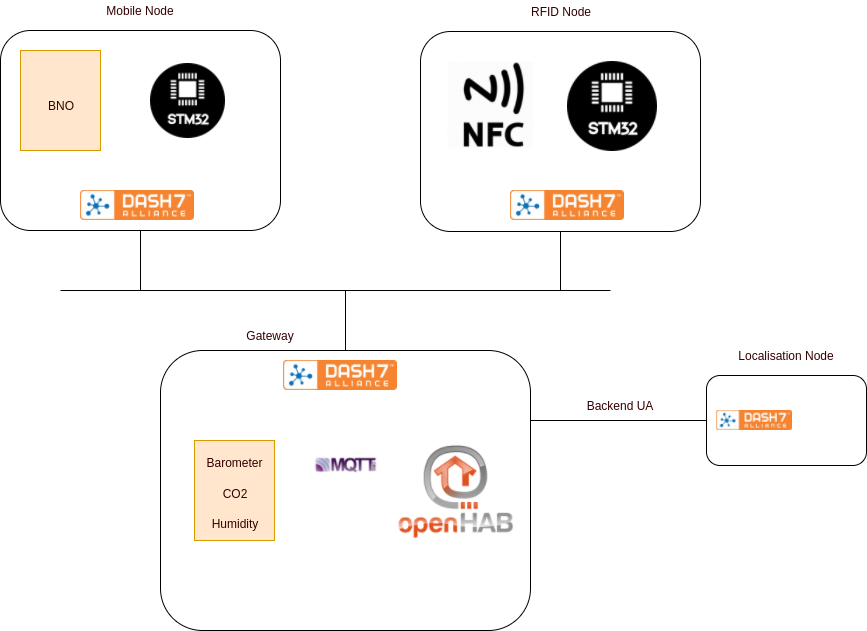
\includegraphics[width=\textwidth]{images/opbouw.png}
	\end{center}
\end{frame}

\note{Toelichten hoe het systeem is opgebouwd, zeggen dat mobiele node en RFID Node uitgelegd wordt doo kwinten, de localisatie door frederic en gateway openhab door seb en bernd.}


%%%%%%%%%%%%%%%%%%%%%%%%%%%%%%%%%%%%%%%%%%%%%%%%%%%%%%%%%%%%%%%%%%%%%%%%%%%%%%%%%%%%%%%%%%
\section{External Nodes}
%%%%%%%%%%%%%%%%%%%%%%%%%%%%%%%%%%%%%%%%%%%%%%%%%%%%%%%%%%%%%%%%%%%%%%%%%%%%%%%%%%%%%%%%%%

\subsection{NFC Node}

\begin{frame}[fragile]
\frametitle{NFC Node - Eagle} 
\begin{figure}
  \centering
  \subfloat{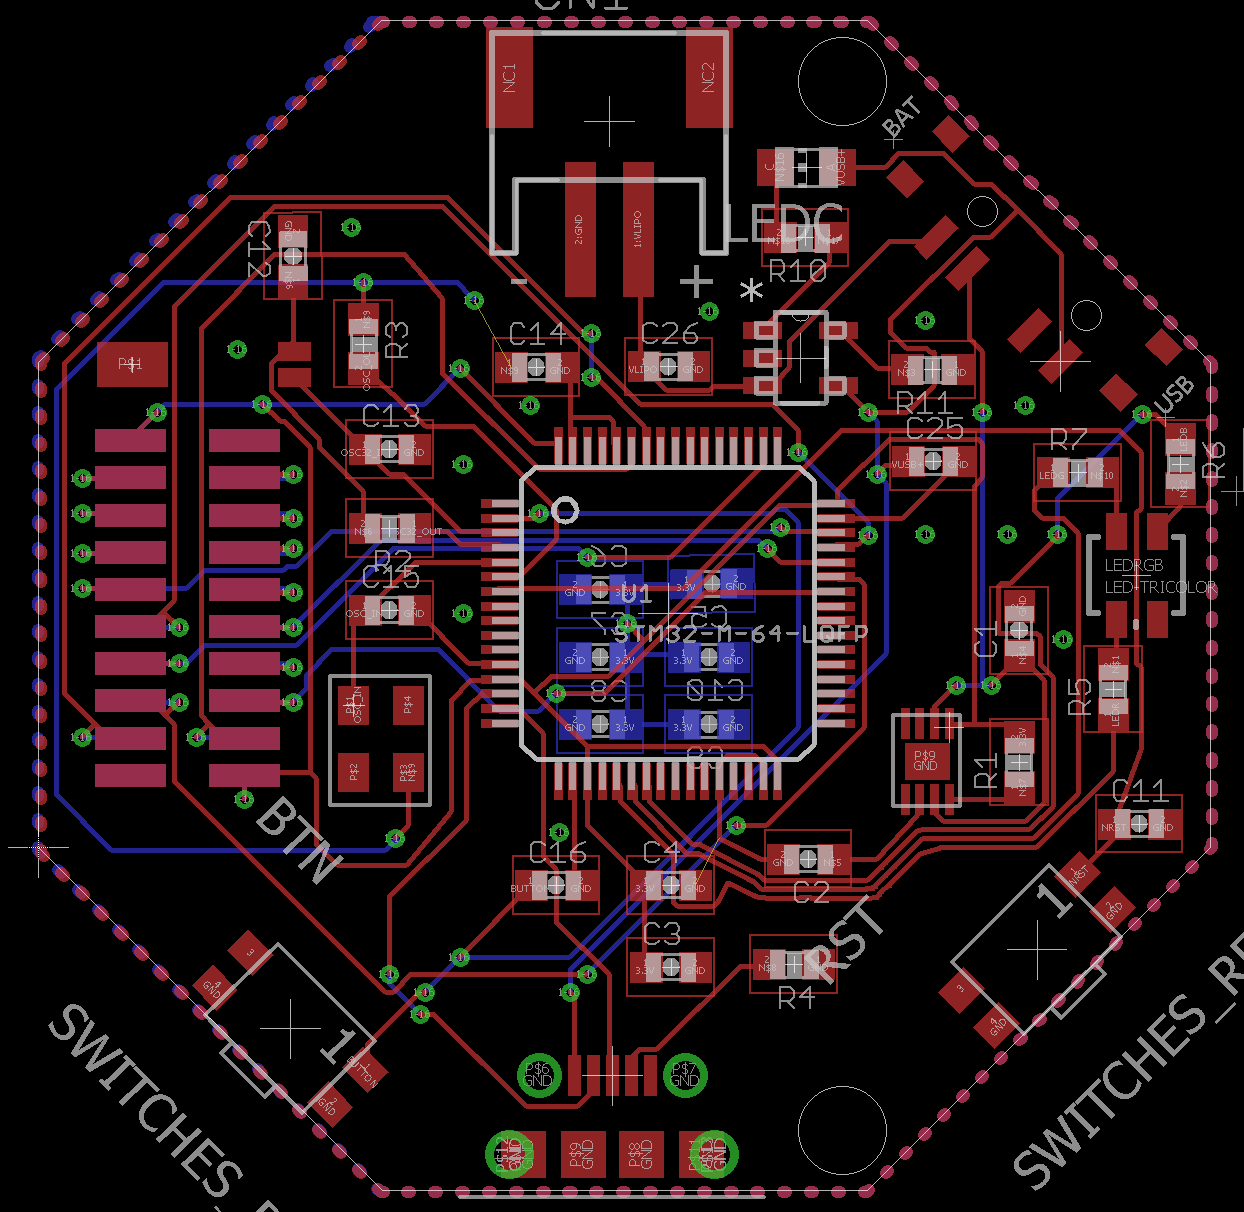
\includegraphics[width=.4\textwidth]{images/eagle1.png}}\qquad
  \subfloat{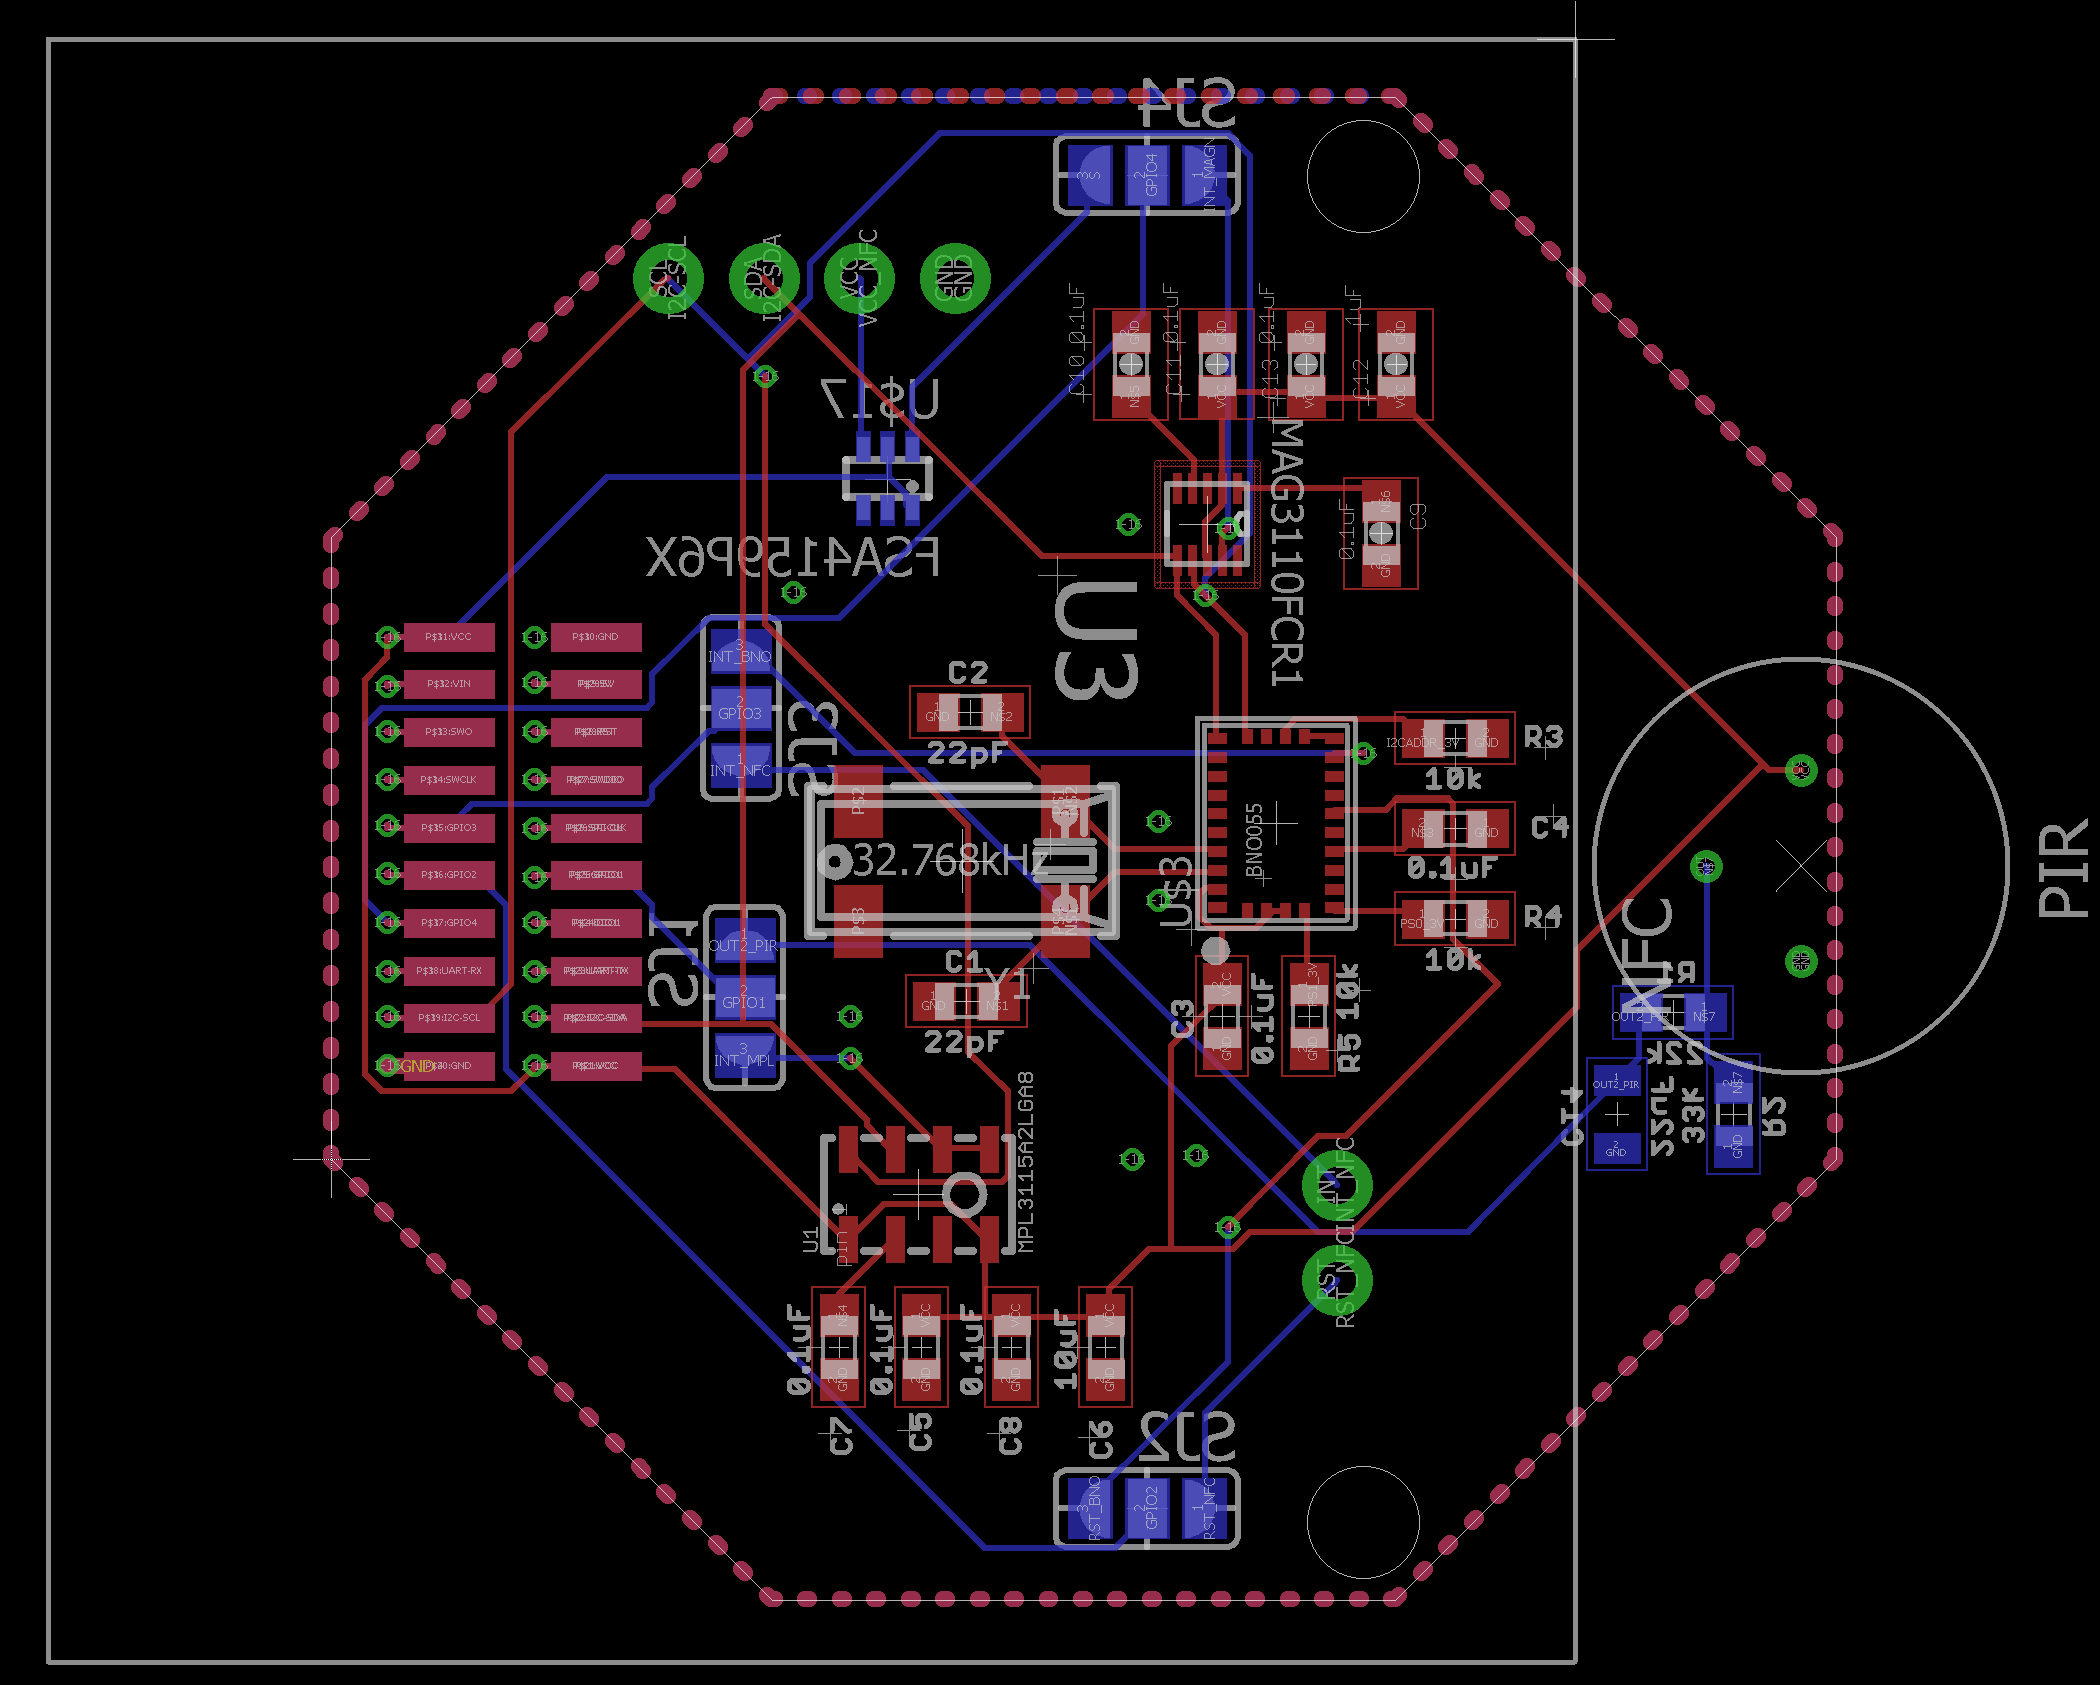
\includegraphics[width=.4\textwidth]{images/eagle2.png}}
\end{figure}
\end{frame}

\begin{frame}[fragile]
\frametitle{NFC Node - Hardware} 
\begin{figure}
  \centering
  \subfloat{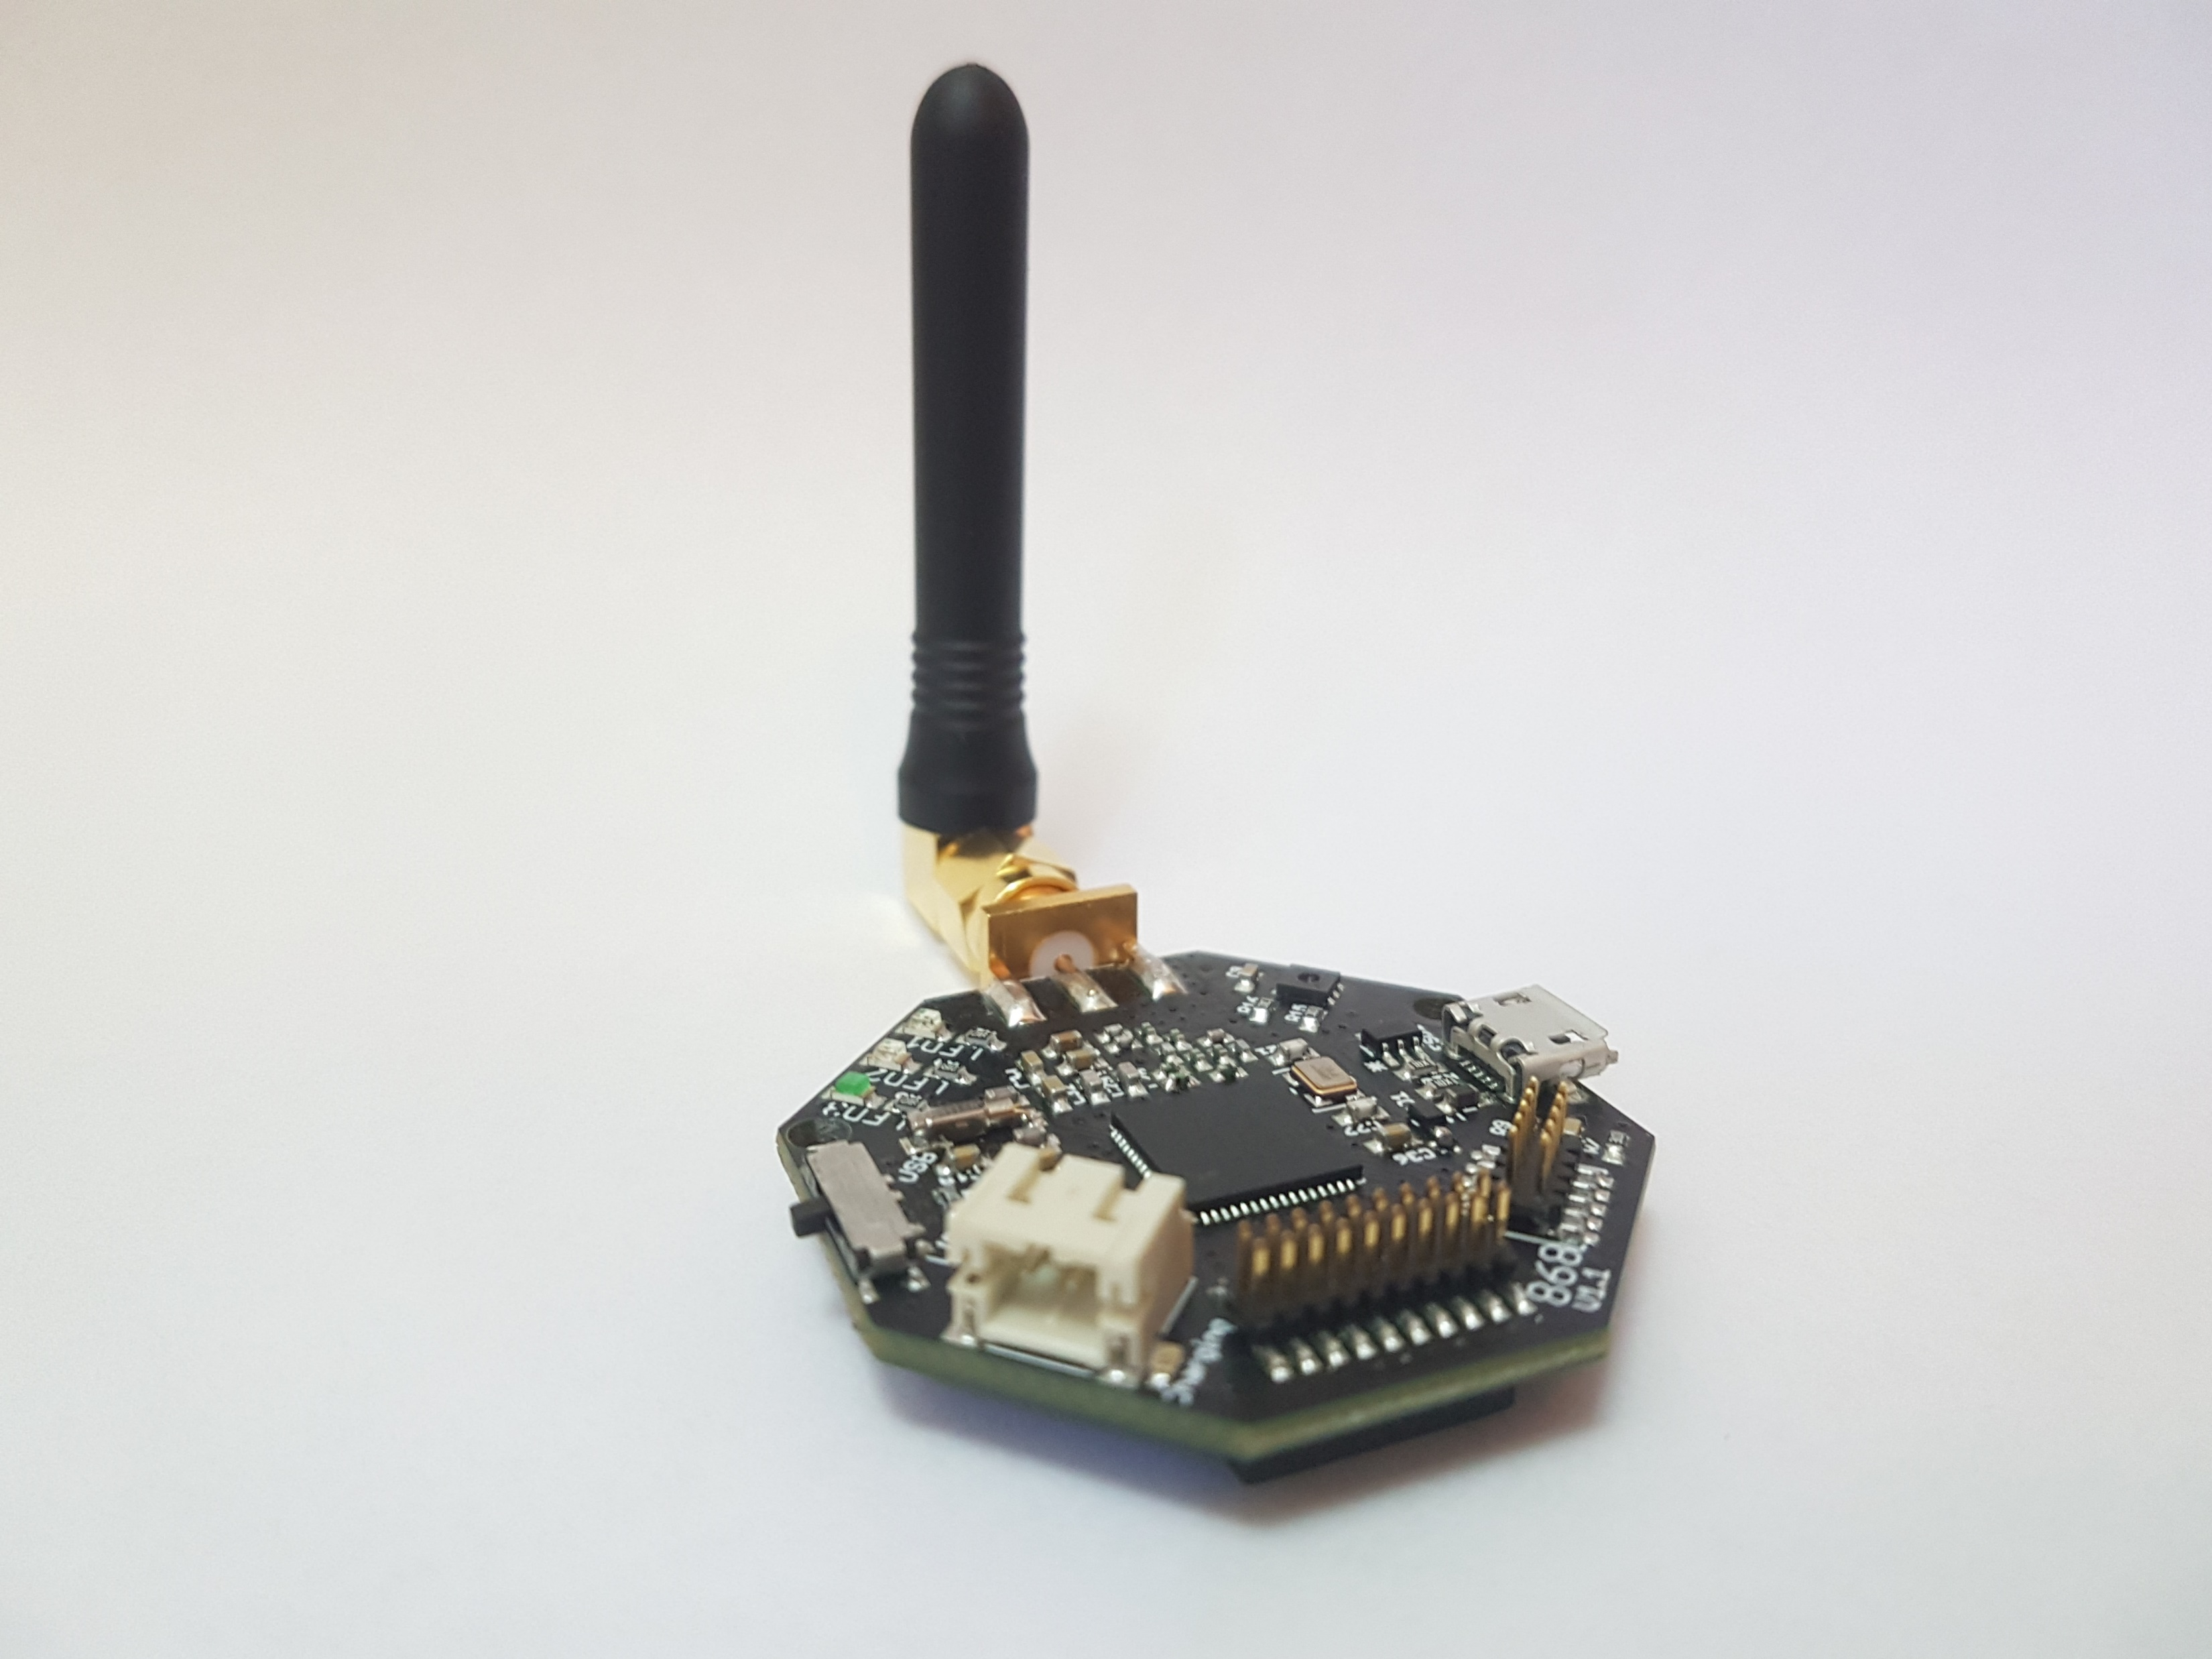
\includegraphics[width=.4\textwidth]{images/NFC1.jpg}}\qquad
  \subfloat{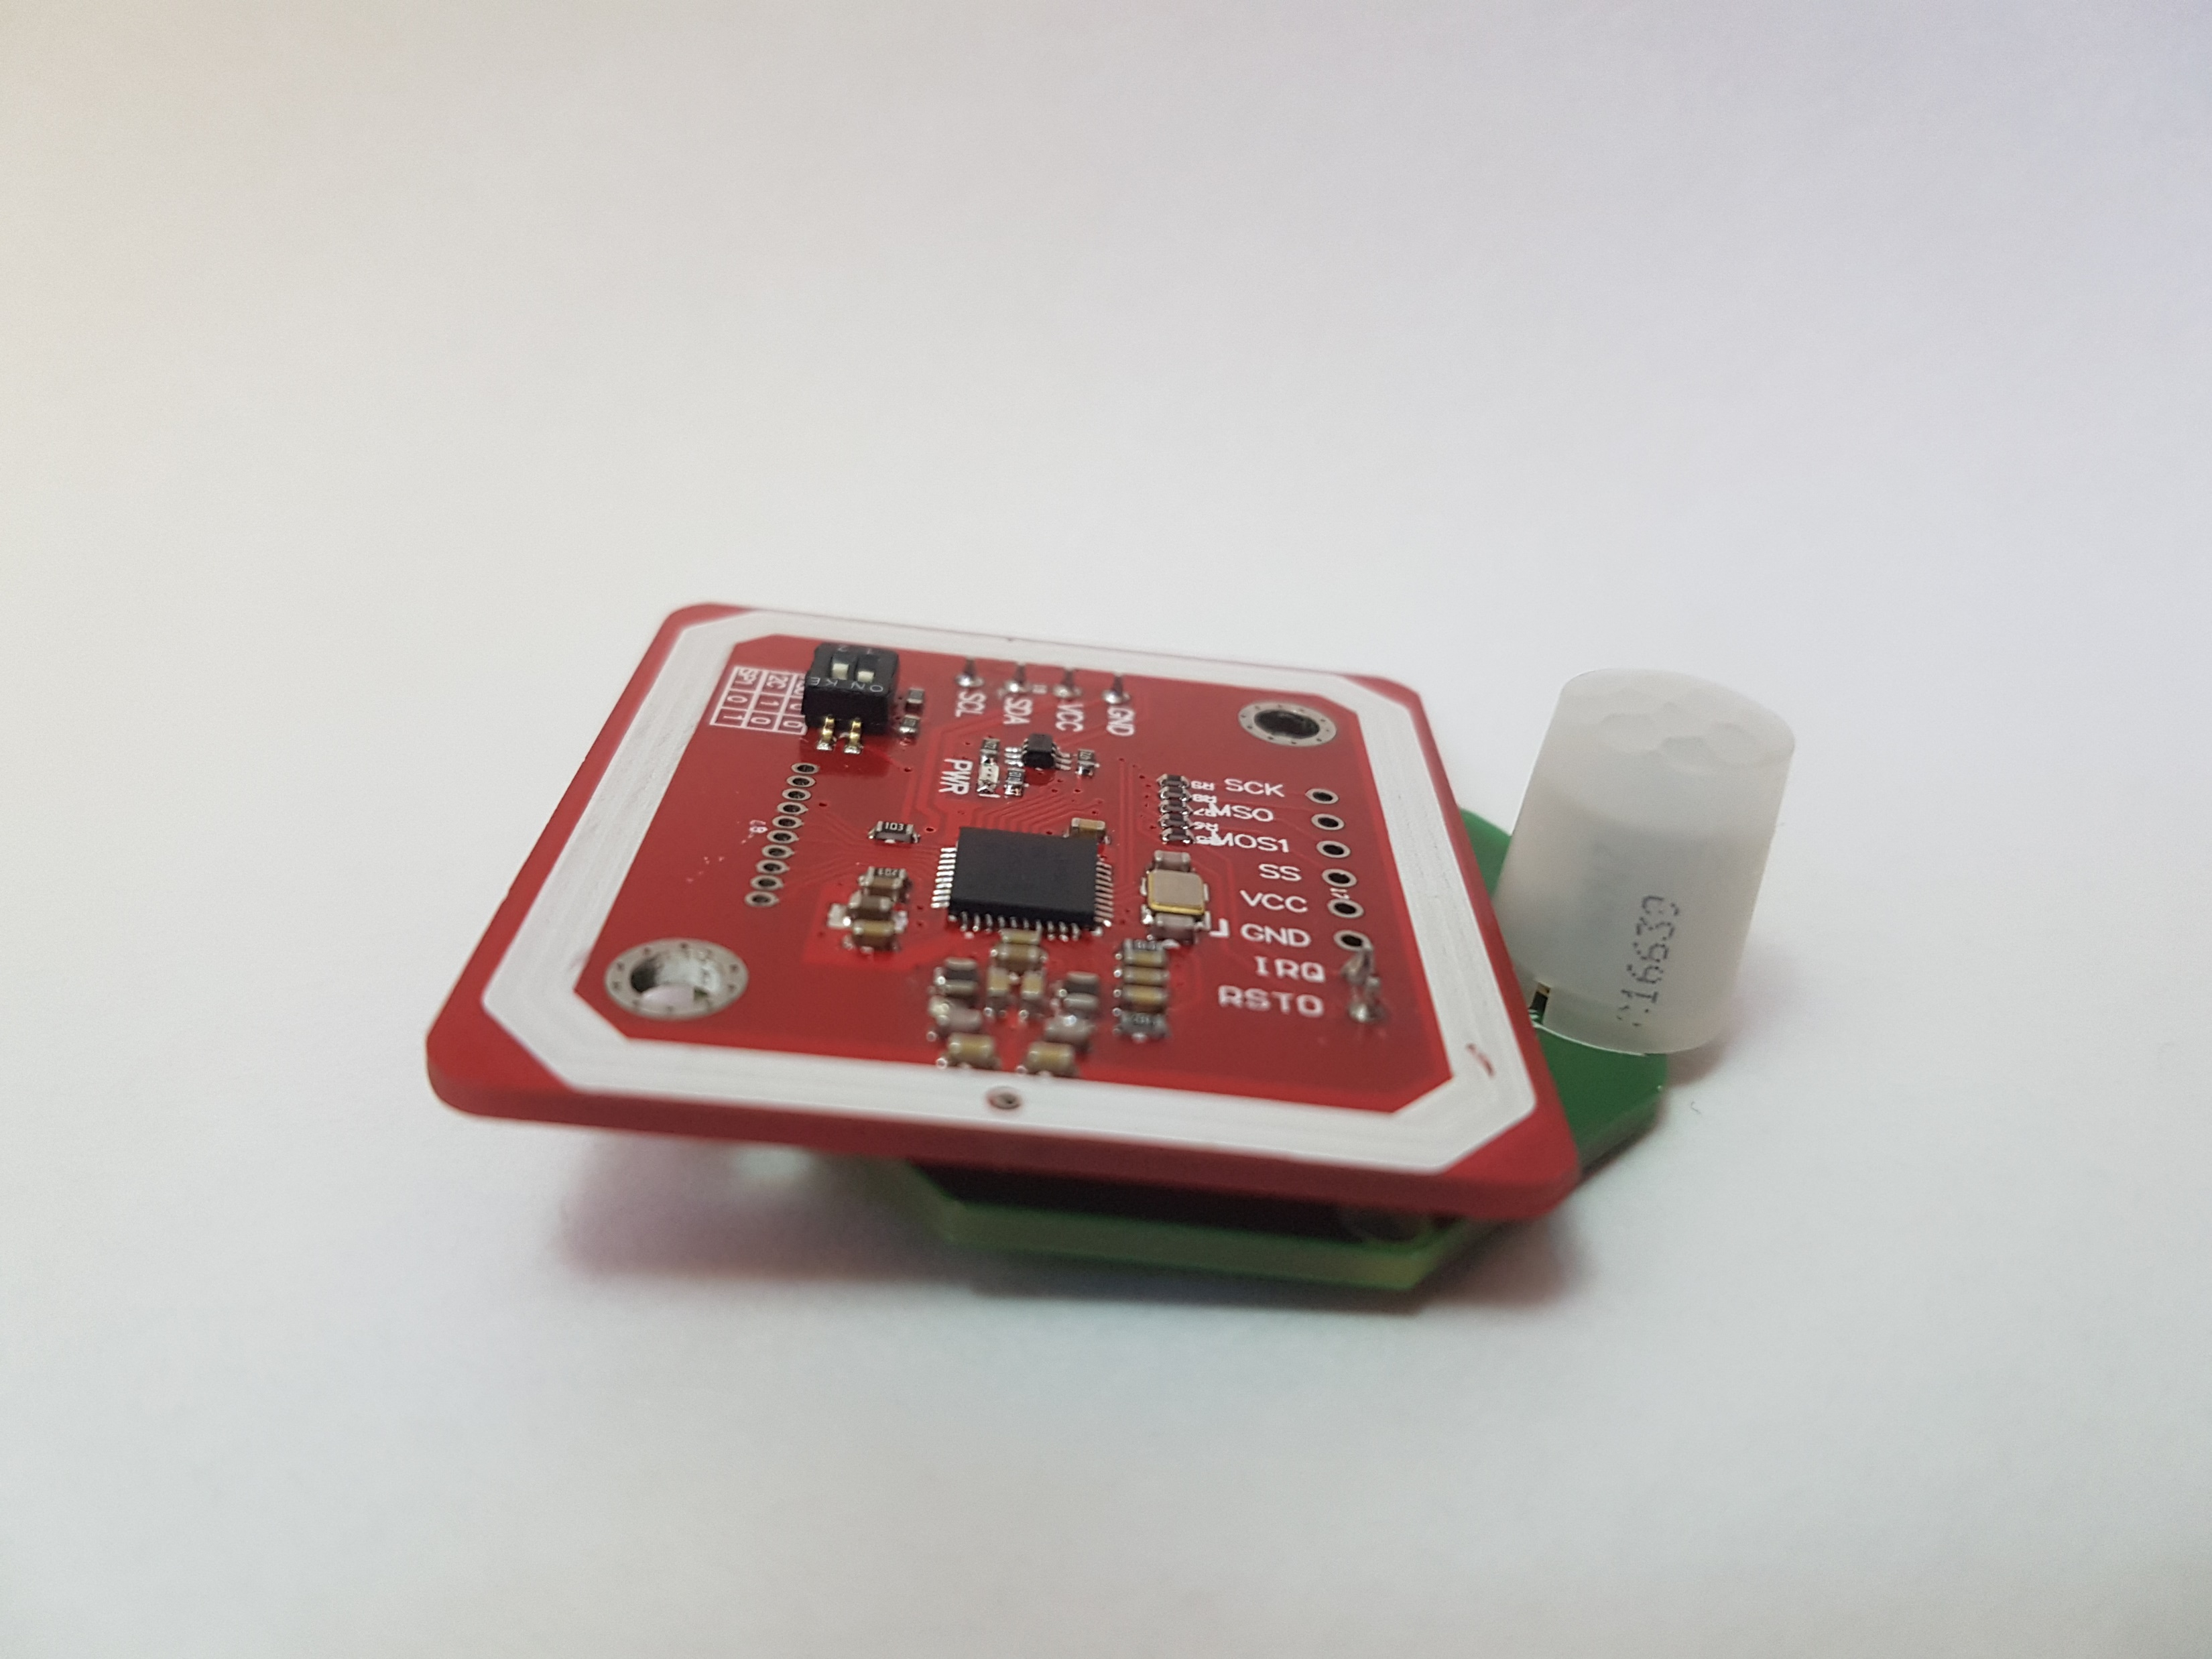
\includegraphics[width=.4\textwidth]{images/NFC2.jpg}}
\end{figure}
\begin{figure}
  \centering
  \subfloat{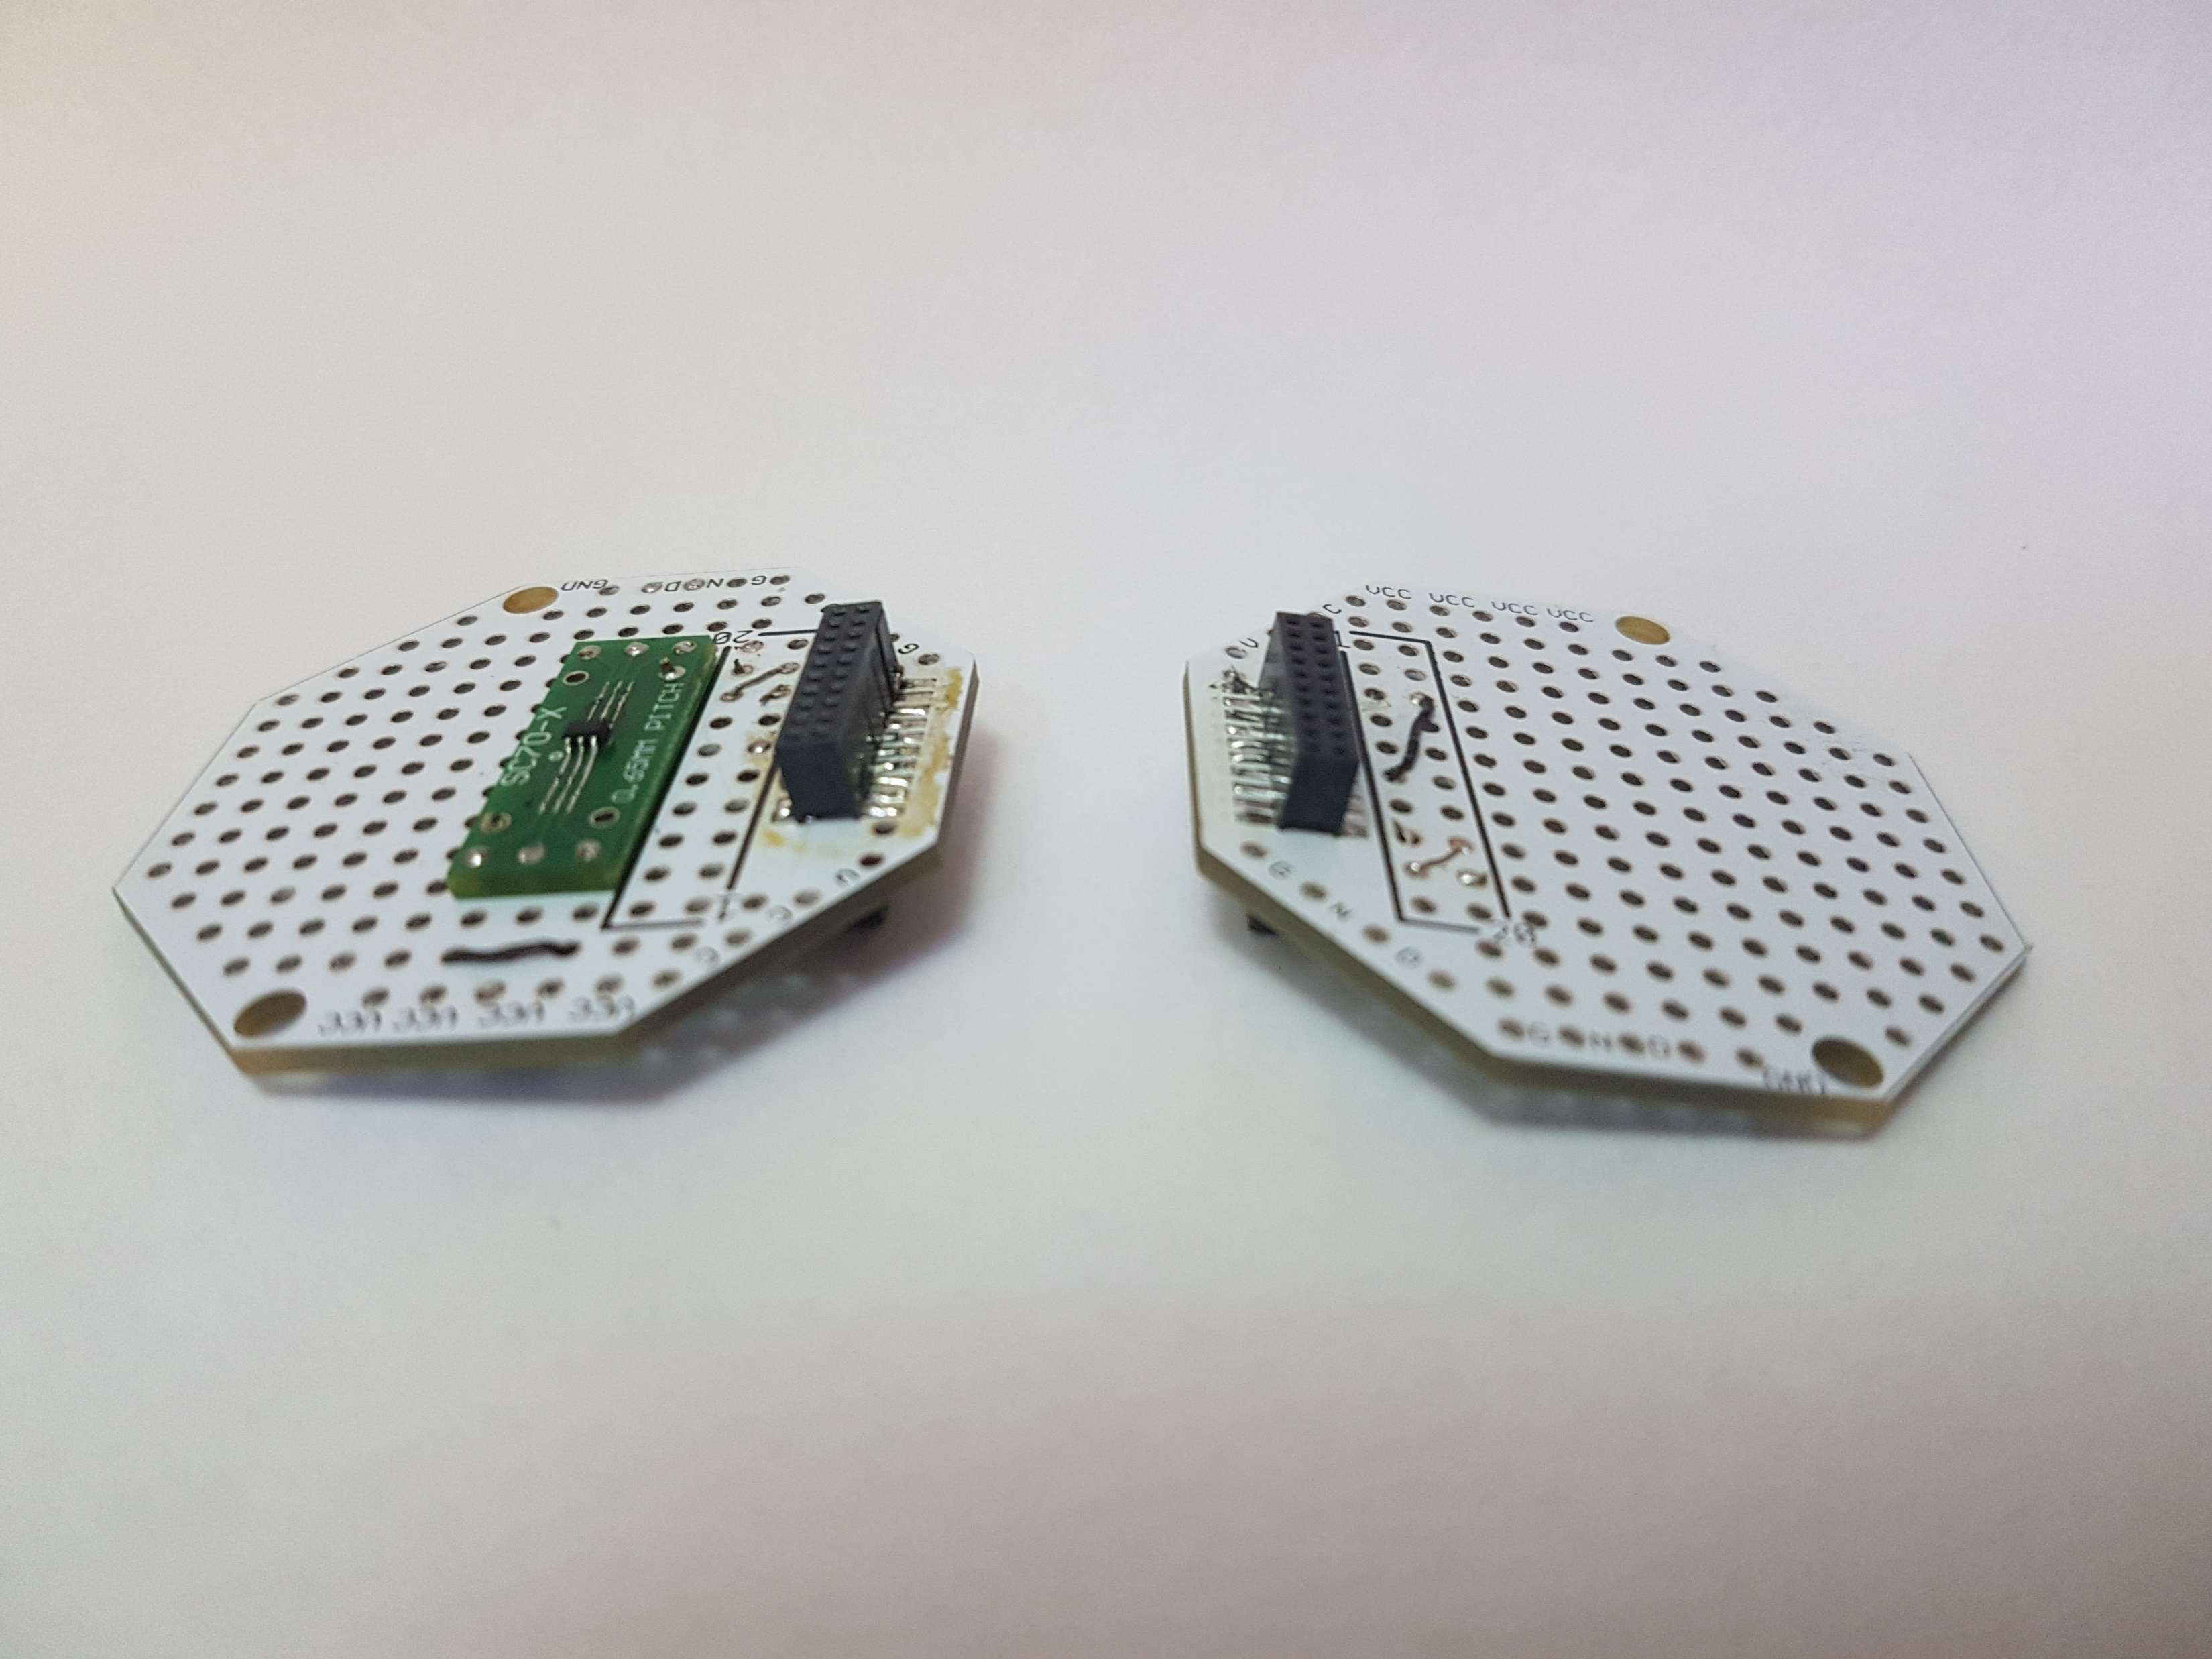
\includegraphics[width=.4\textwidth]{images/NFC3.jpg}}\qquad
  \subfloat{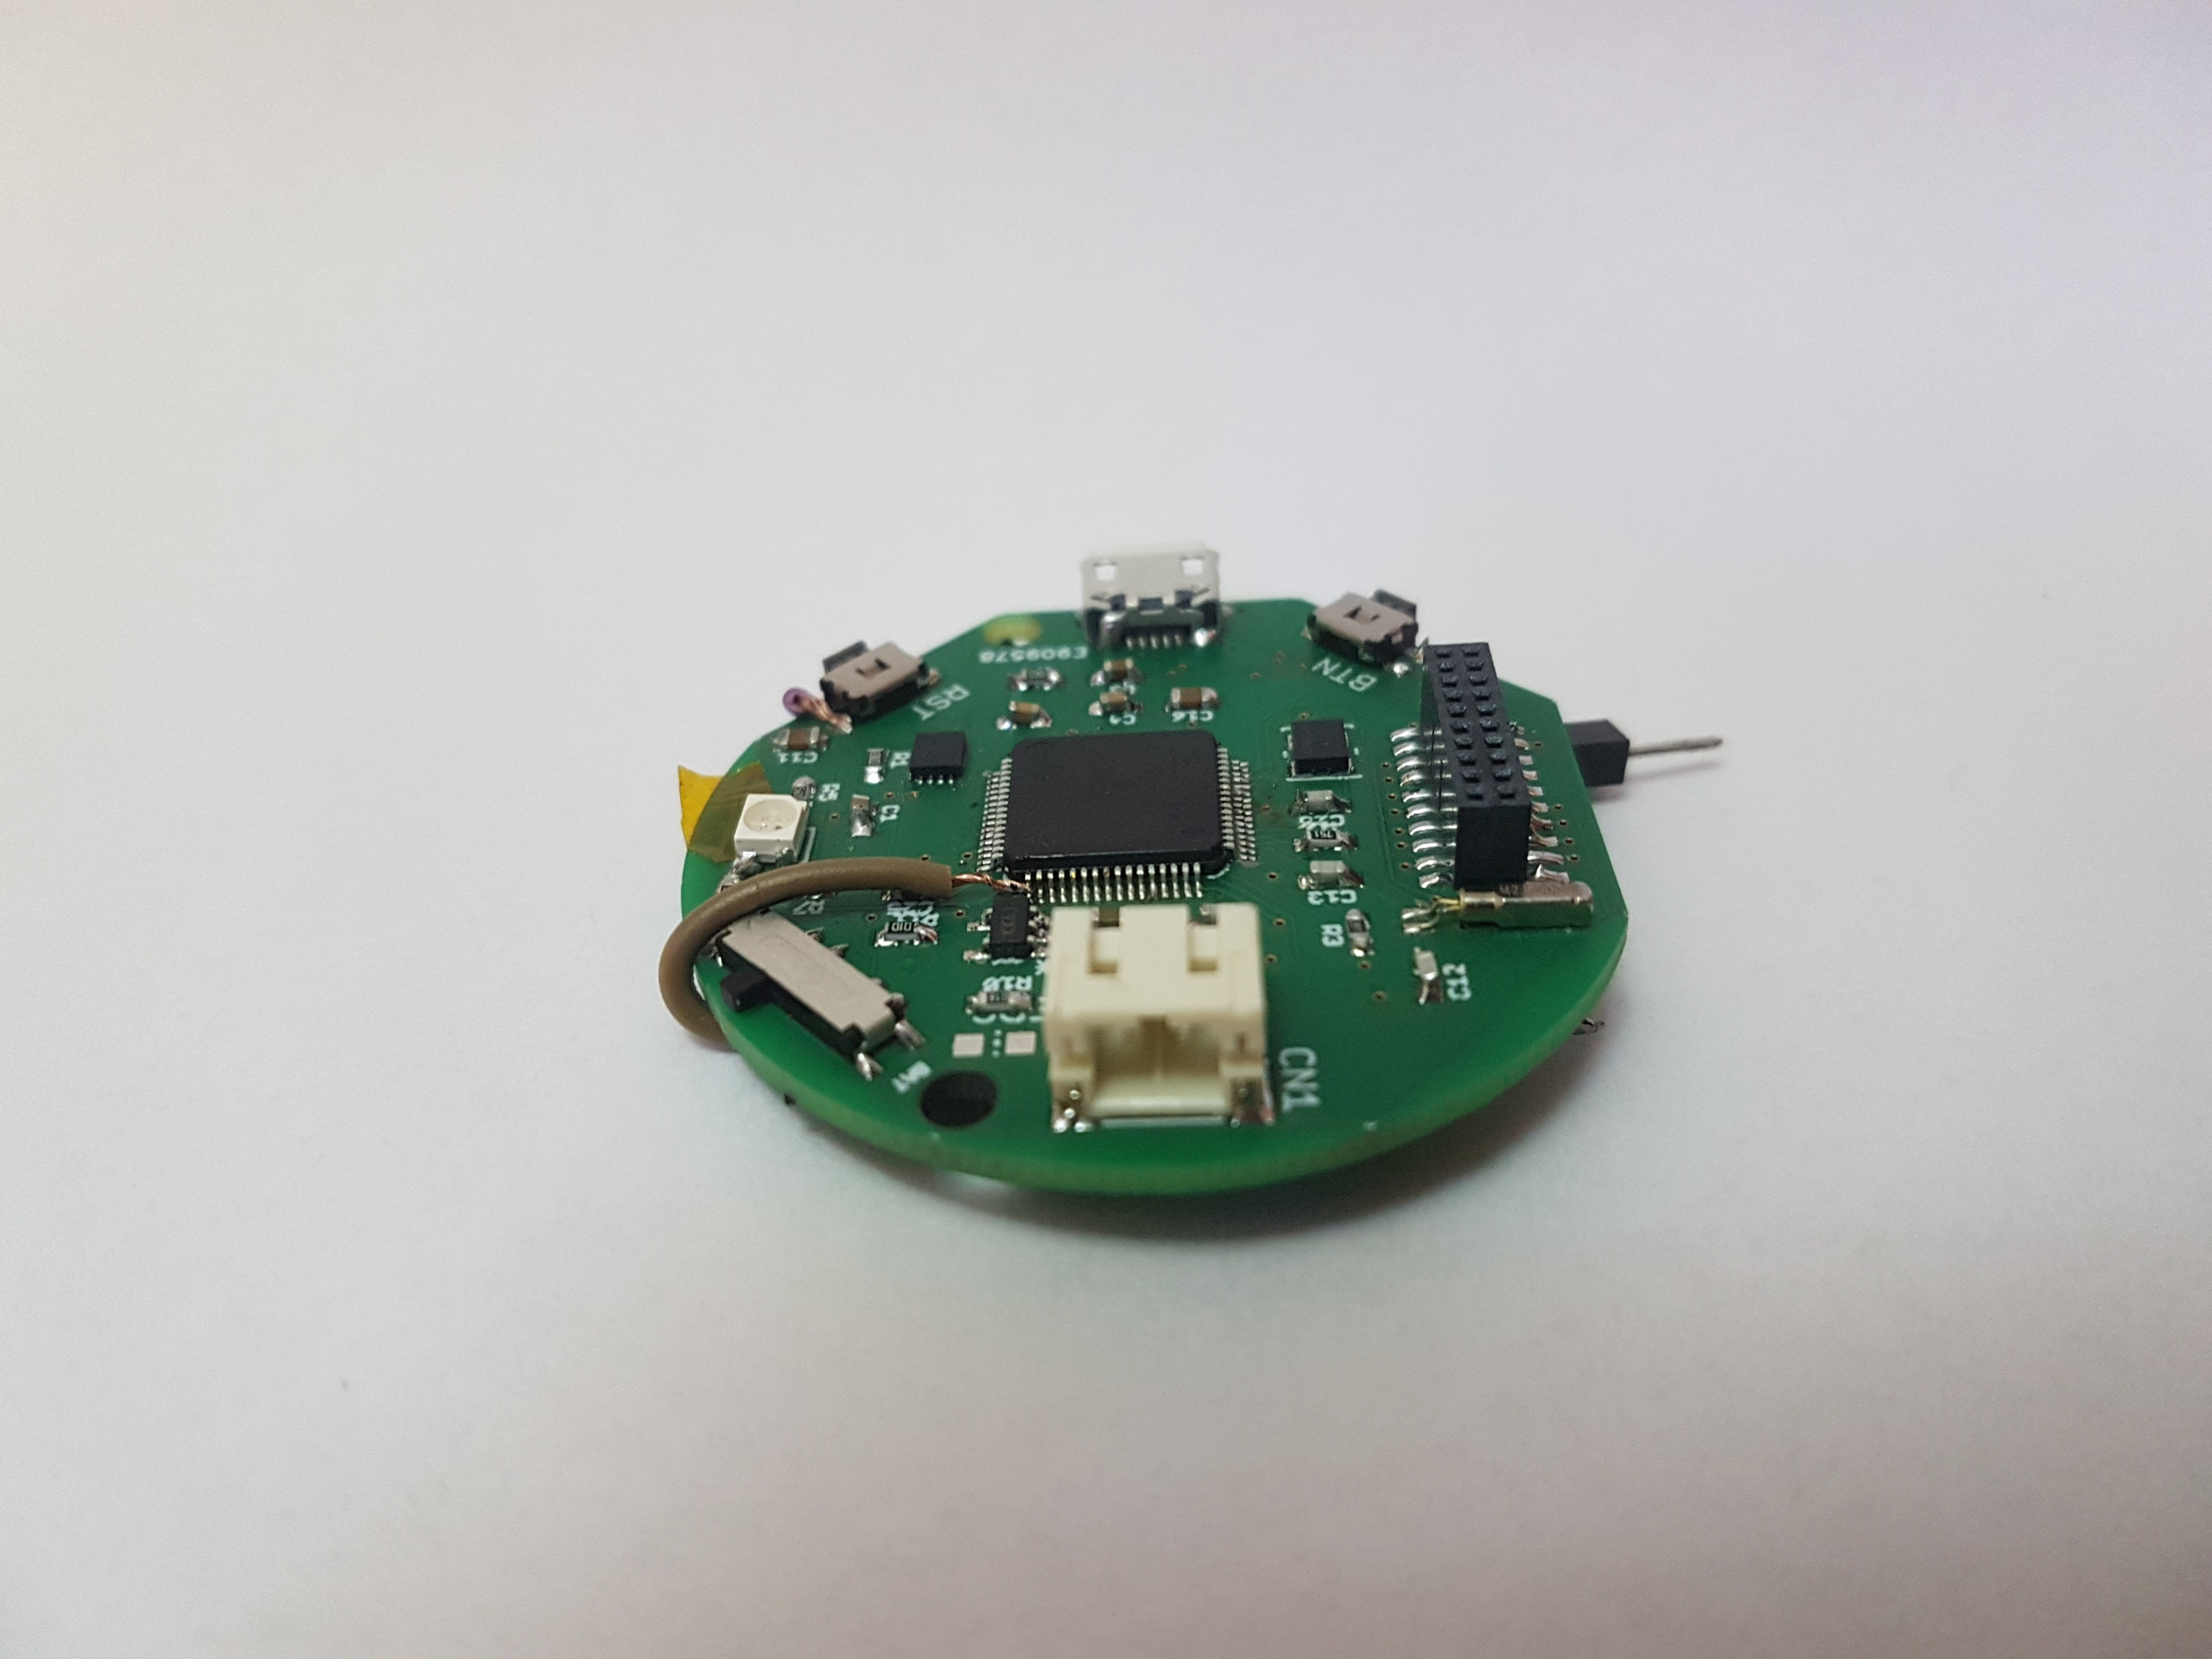
\includegraphics[width=.4\textwidth]{images/NFC4.jpg}}
\end{figure}
\end{frame}

\begin{frame}[fragile]
\frametitle{NFC Node - Combinatie} 
\begin{figure}
  \centering
  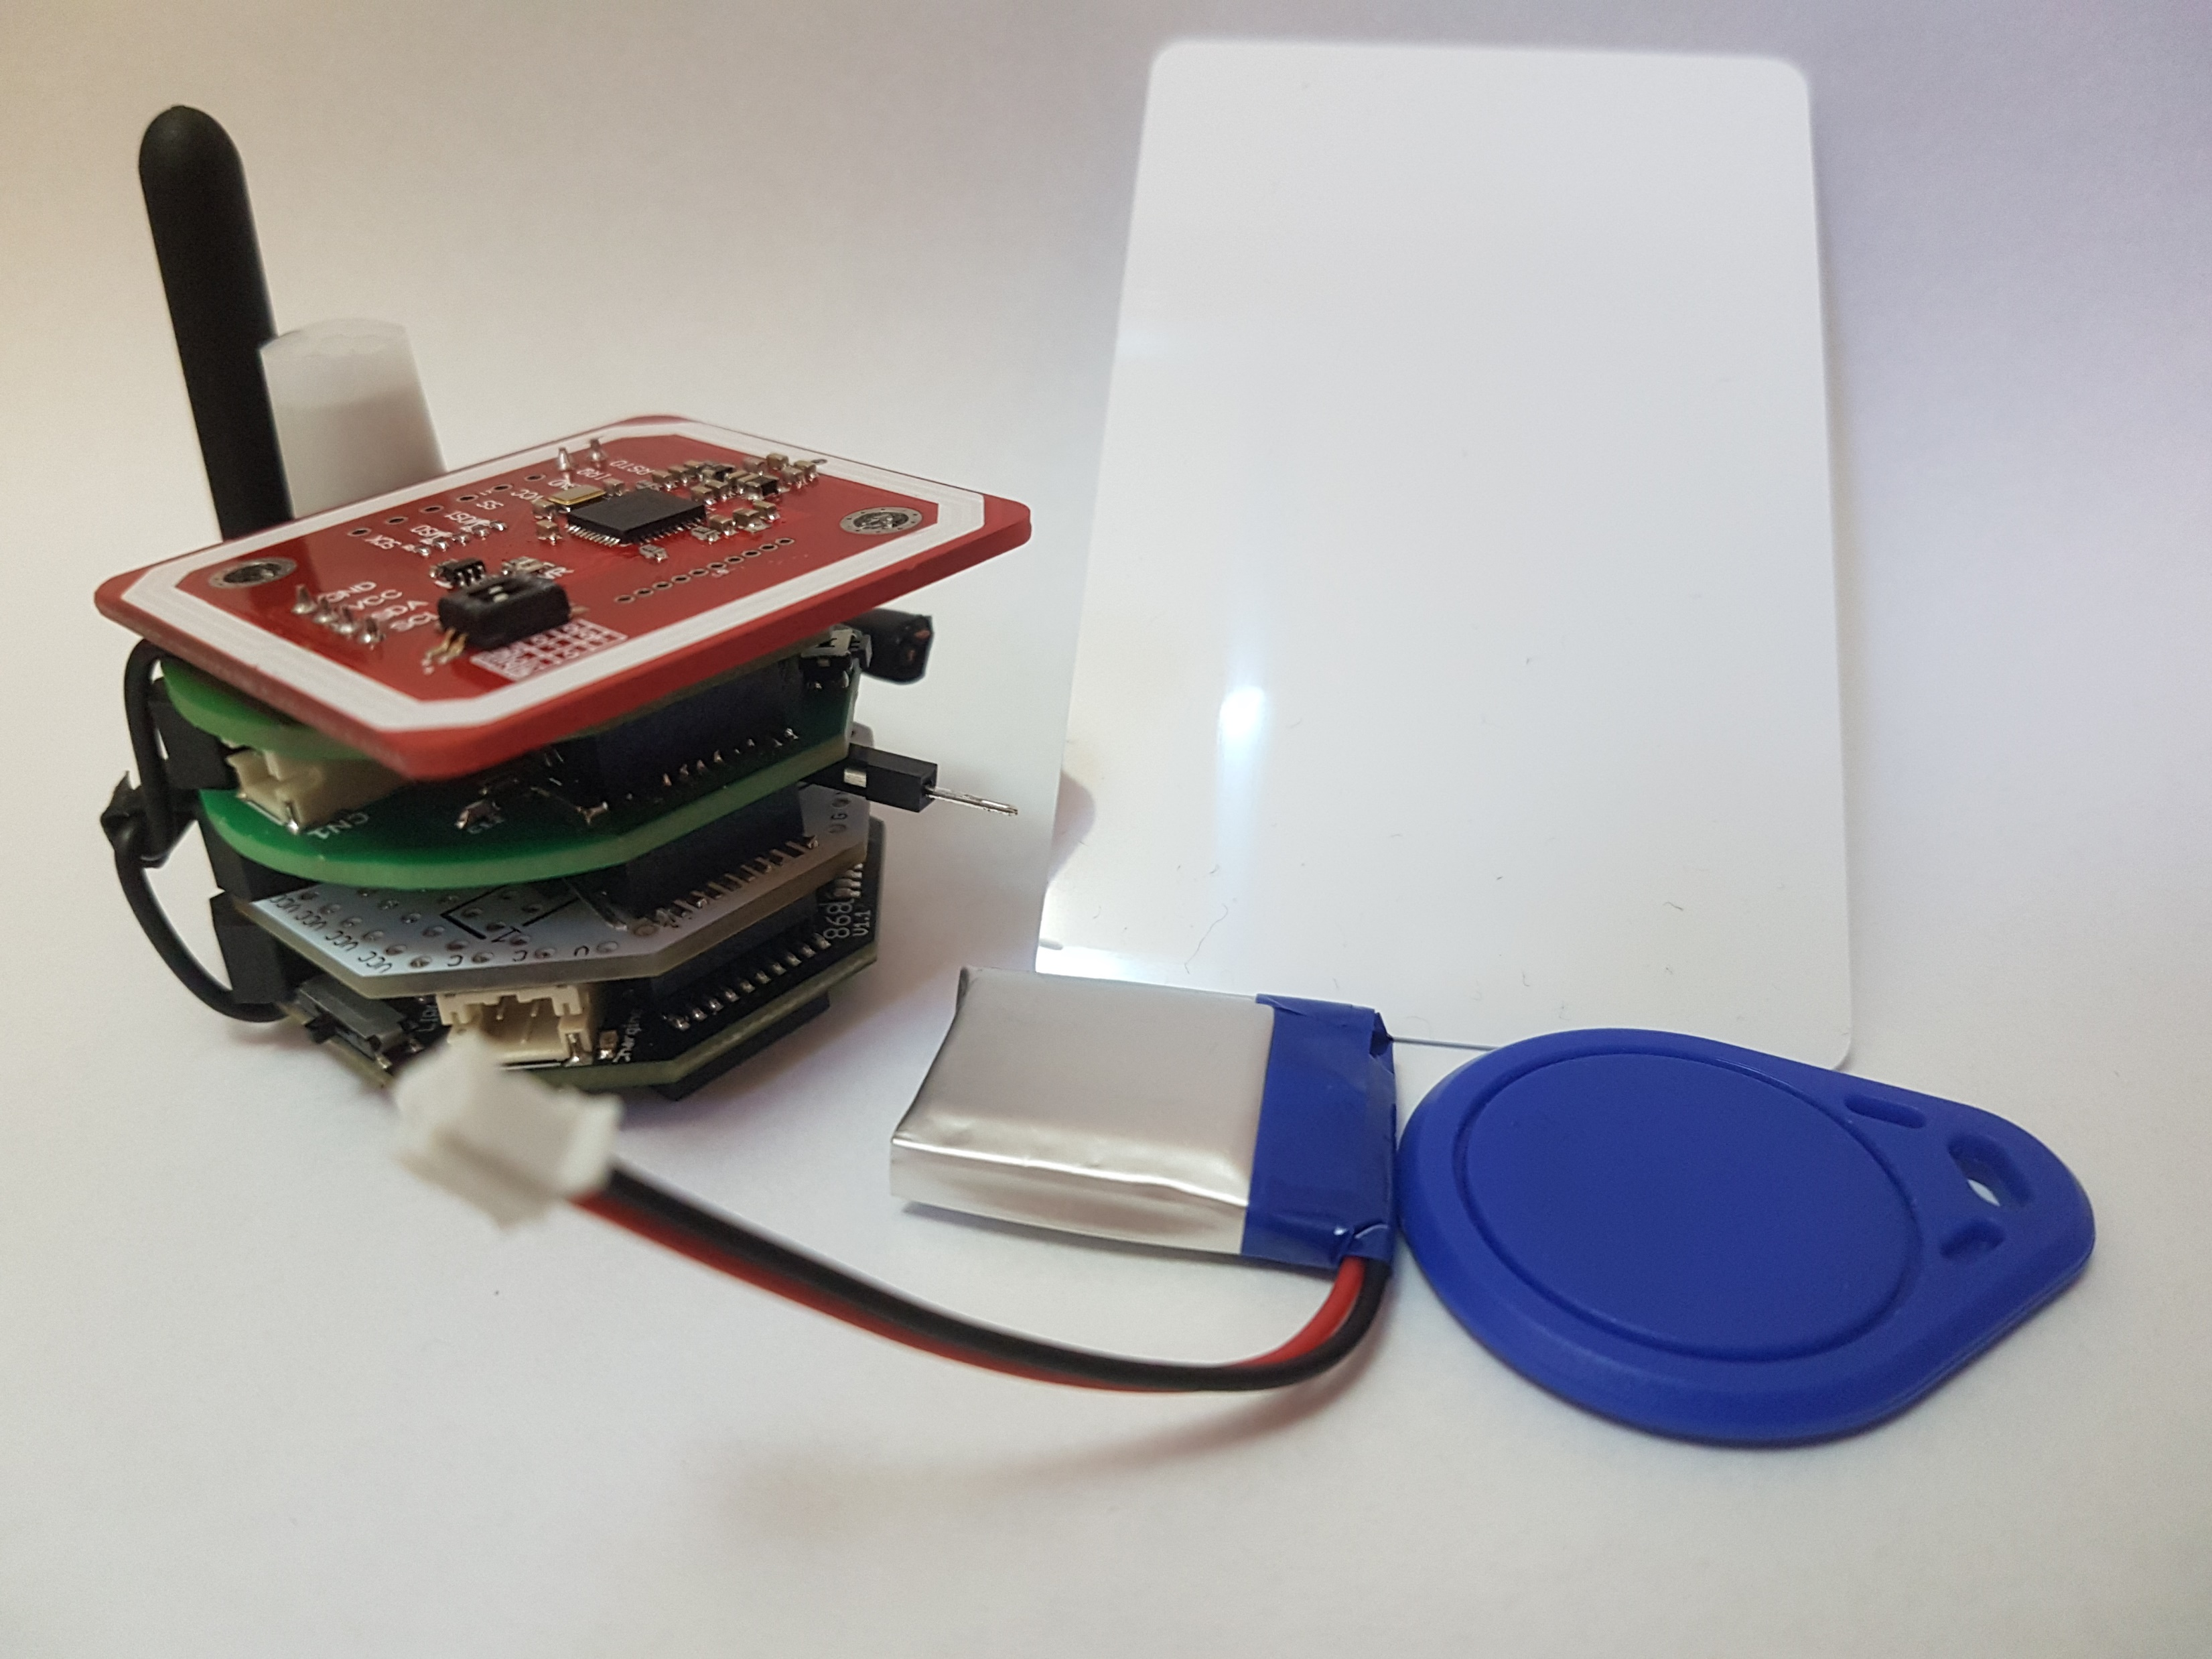
\includegraphics[width=\textwidth]{images/NFC5.jpg}
\end{figure}
\end{frame}

\begin{frame}[fragile]
\frametitle{NFC Node - Software} 
\begin{figure}
  \centering
  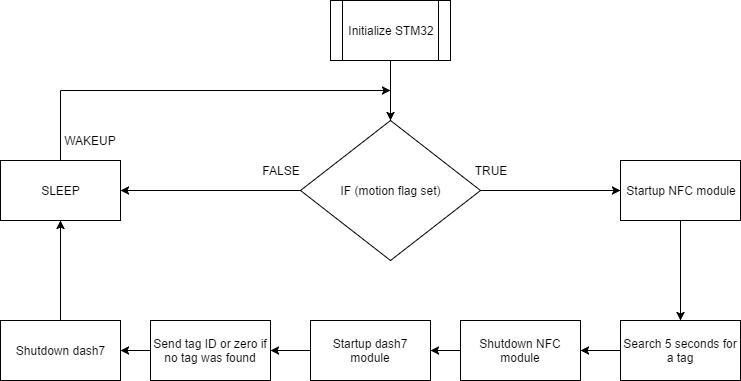
\includegraphics[width=\textwidth]{images/NFC6.png}
\end{figure}
\end{frame}

\begin{frame}[fragile]
\frametitle{NFC Node - Power Management} 
\begin{figure}
  \centering
  \subfloat{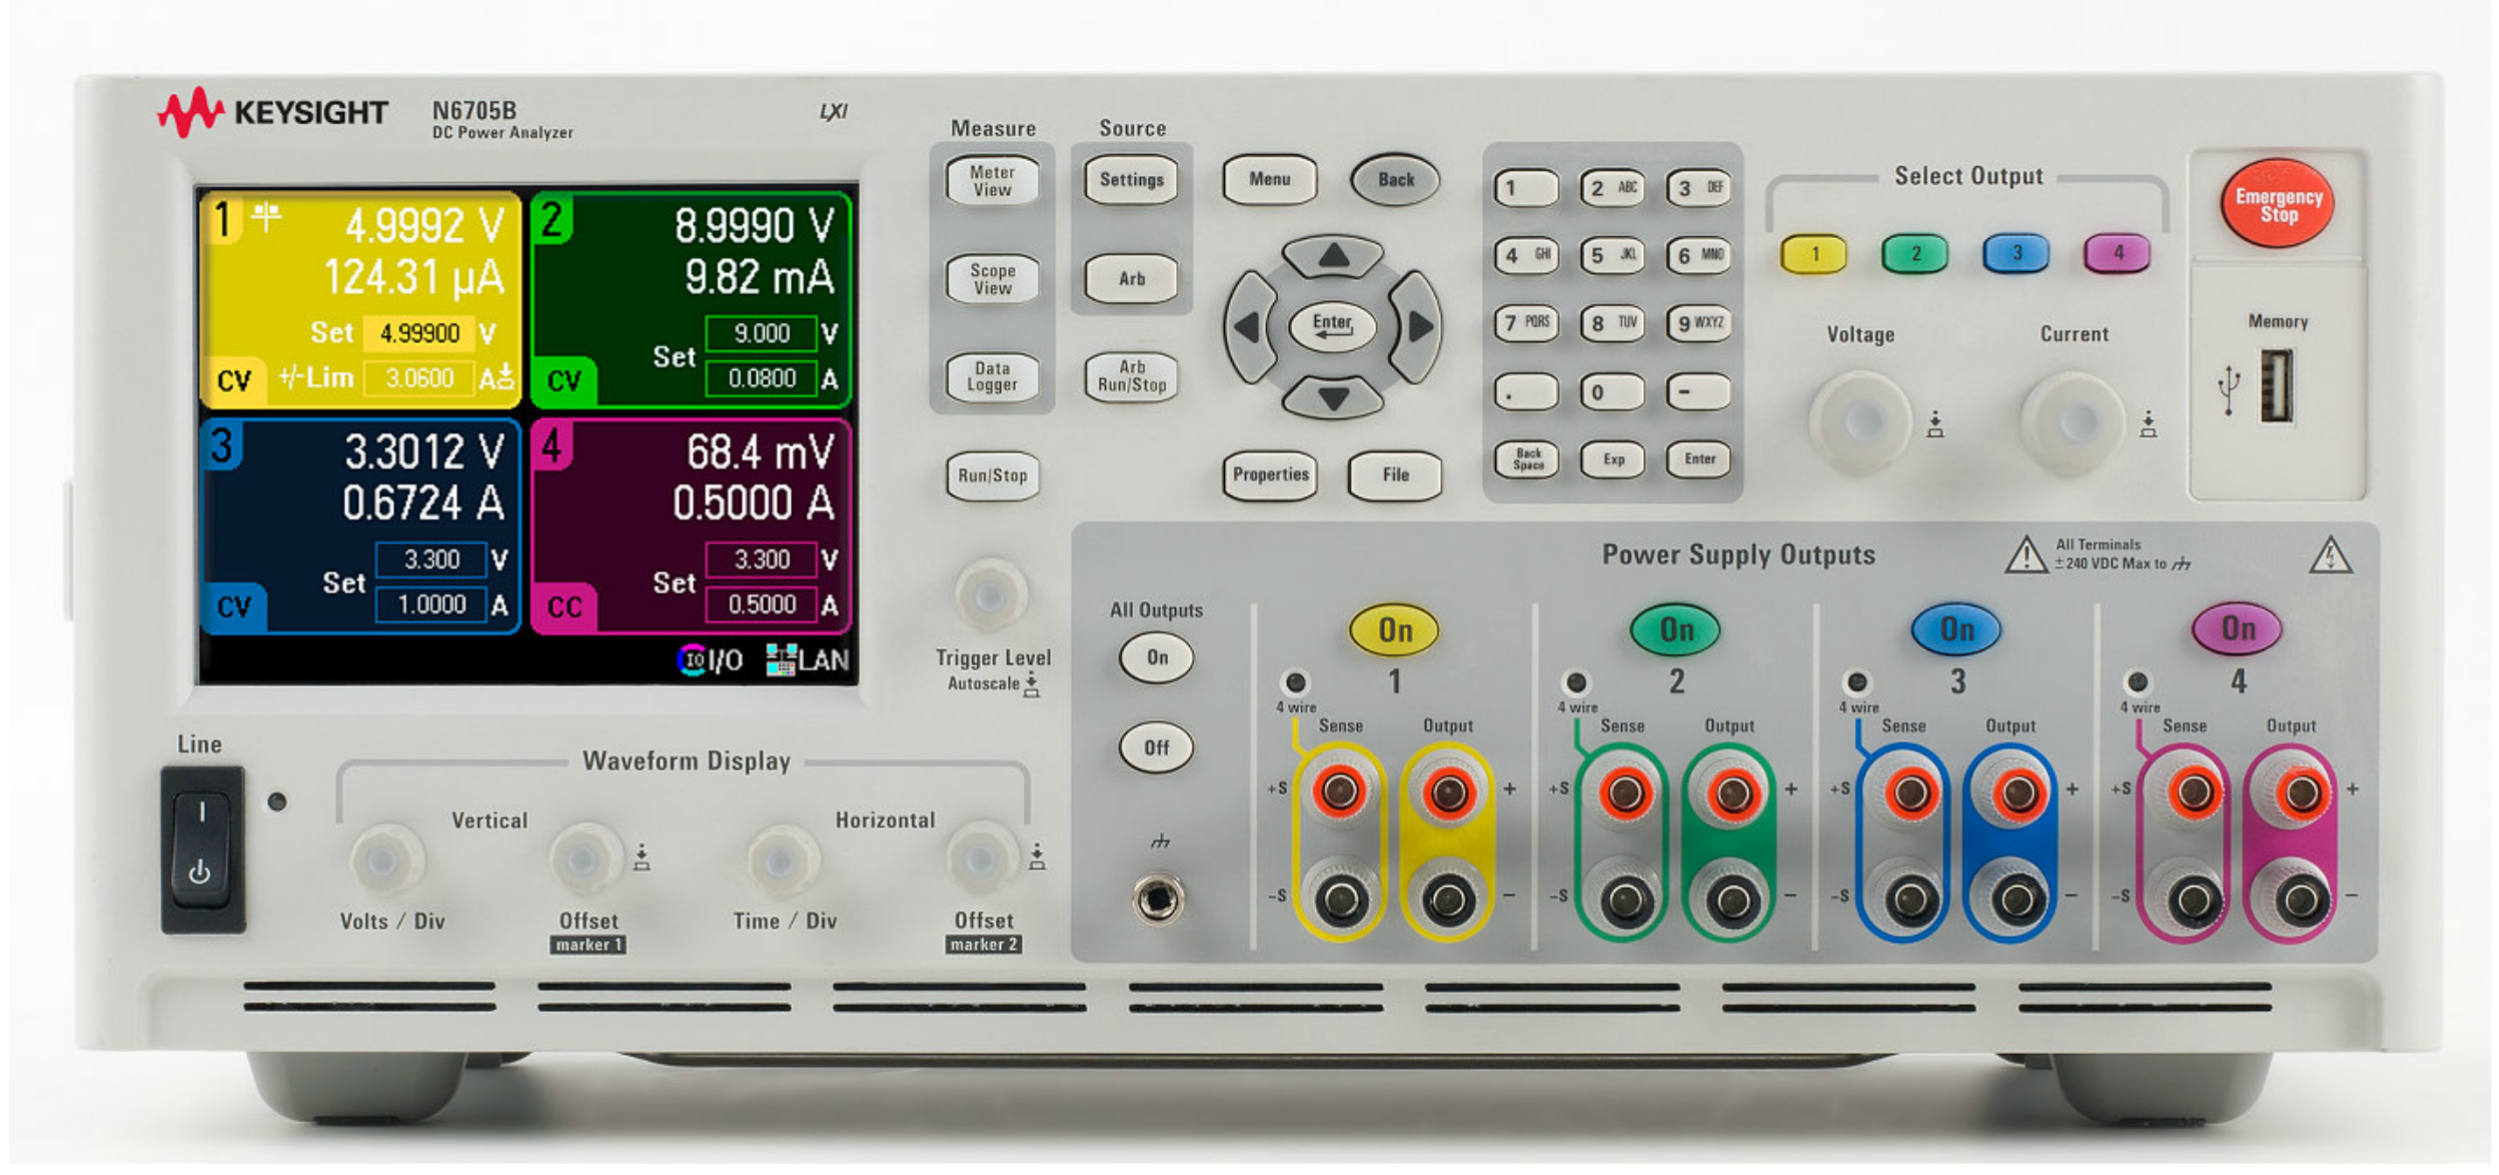
\includegraphics[width=.5\textwidth]{images/NFC7.png}}\qquad
  \subfloat{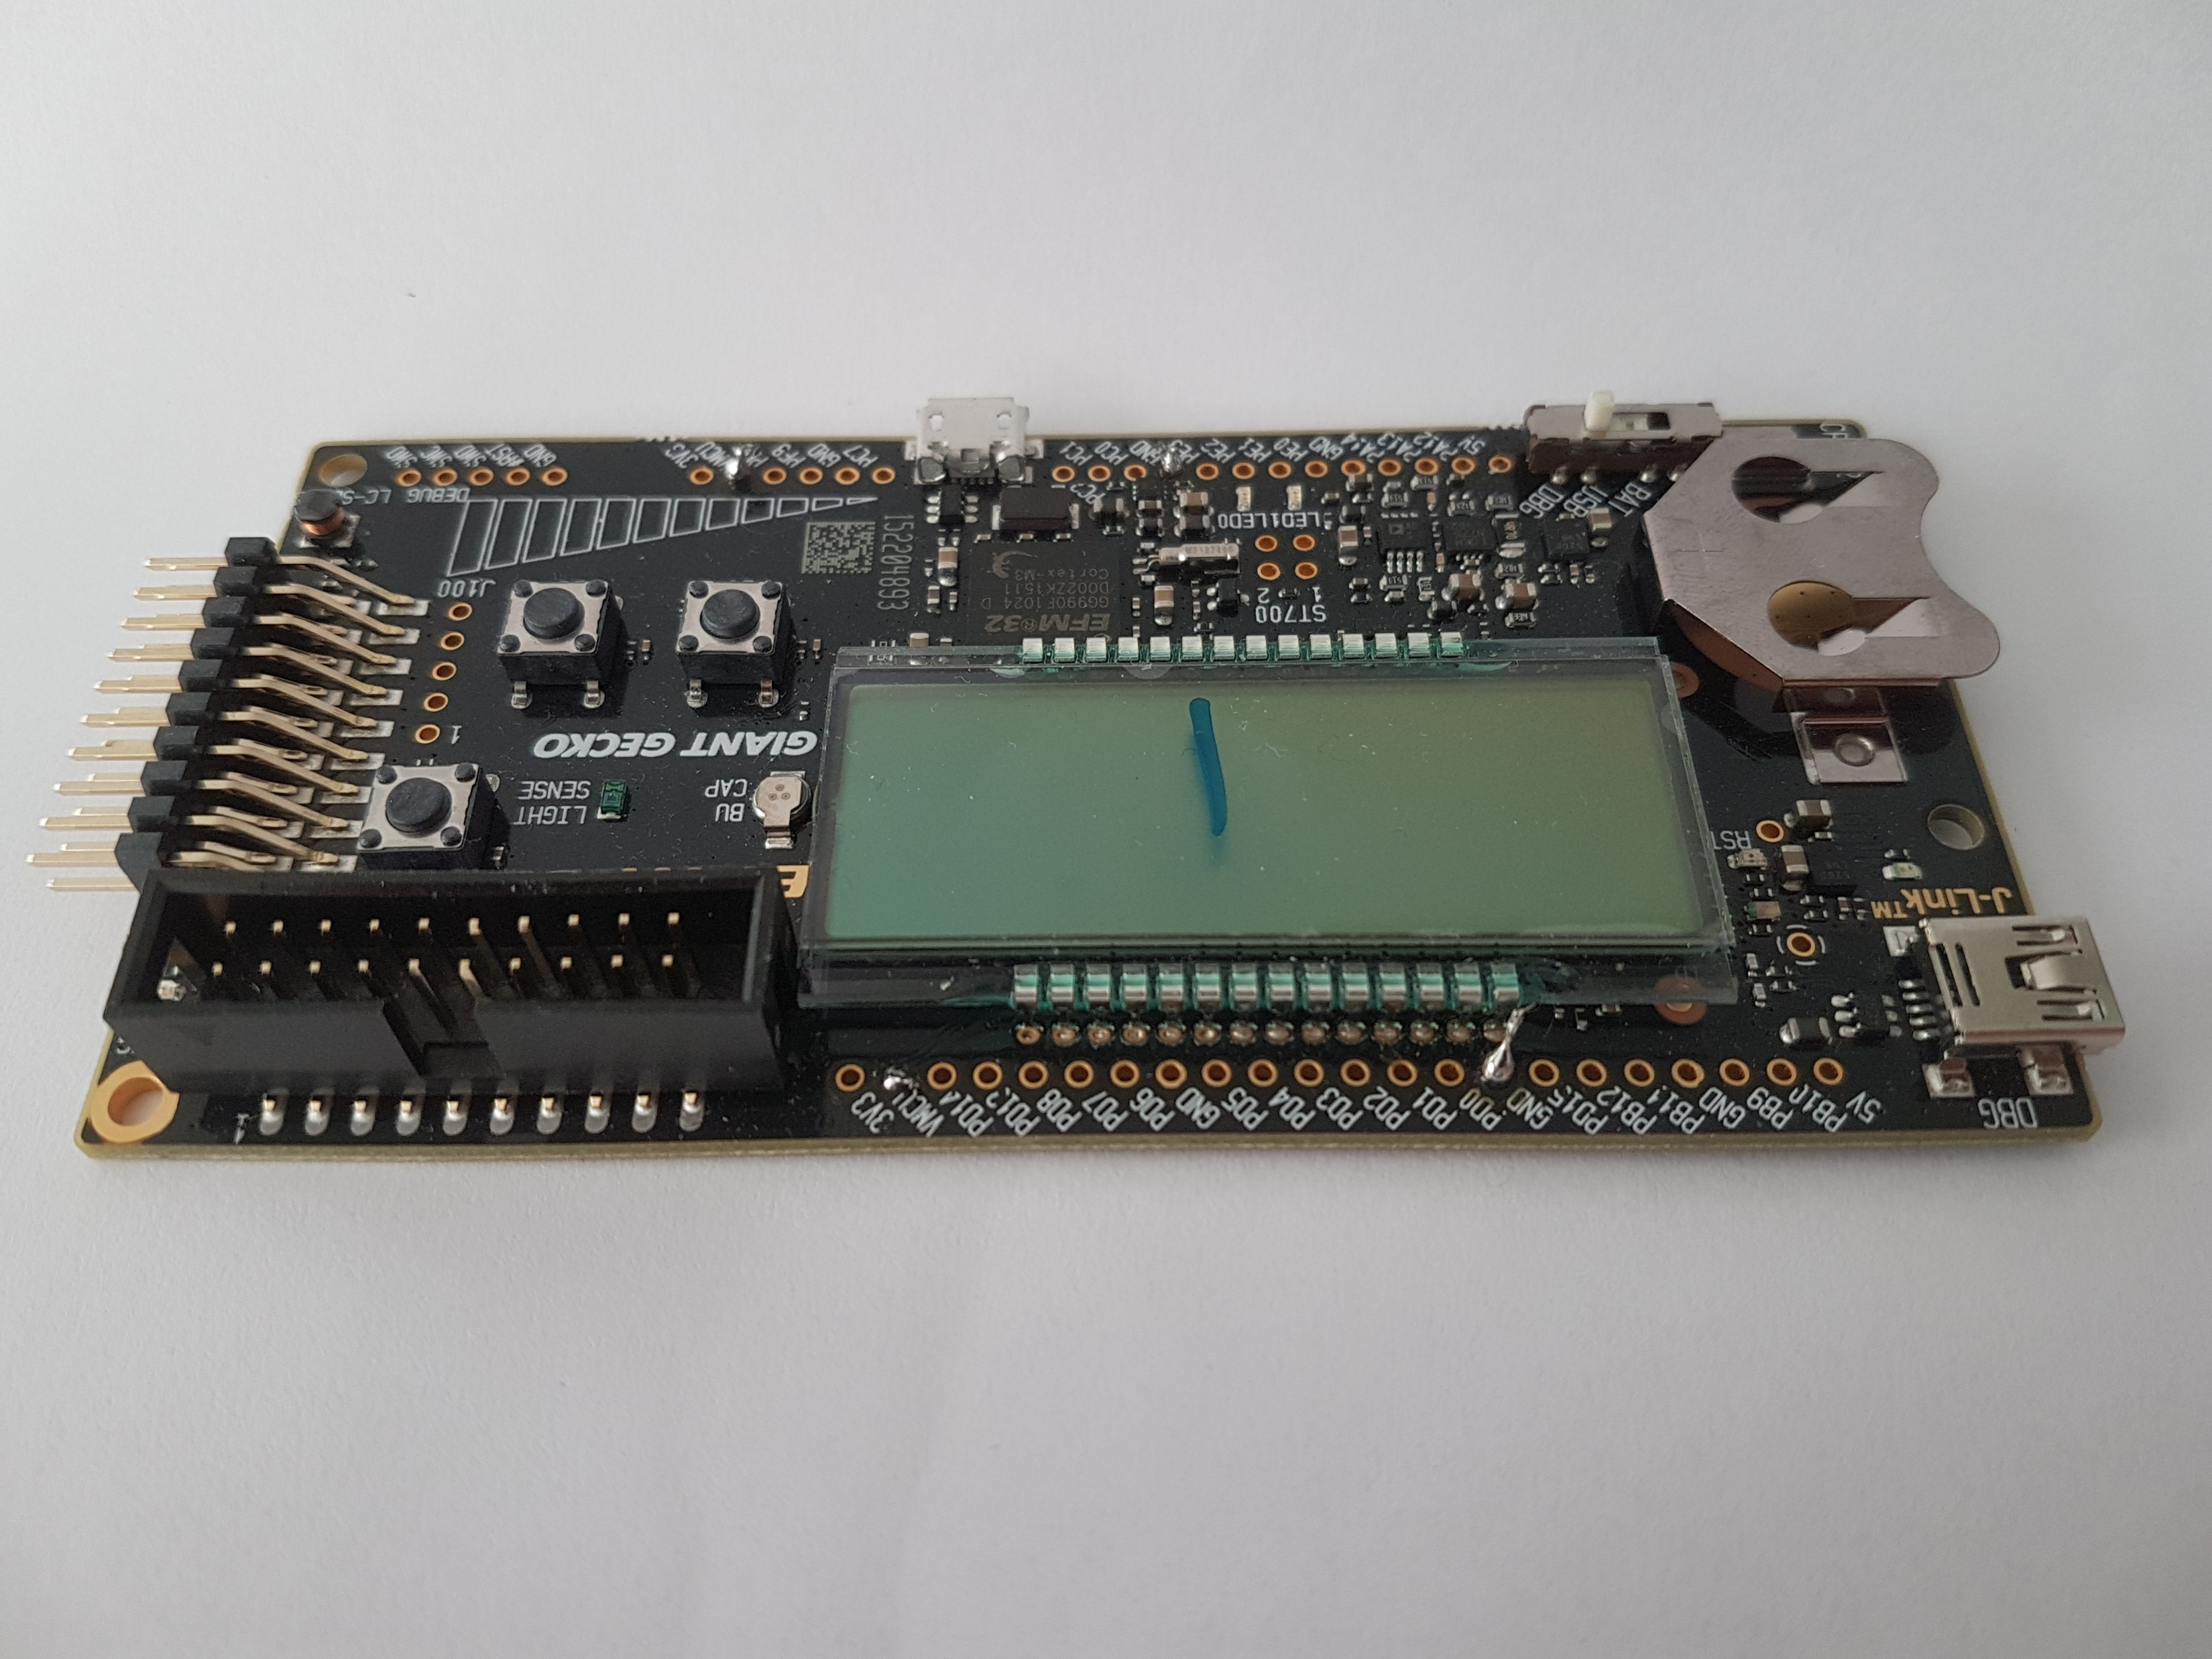
\includegraphics[width=.4\textwidth]{images/NFC8.jpg}}
\end{figure}
\begin{figure}
  \centering
  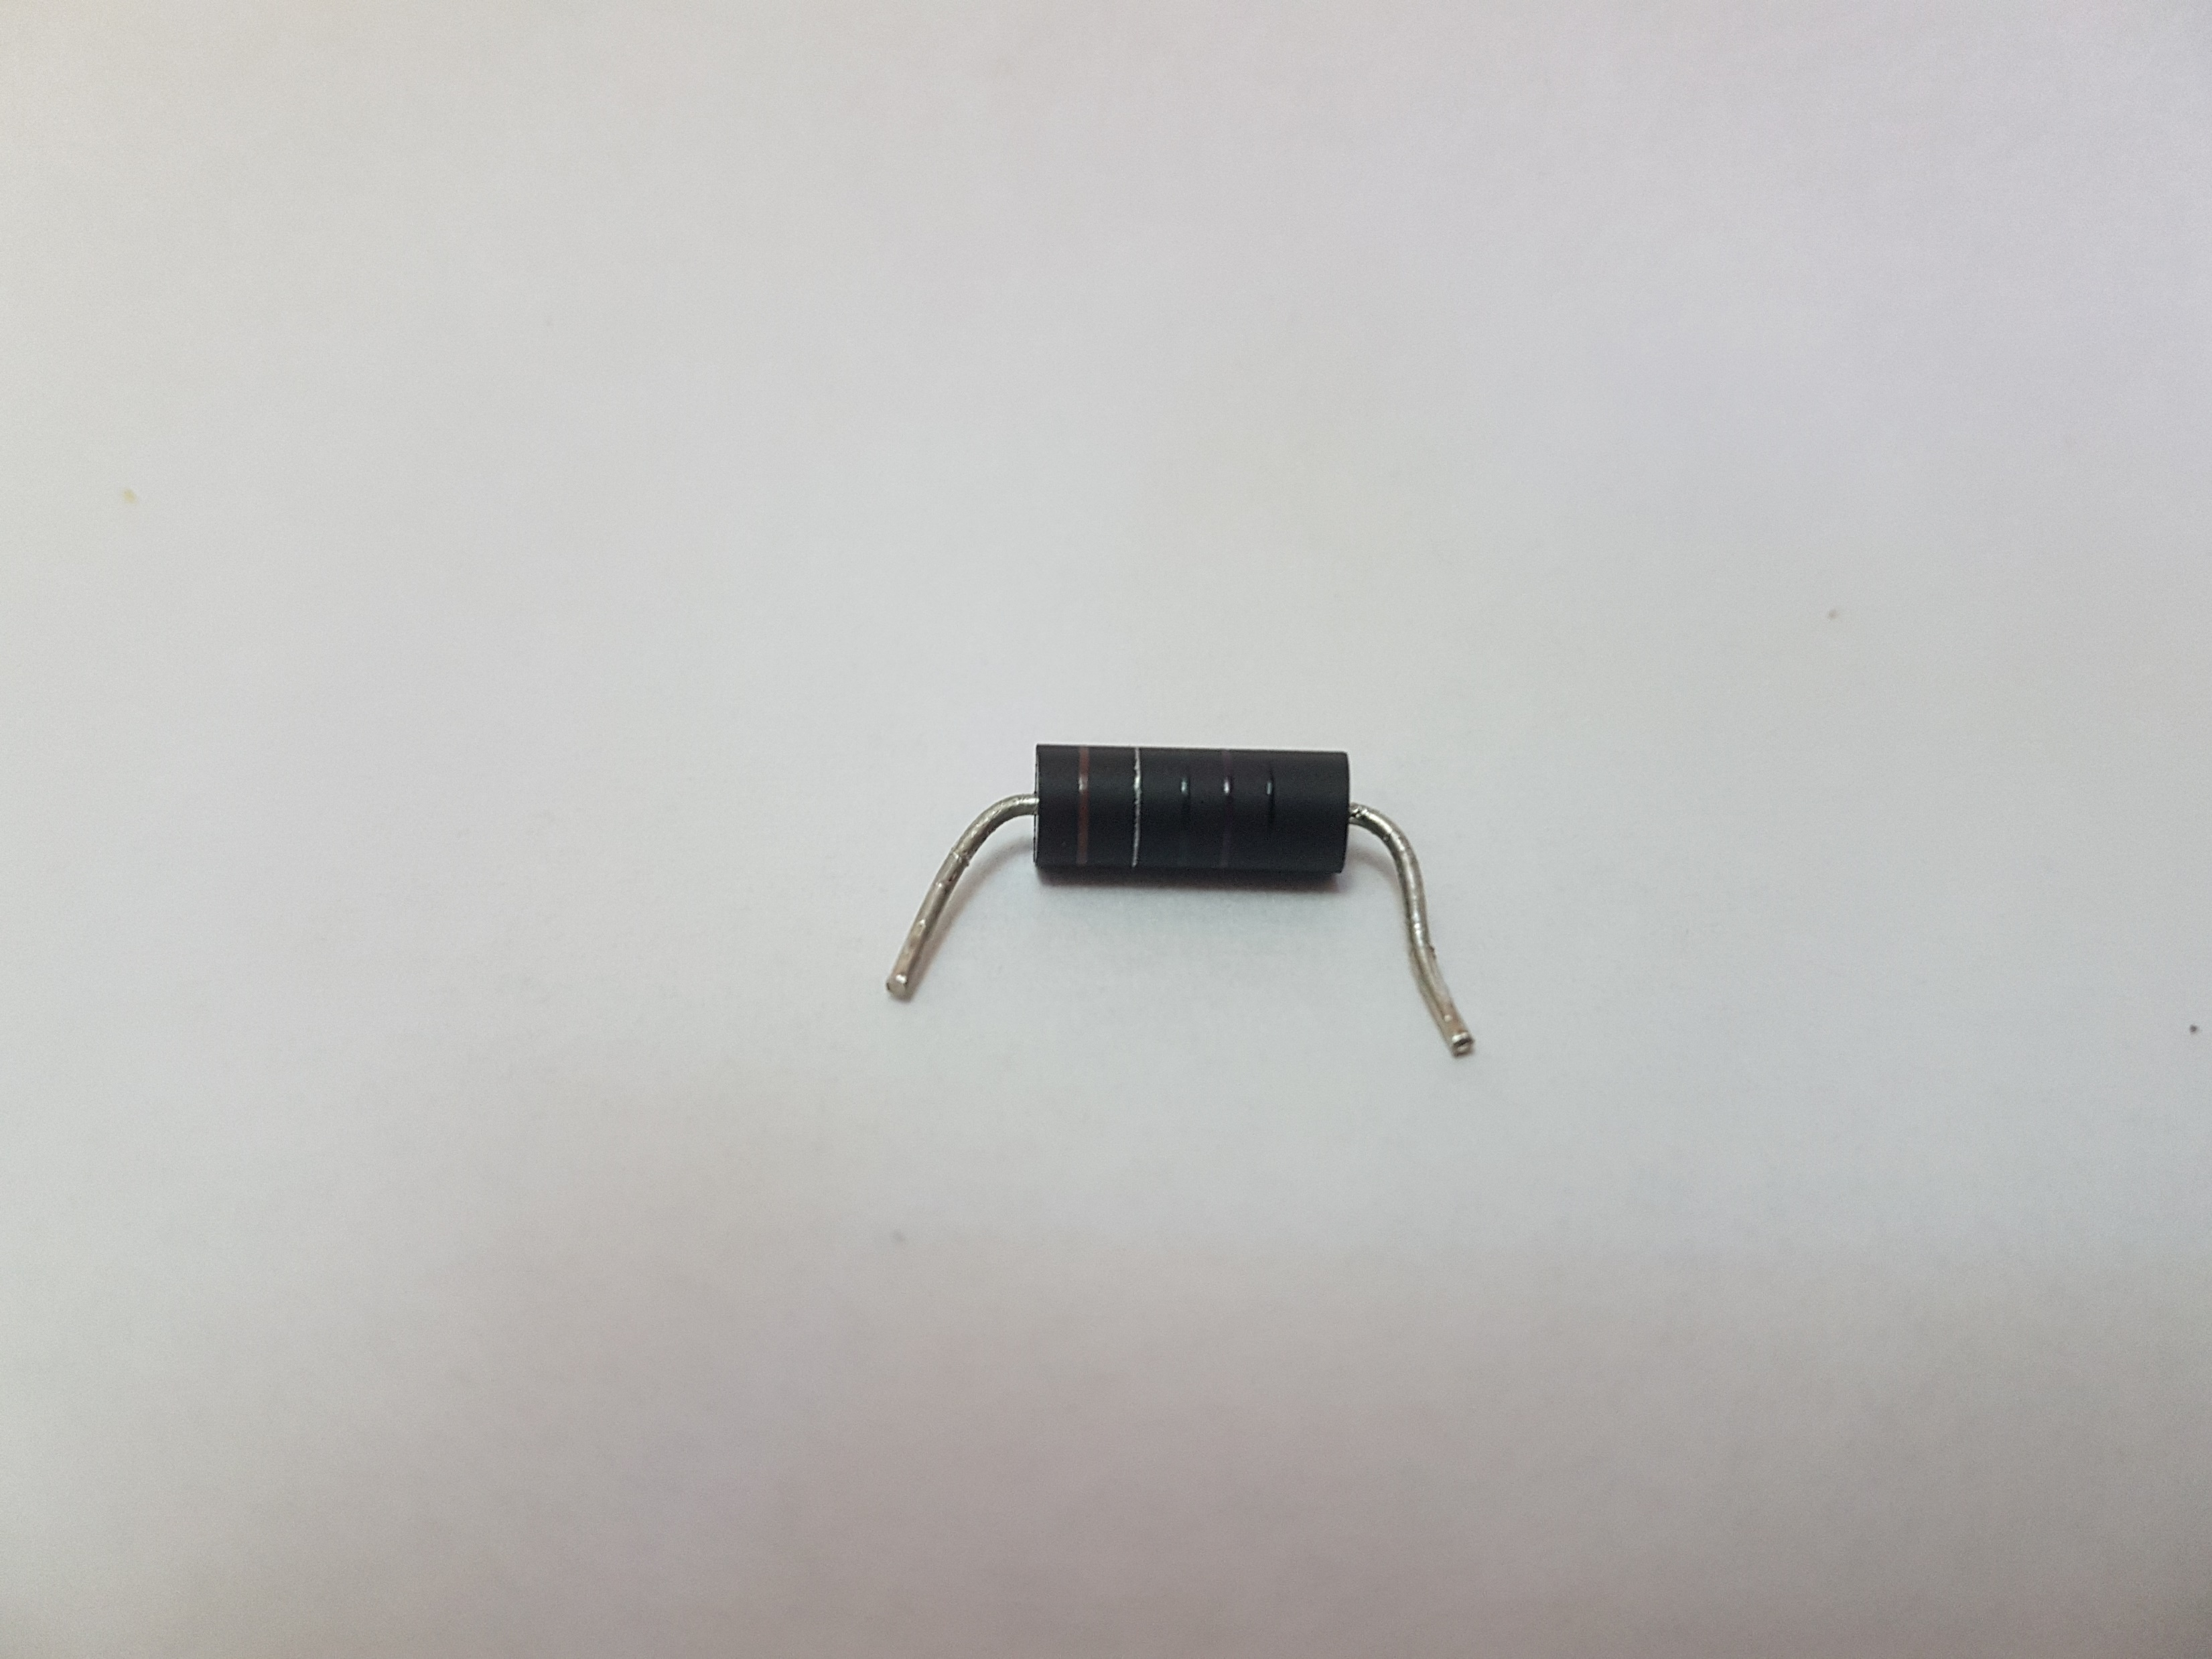
\includegraphics[width=.3\textwidth]{images/NFC9.jpg}
\end{figure}
\end{frame}

\begin{frame}[fragile]
\frametitle{NFC Node - Power Management} 
\begin{figure}
  \centering
  \subfloat{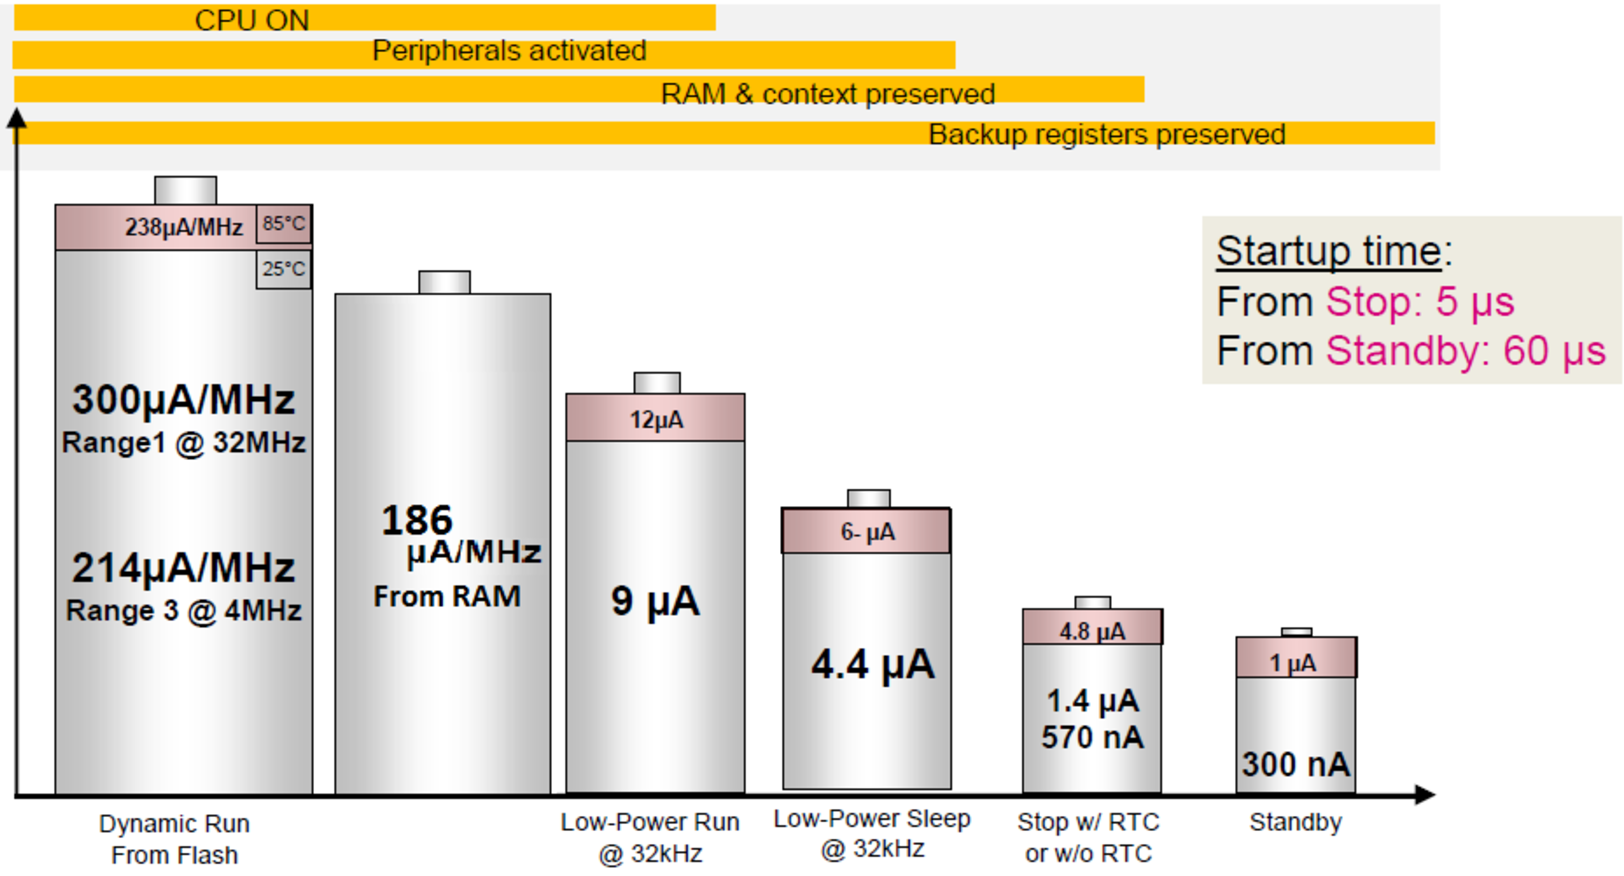
\includegraphics[width=.5\textwidth]{images/NFC10.png}}\qquad
  \subfloat{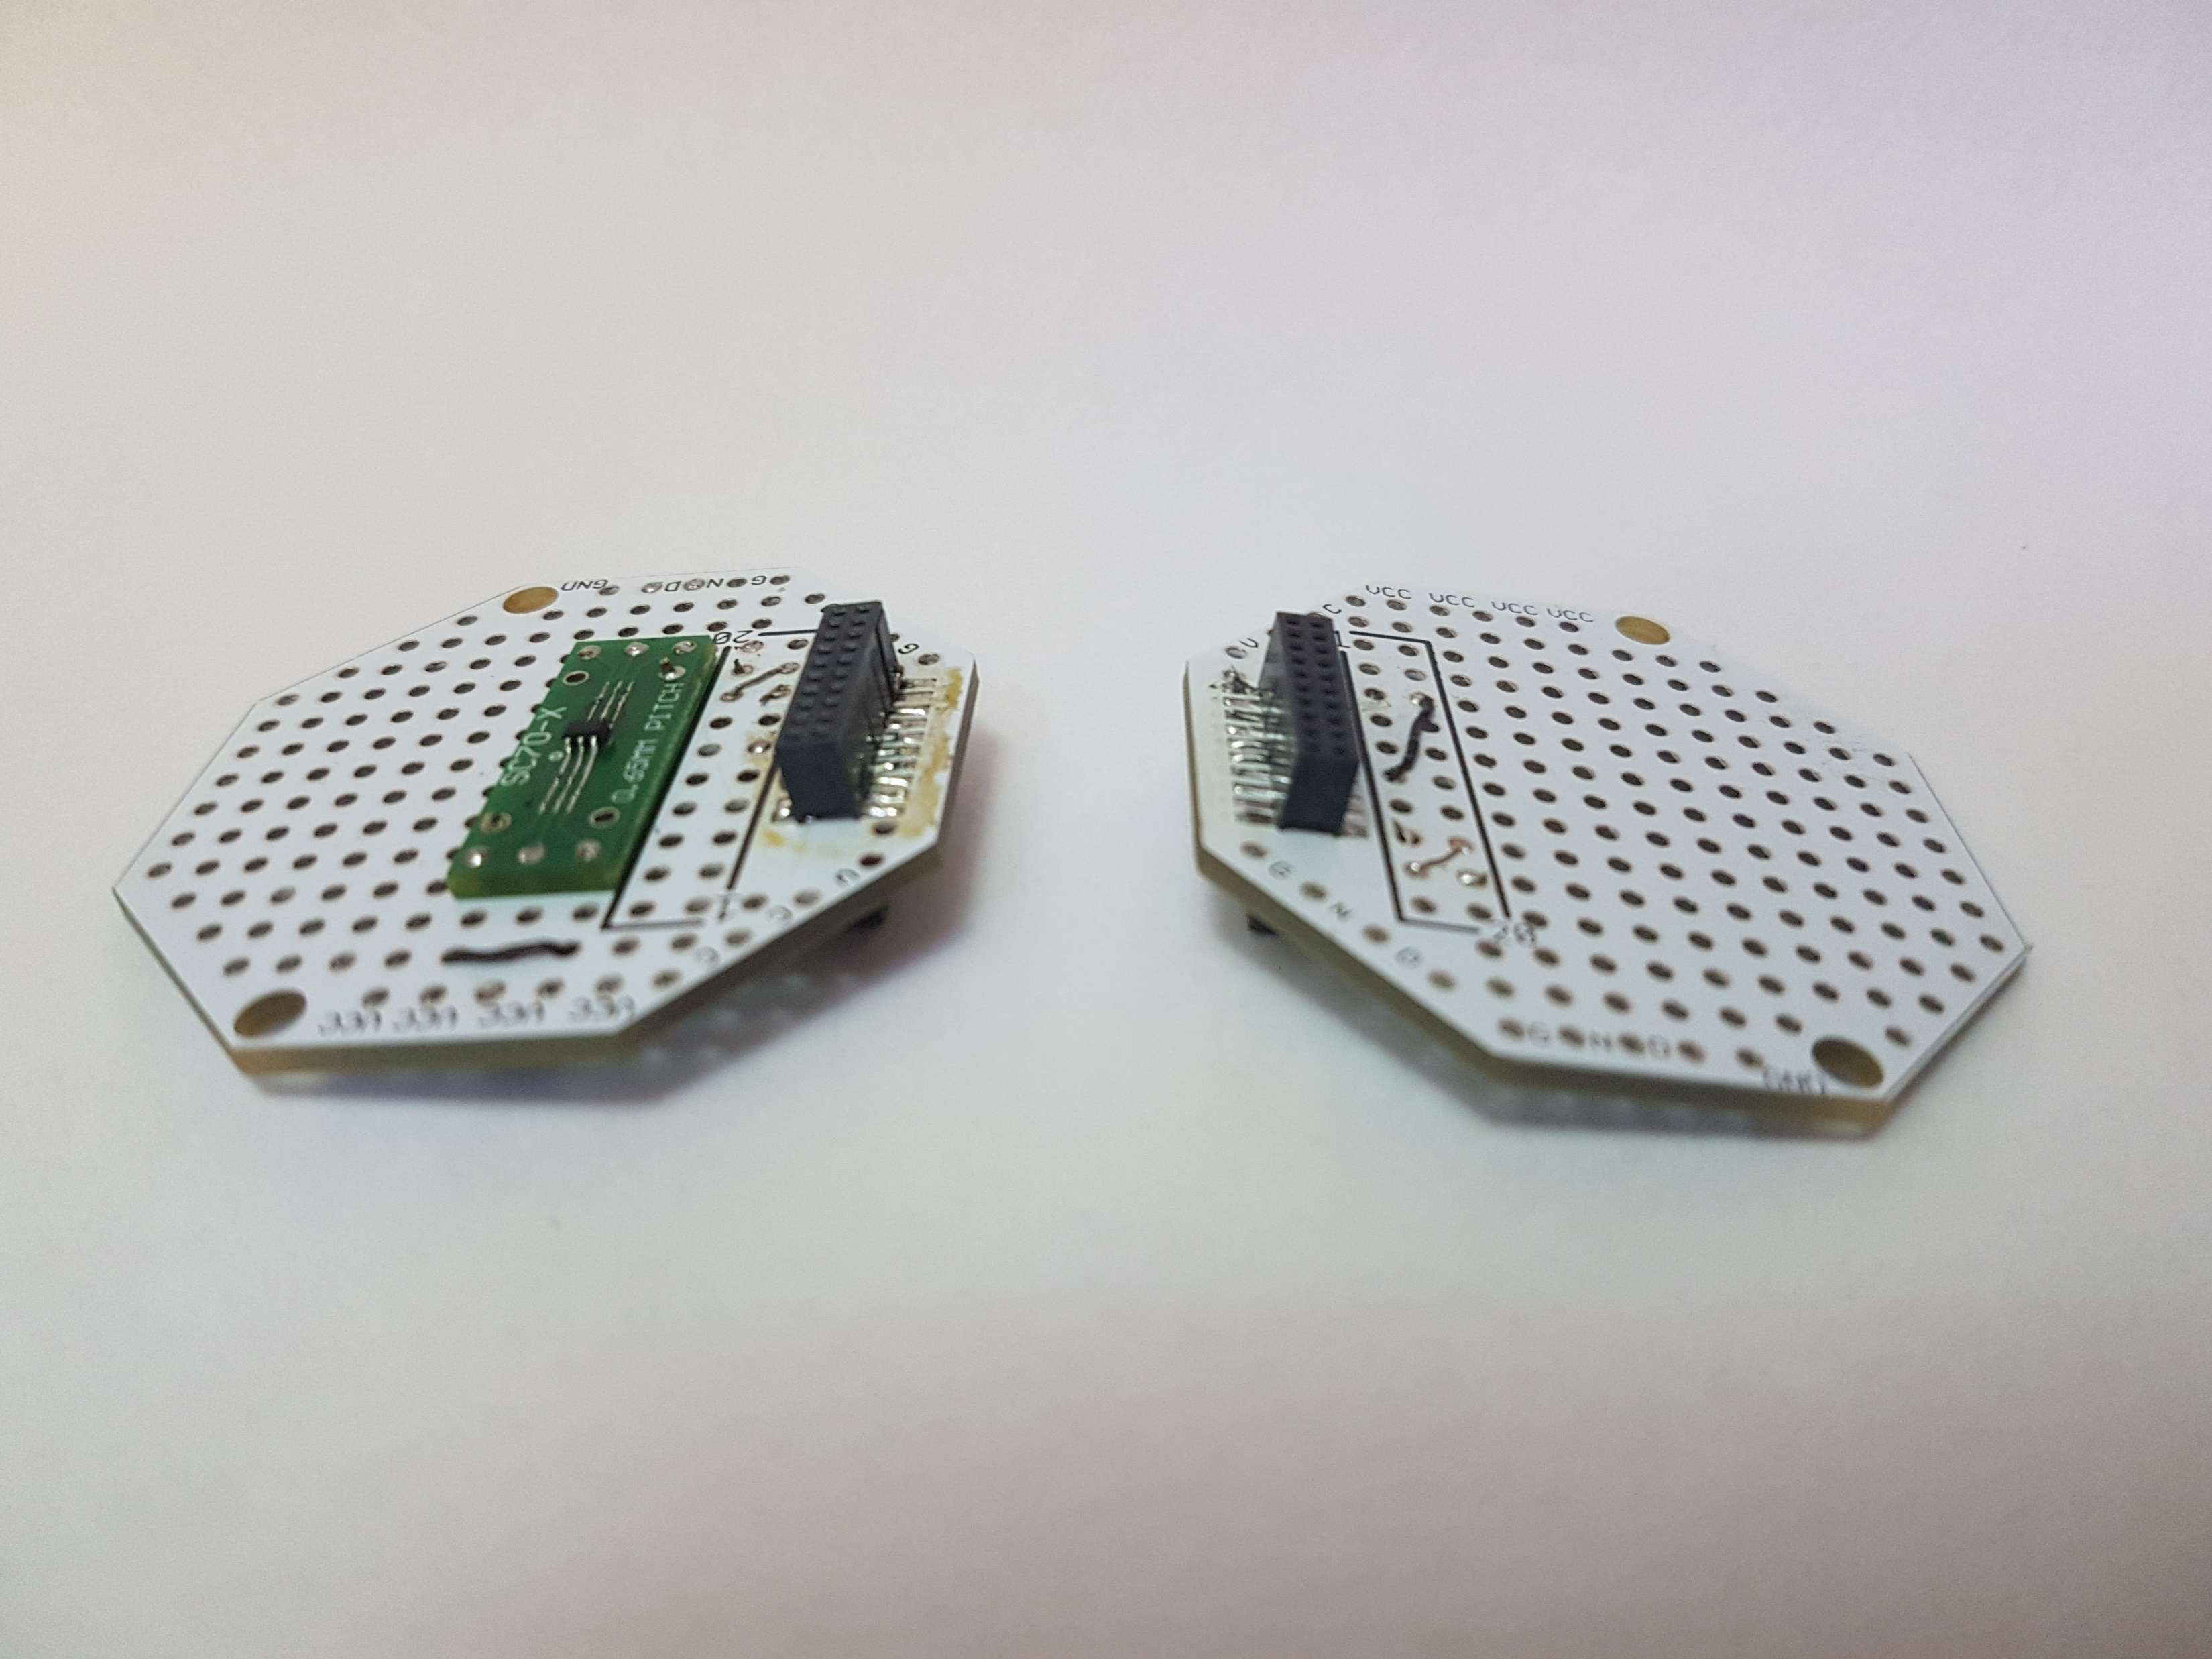
\includegraphics[width=.4\textwidth]{images/NFC11.jpg}}
\end{figure}
\end{frame}

\begin{frame}[fragile]
\frametitle{NFC Node - Power Management} 
\begin{figure}
  \centering
	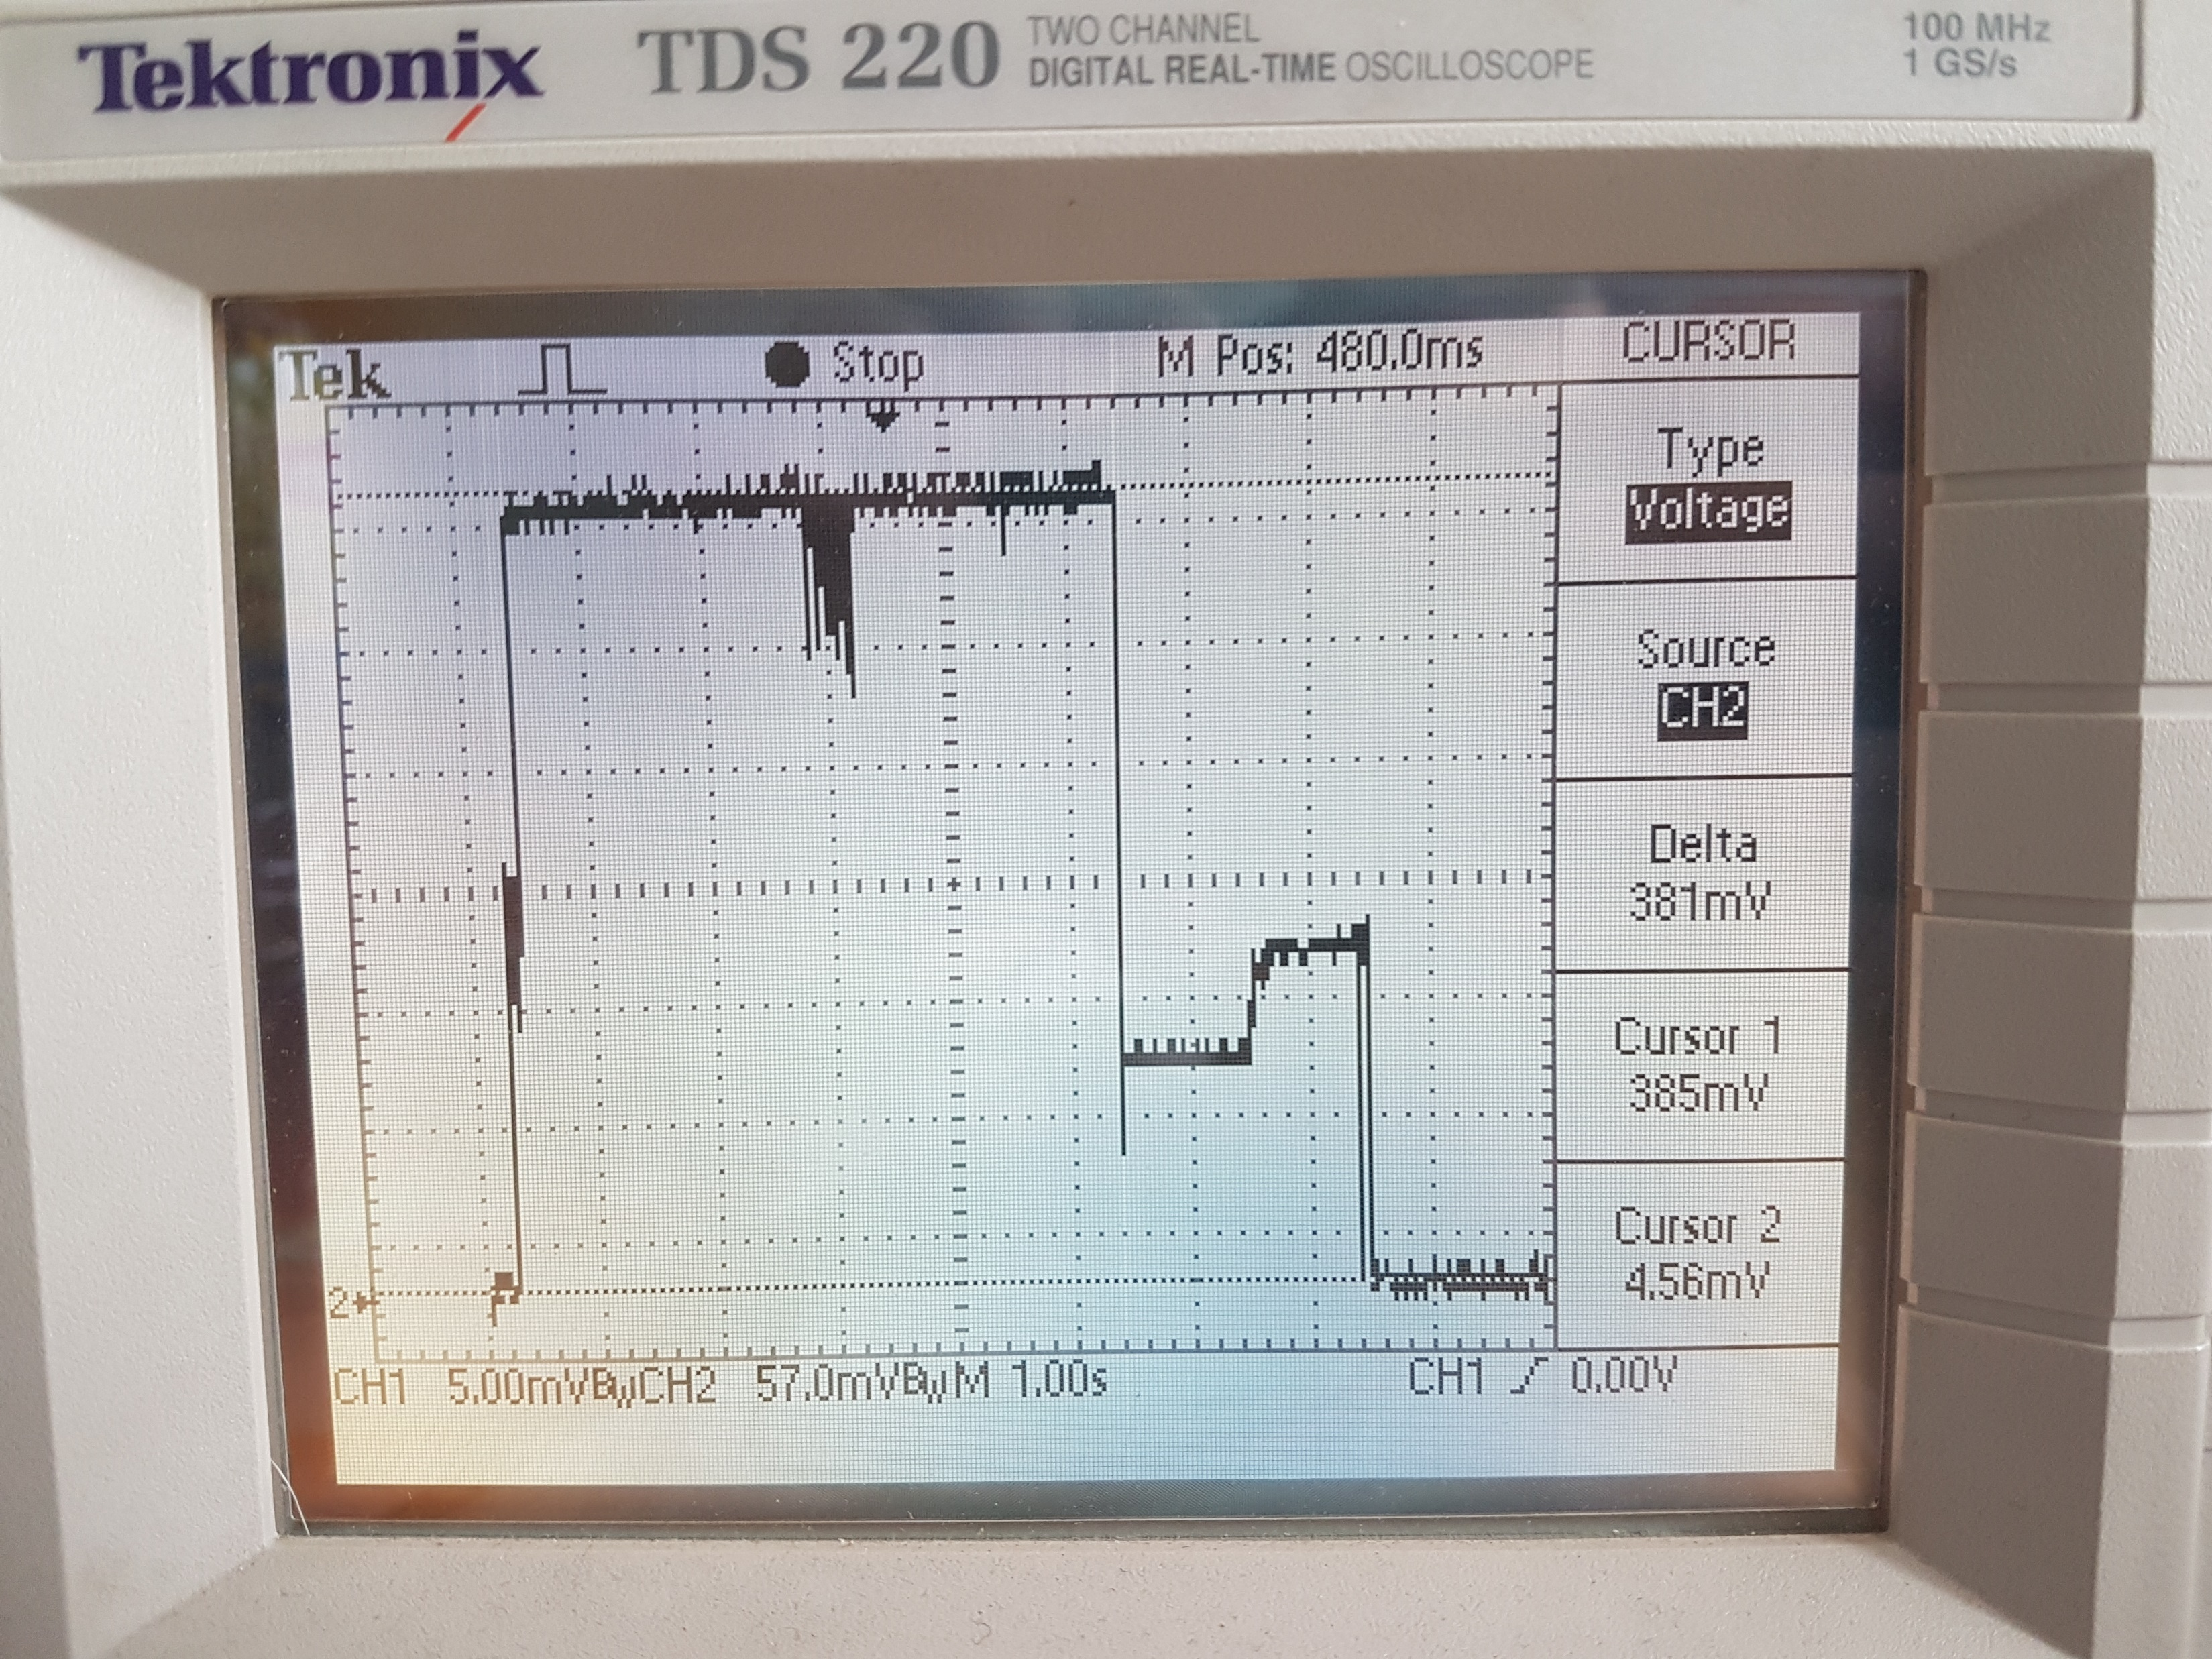
\includegraphics[width=\textwidth]{images/NFC12.jpg}
\end{figure}
\end{frame}

\begin{frame}[fragile]
\frametitle{NFC Node - Power Management} 
\begin{figure}
  \centering
	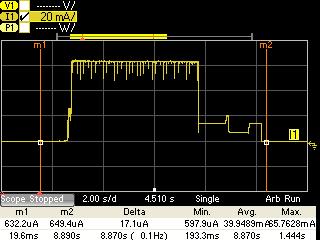
\includegraphics[width=\textwidth]{images/NFC13.jpg}
\end{figure}
\end{frame}

\begin{frame}[fragile]
\frametitle{NFC Node - Power Management} 
\begin{figure}
  \centering
  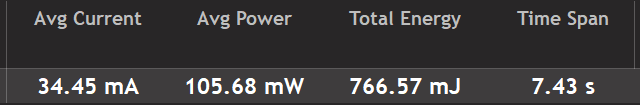
\includegraphics[width=.5\textwidth]{images/NFC16.png} \\
	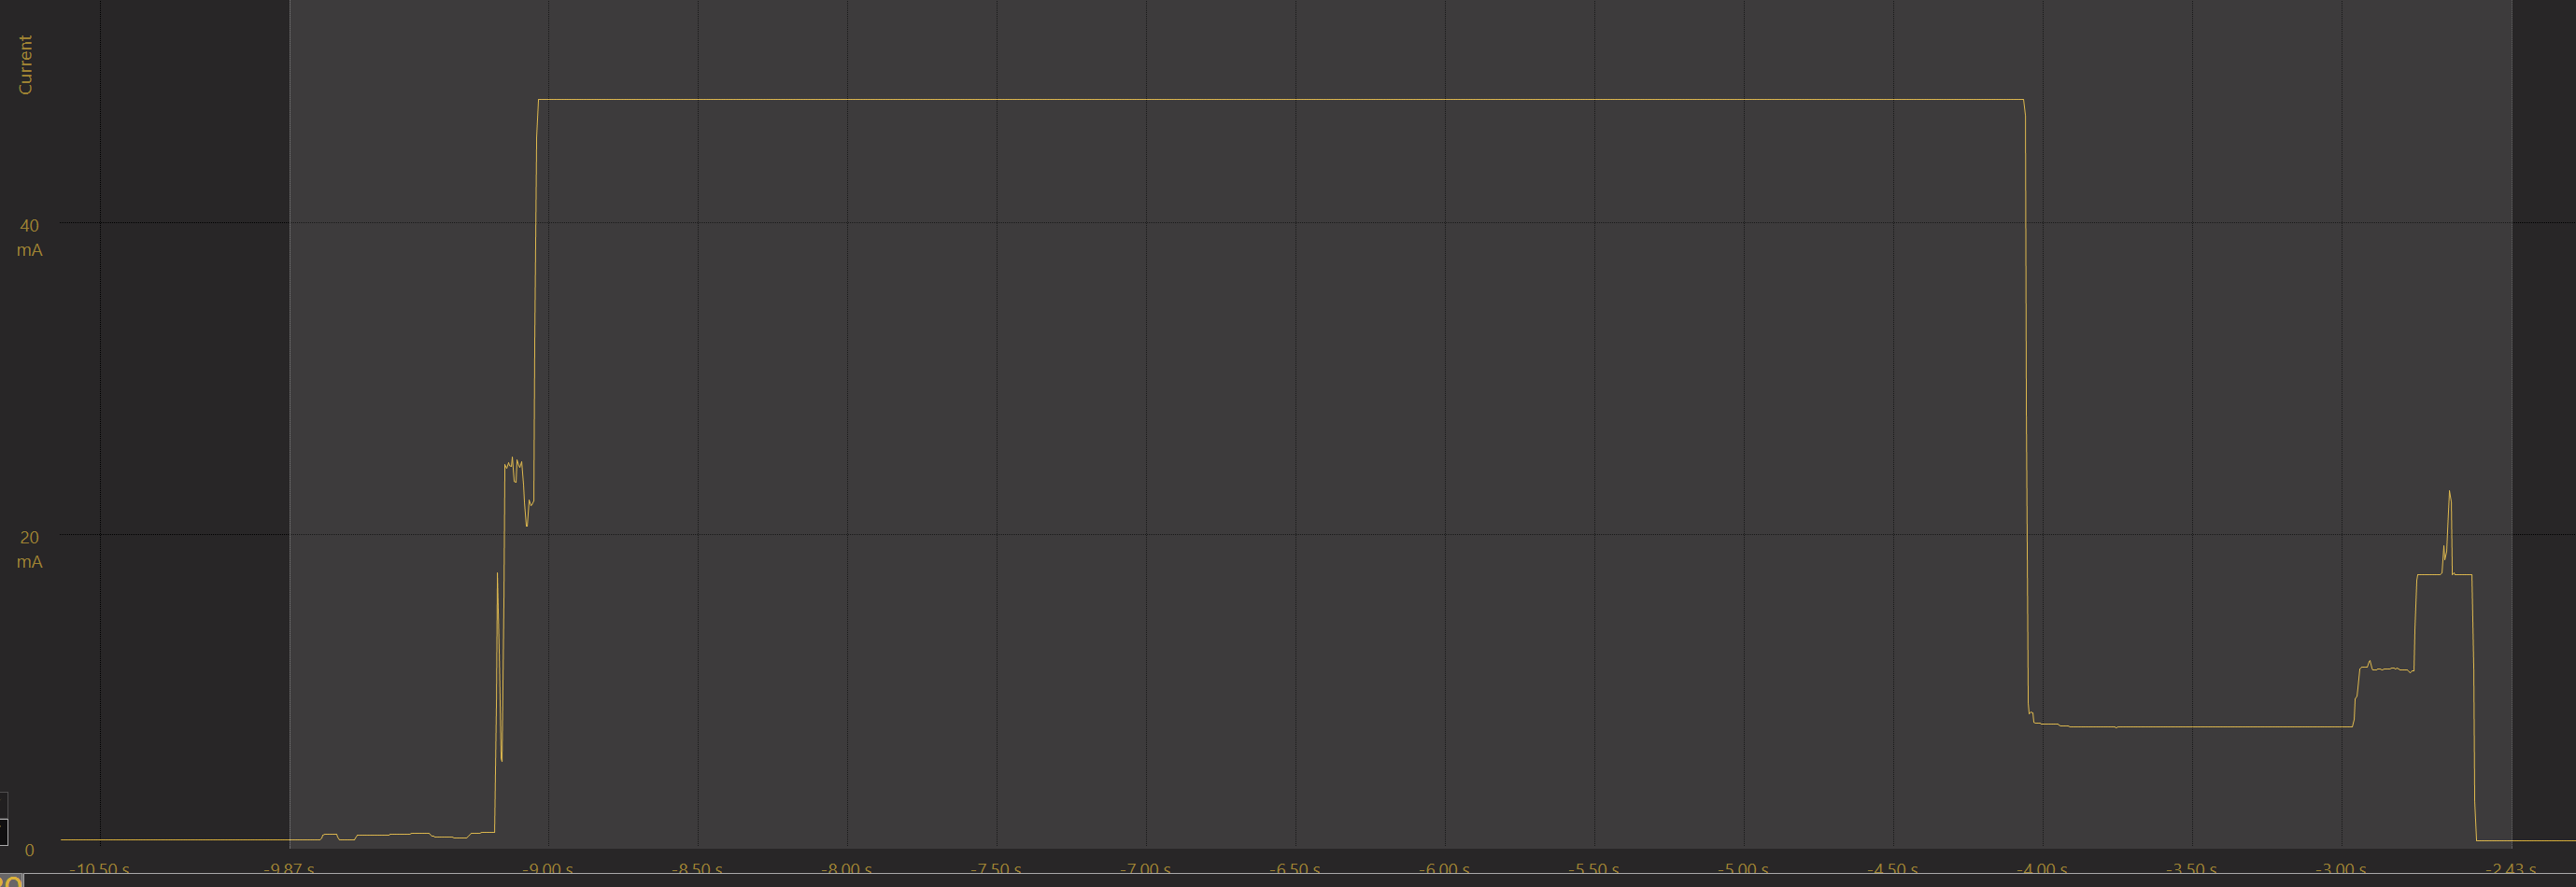
\includegraphics[width=\textwidth]{images/NFC14.png}
\end{figure}
\end{frame}

\begin{frame}[fragile]
\frametitle{NFC Node - Power Management} 
\begin{figure}
  \centering
	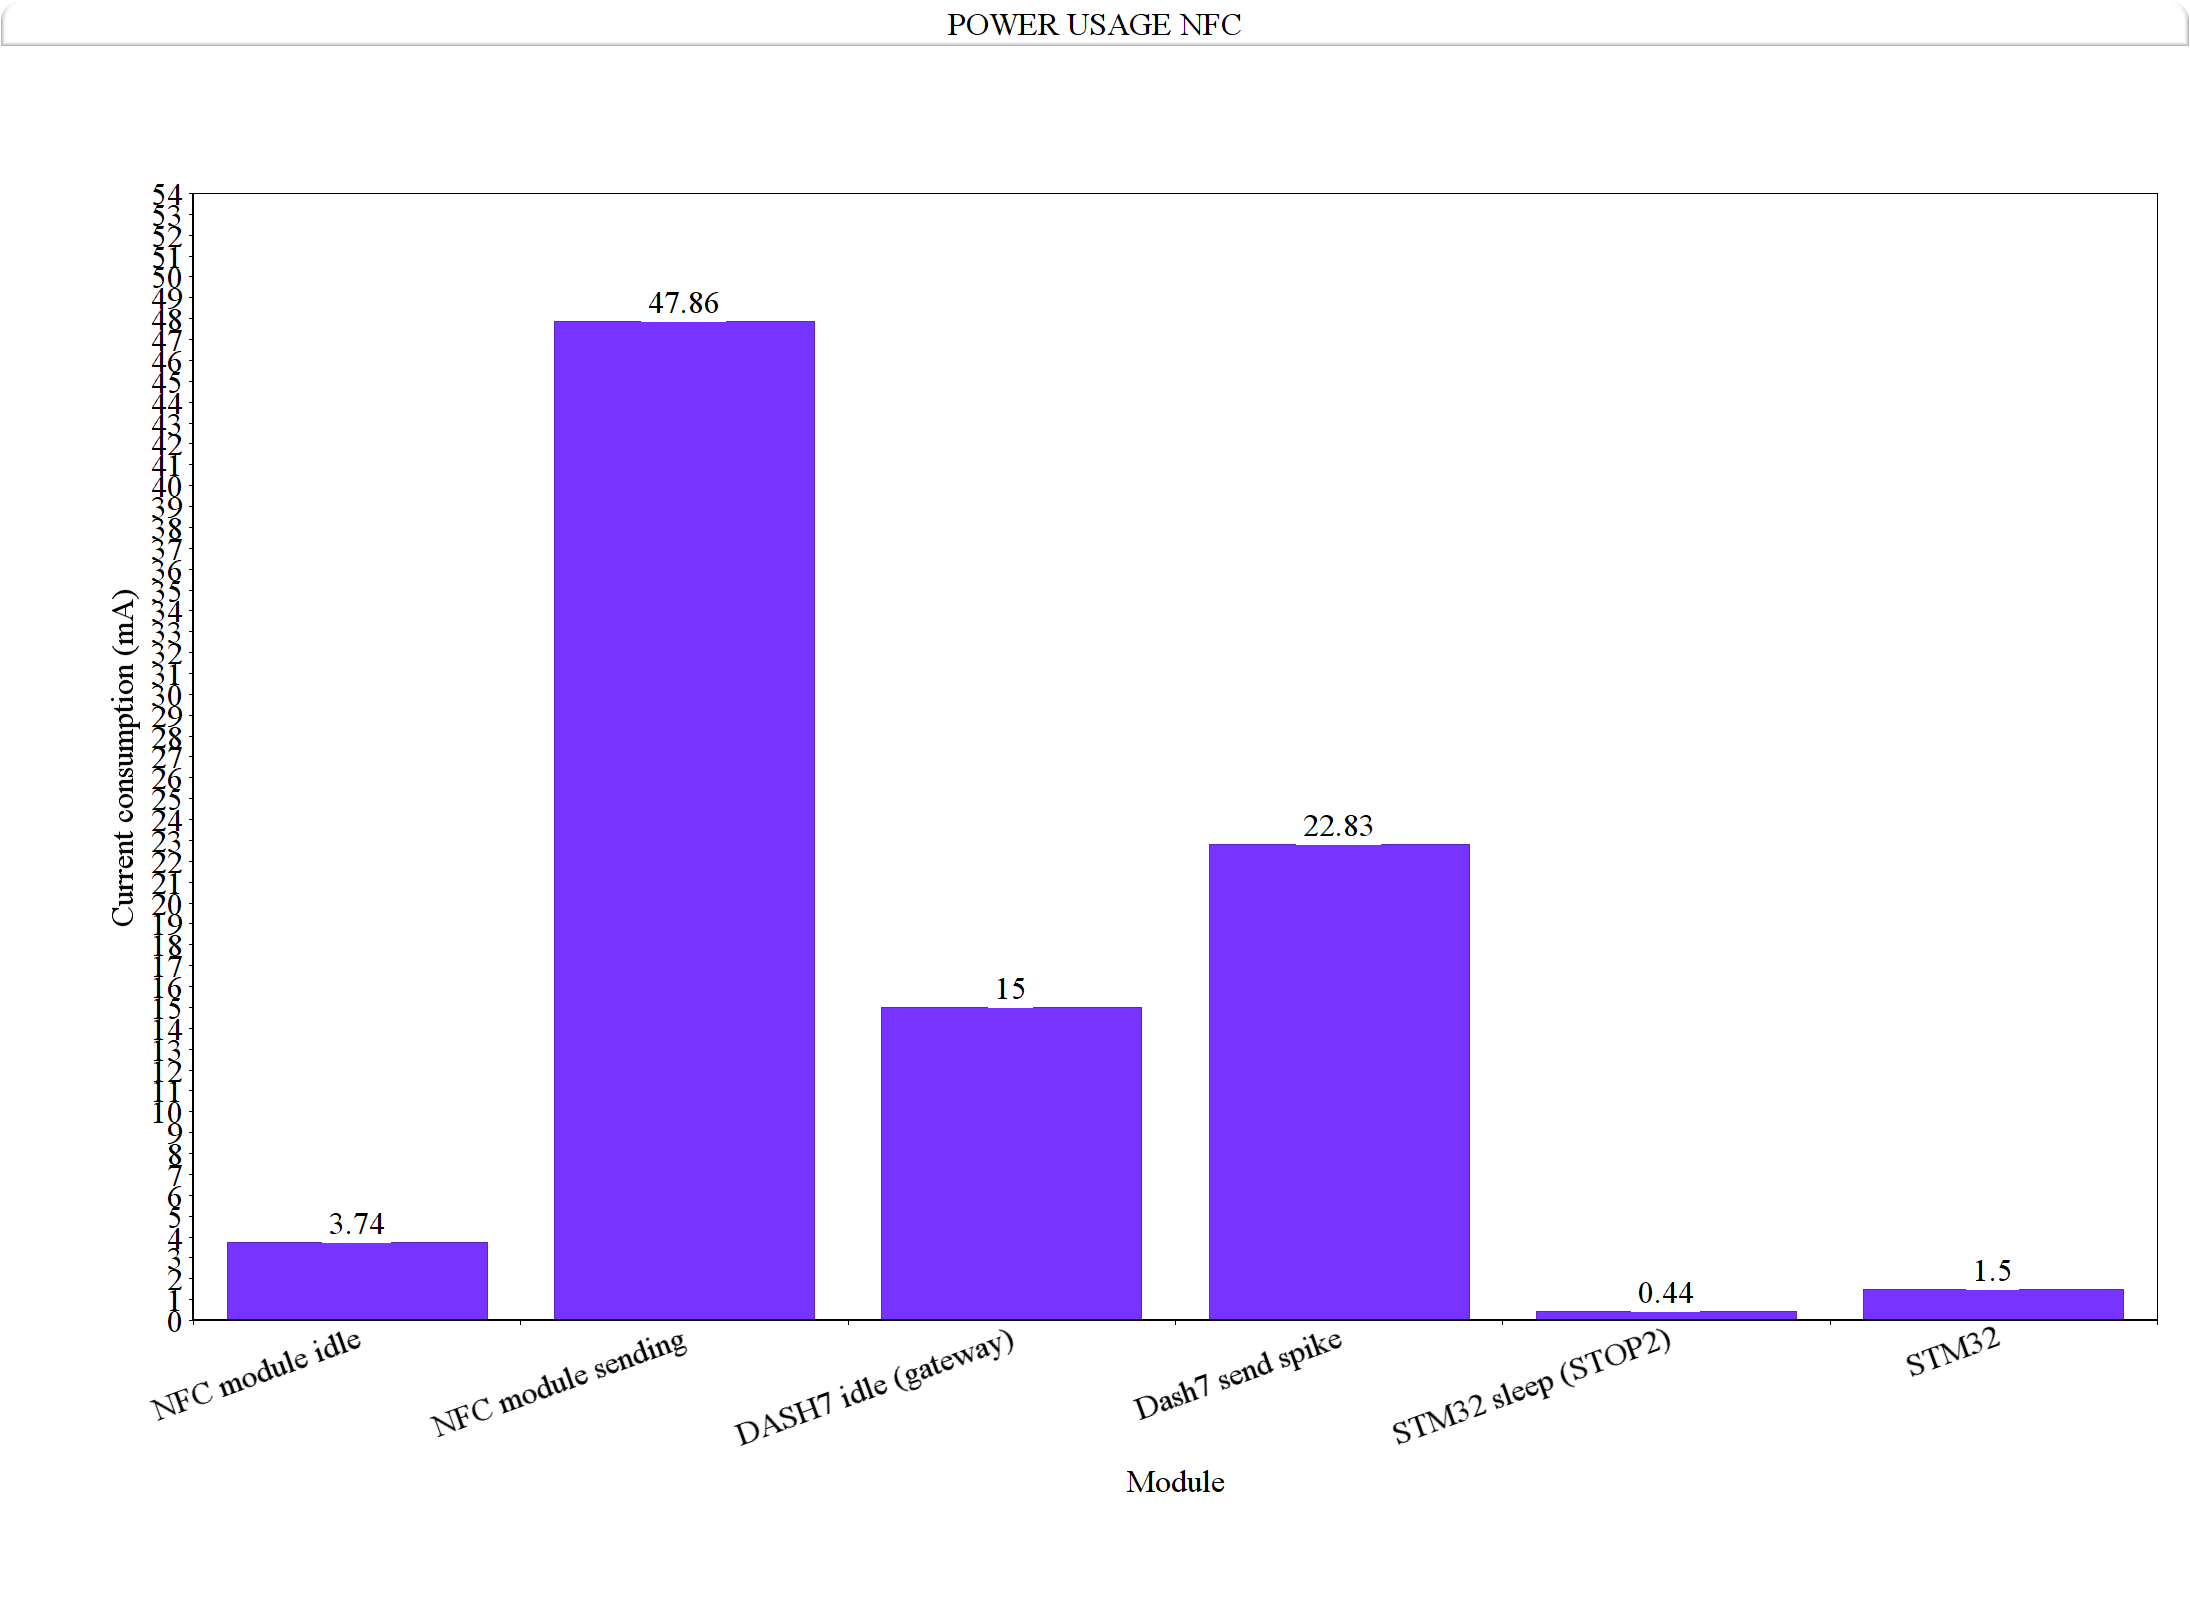
\includegraphics[width=\textwidth]{images/NFC15.png}
\end{figure}
\end{frame}


\subsection{Mobile Node}

\begin{frame}[fragile]
\frametitle{Mobile Node - Hardware} 
\begin{figure}
  \centering
  \subfloat{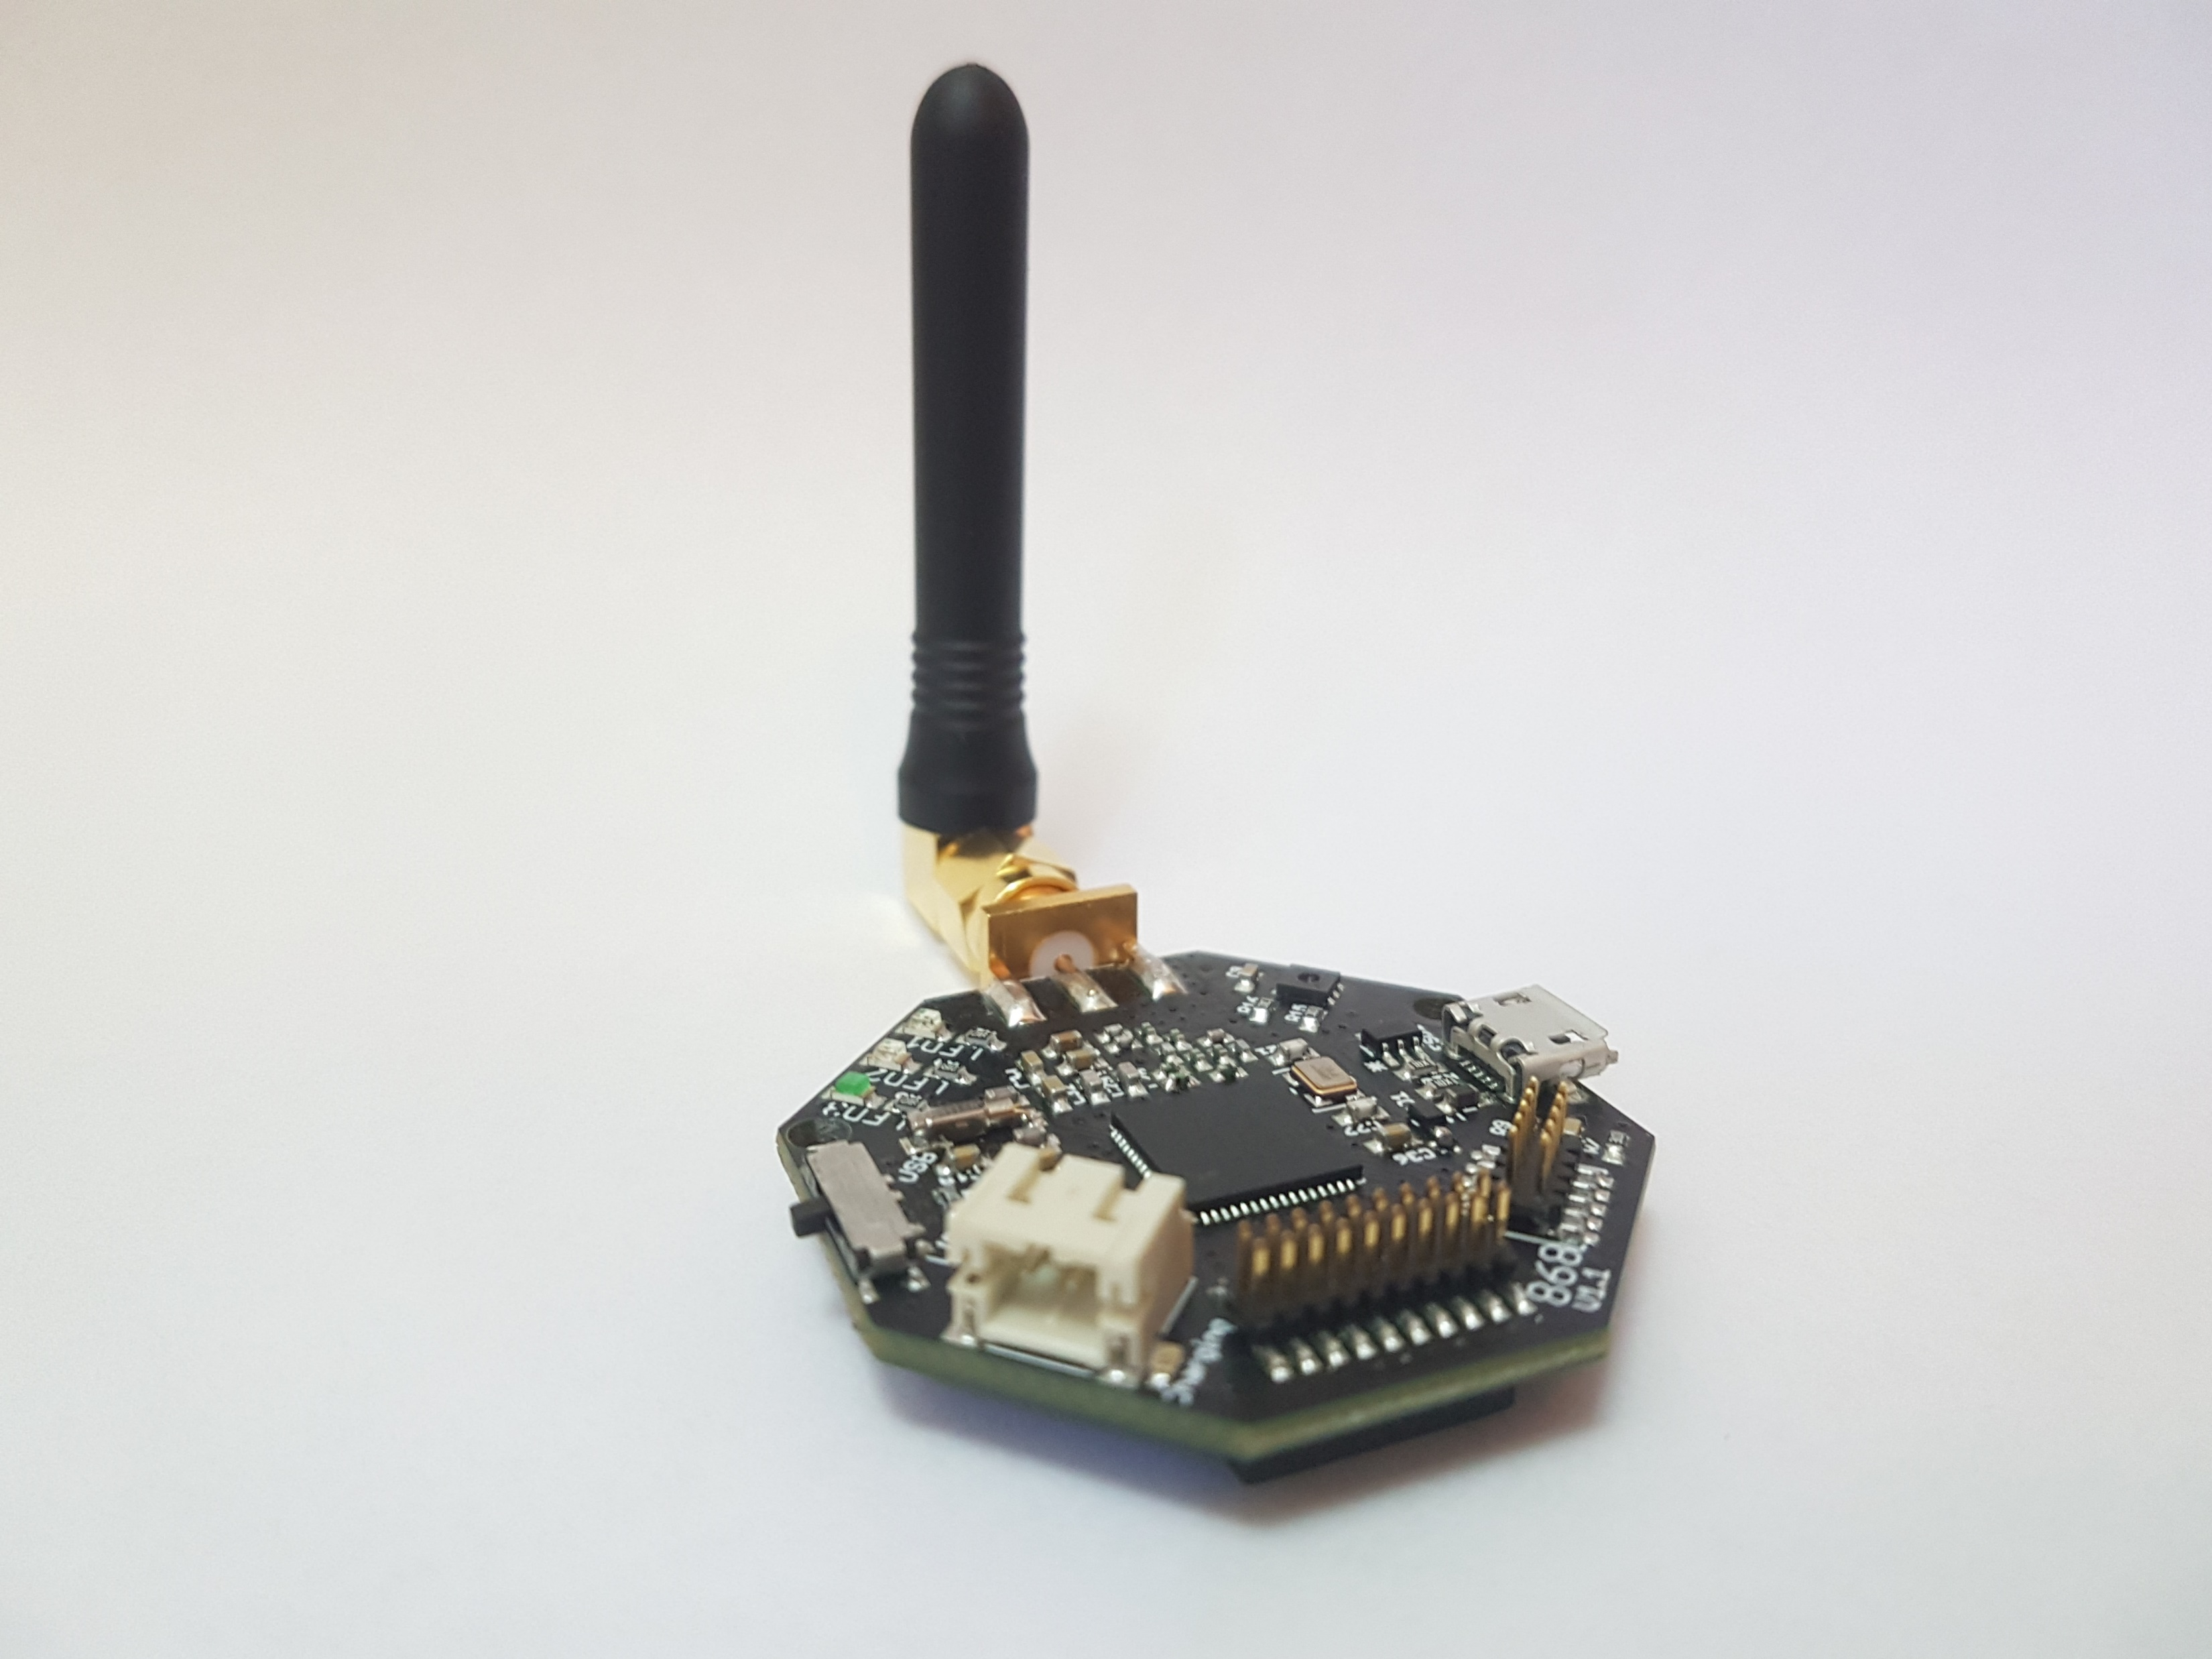
\includegraphics[width=.4\textwidth]{images/mobile1.jpg}}\qquad
  \subfloat{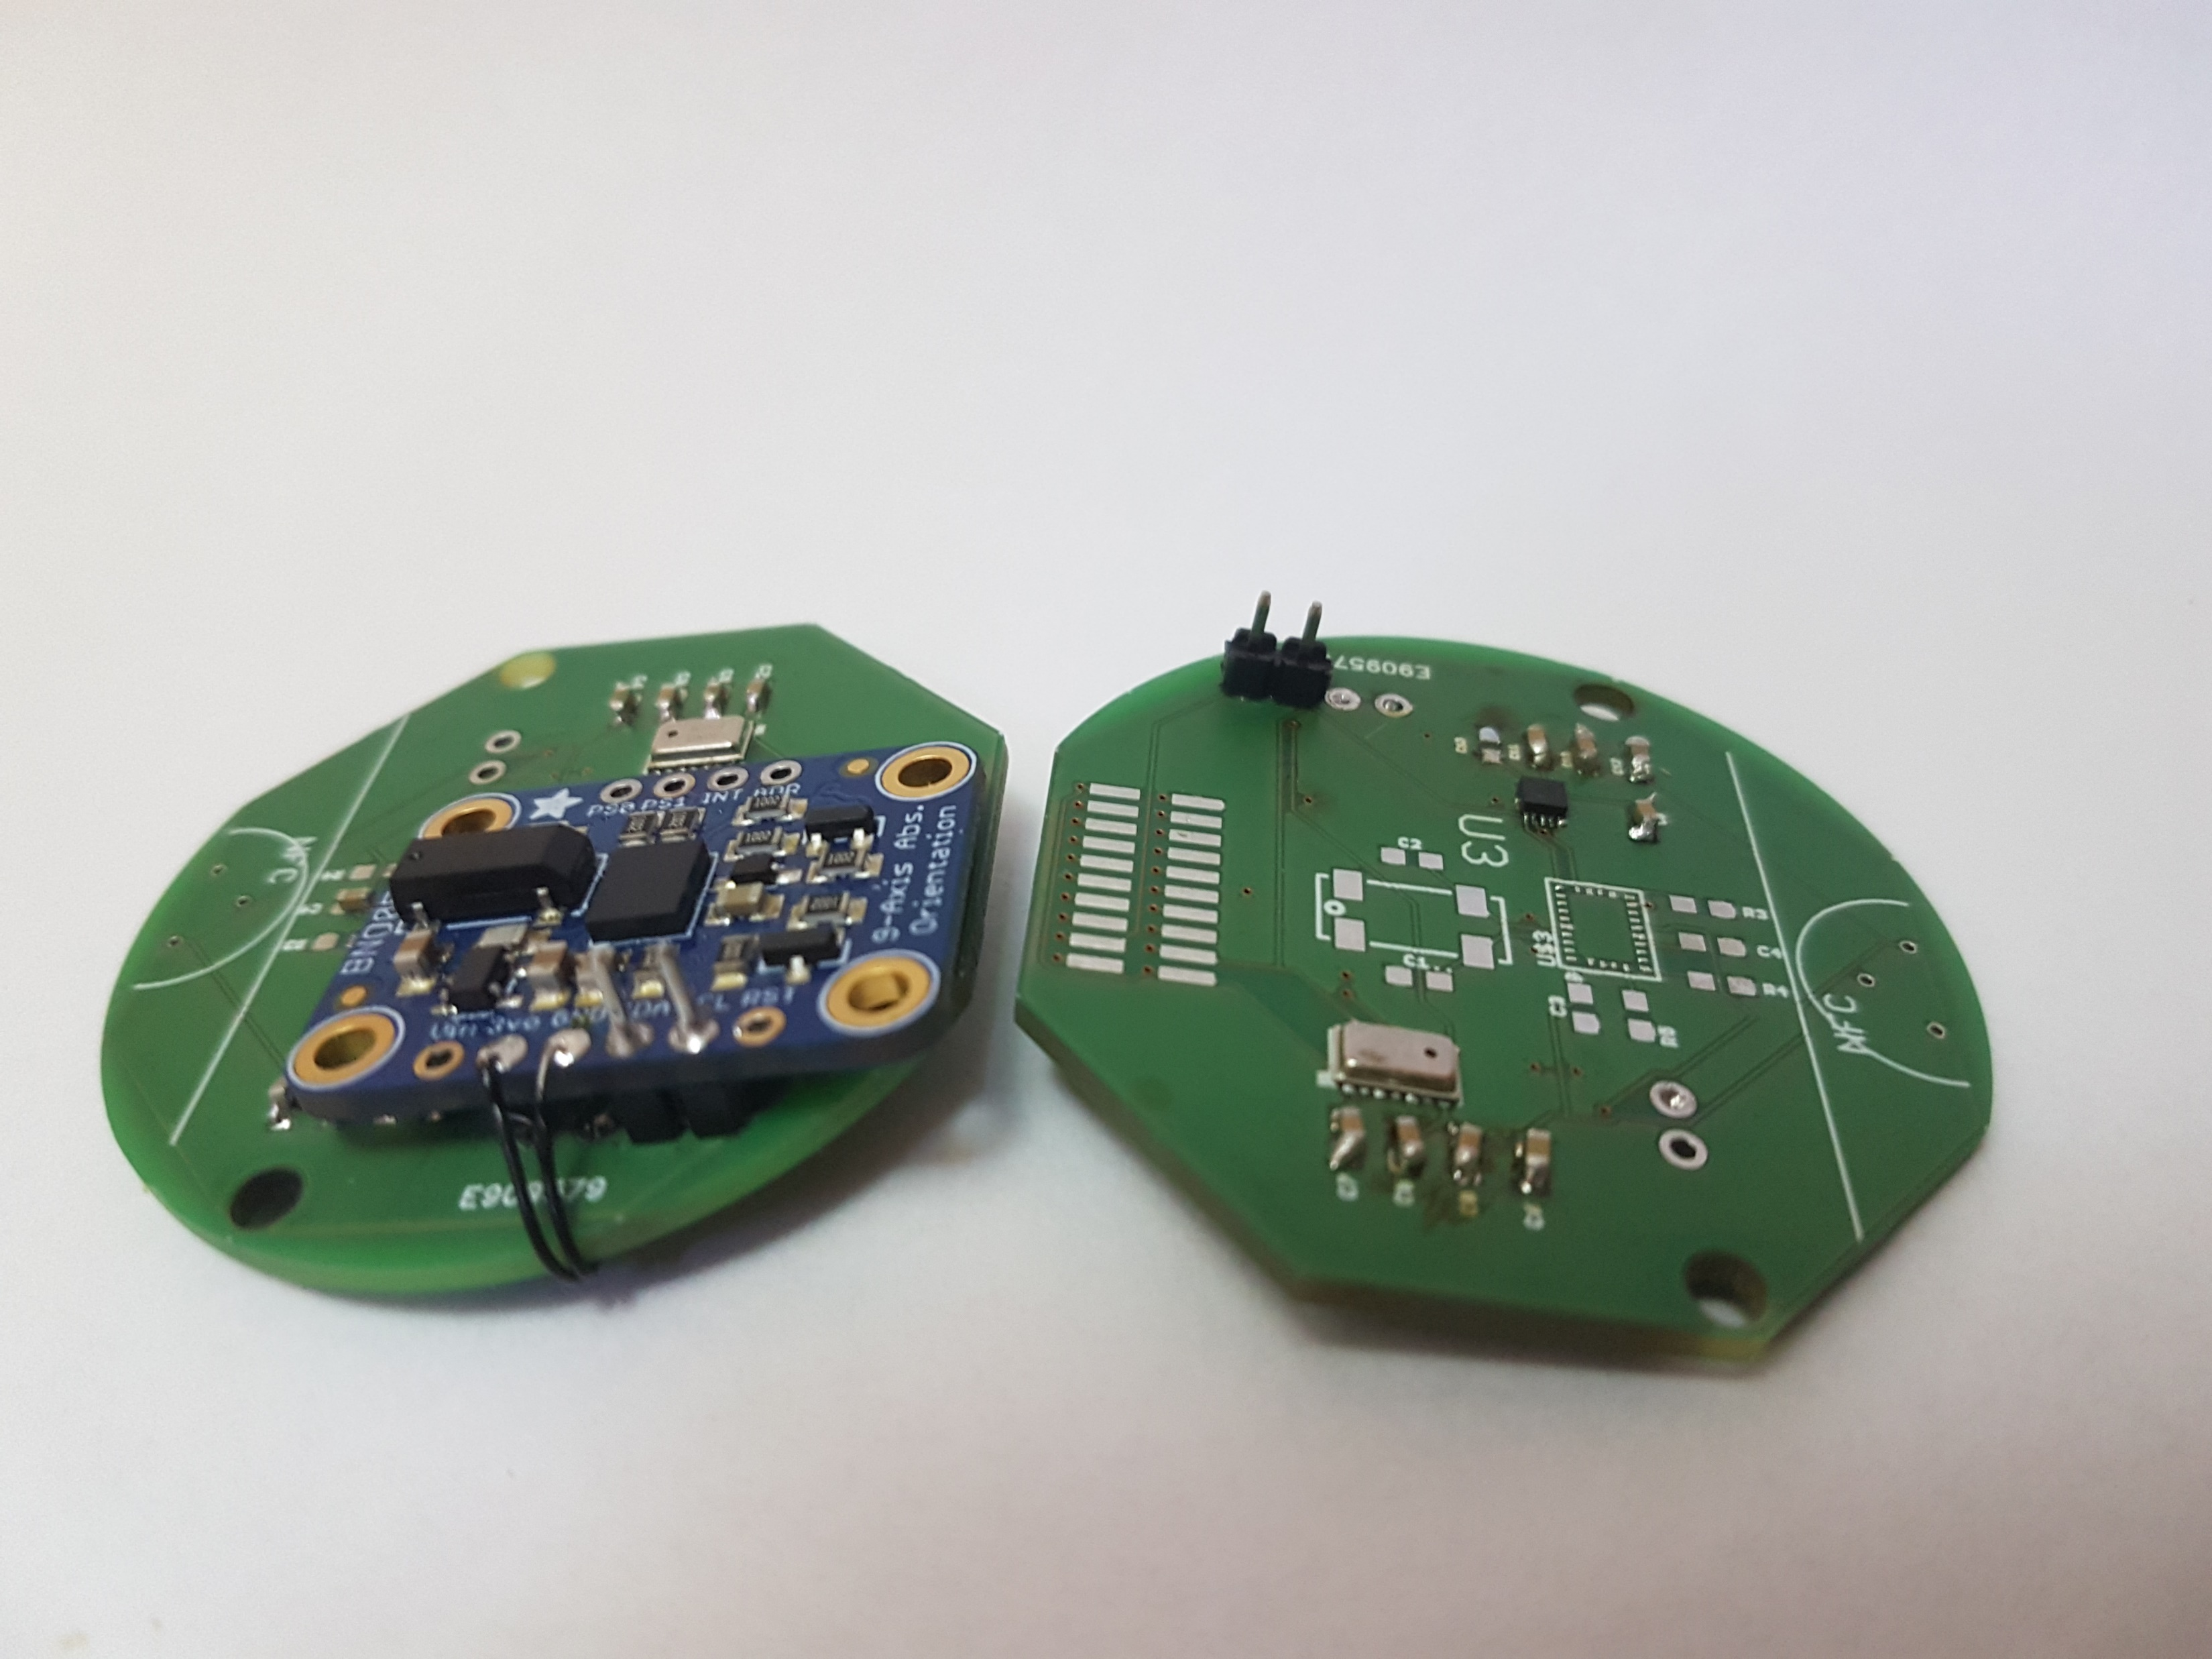
\includegraphics[width=.4\textwidth]{images/mobile2.jpg}}
\end{figure}
\begin{figure}
  \centering
  \subfloat{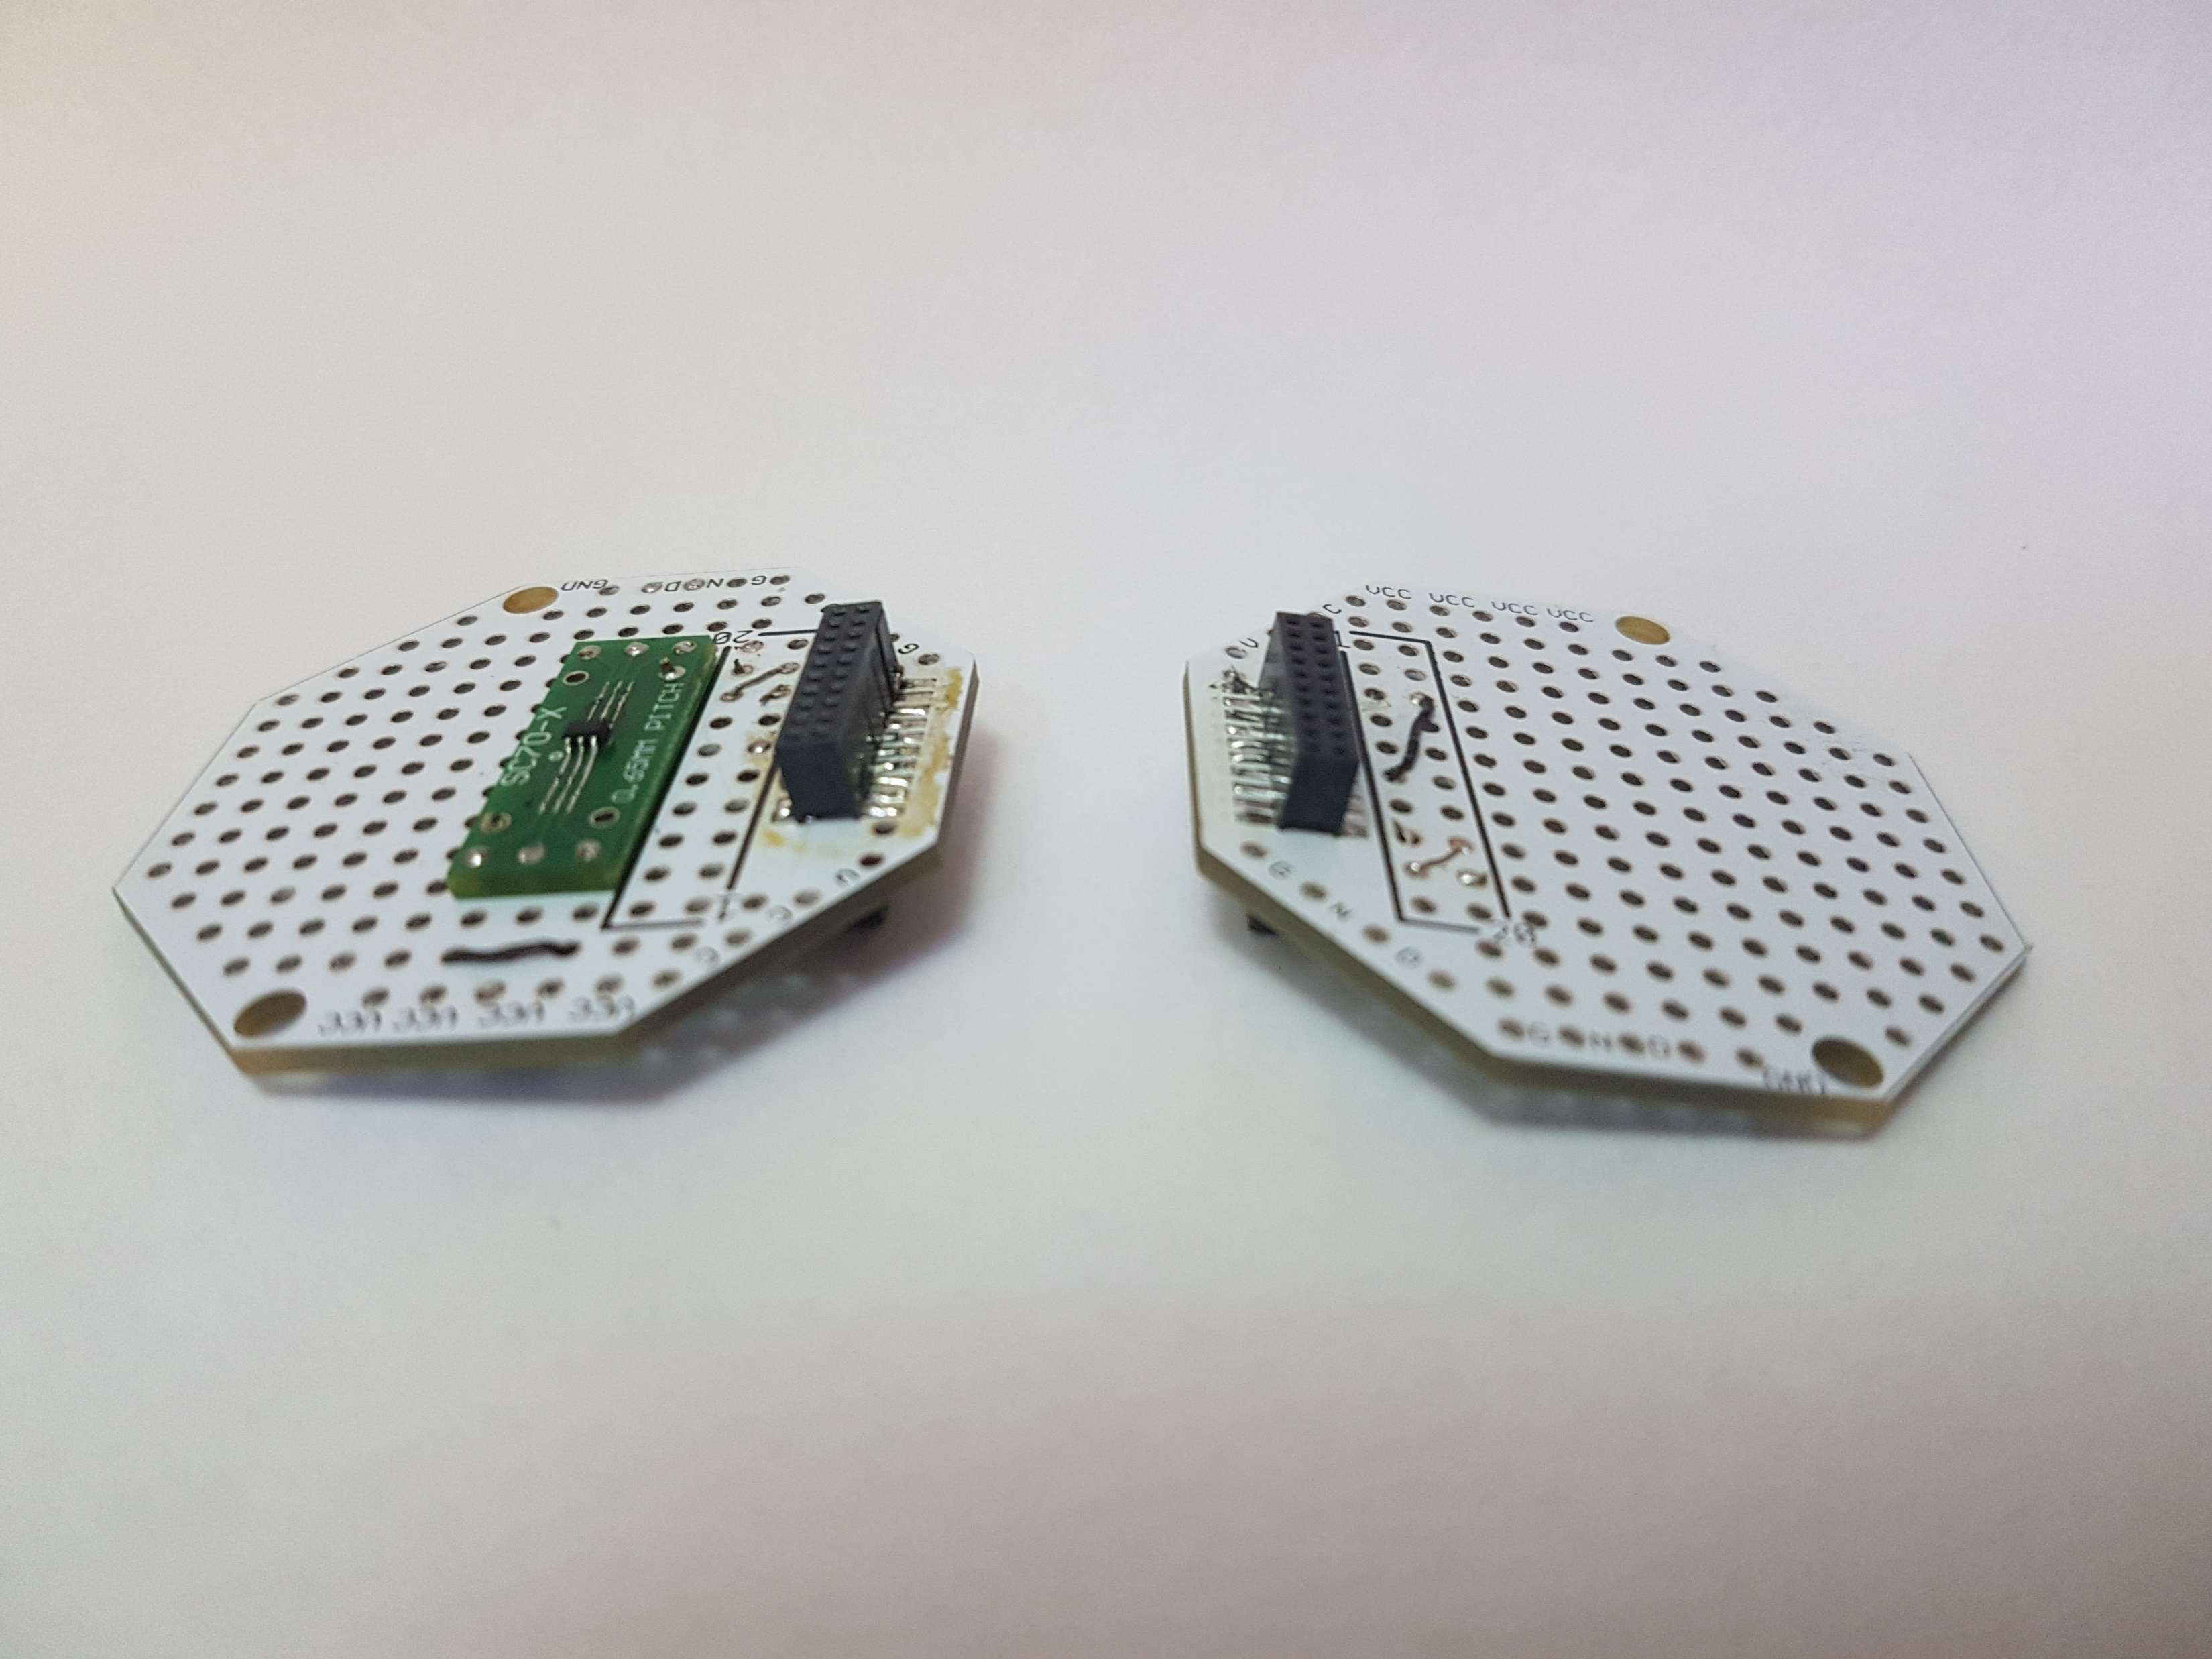
\includegraphics[width=.4\textwidth]{images/mobile3.jpg}}\qquad
  \subfloat{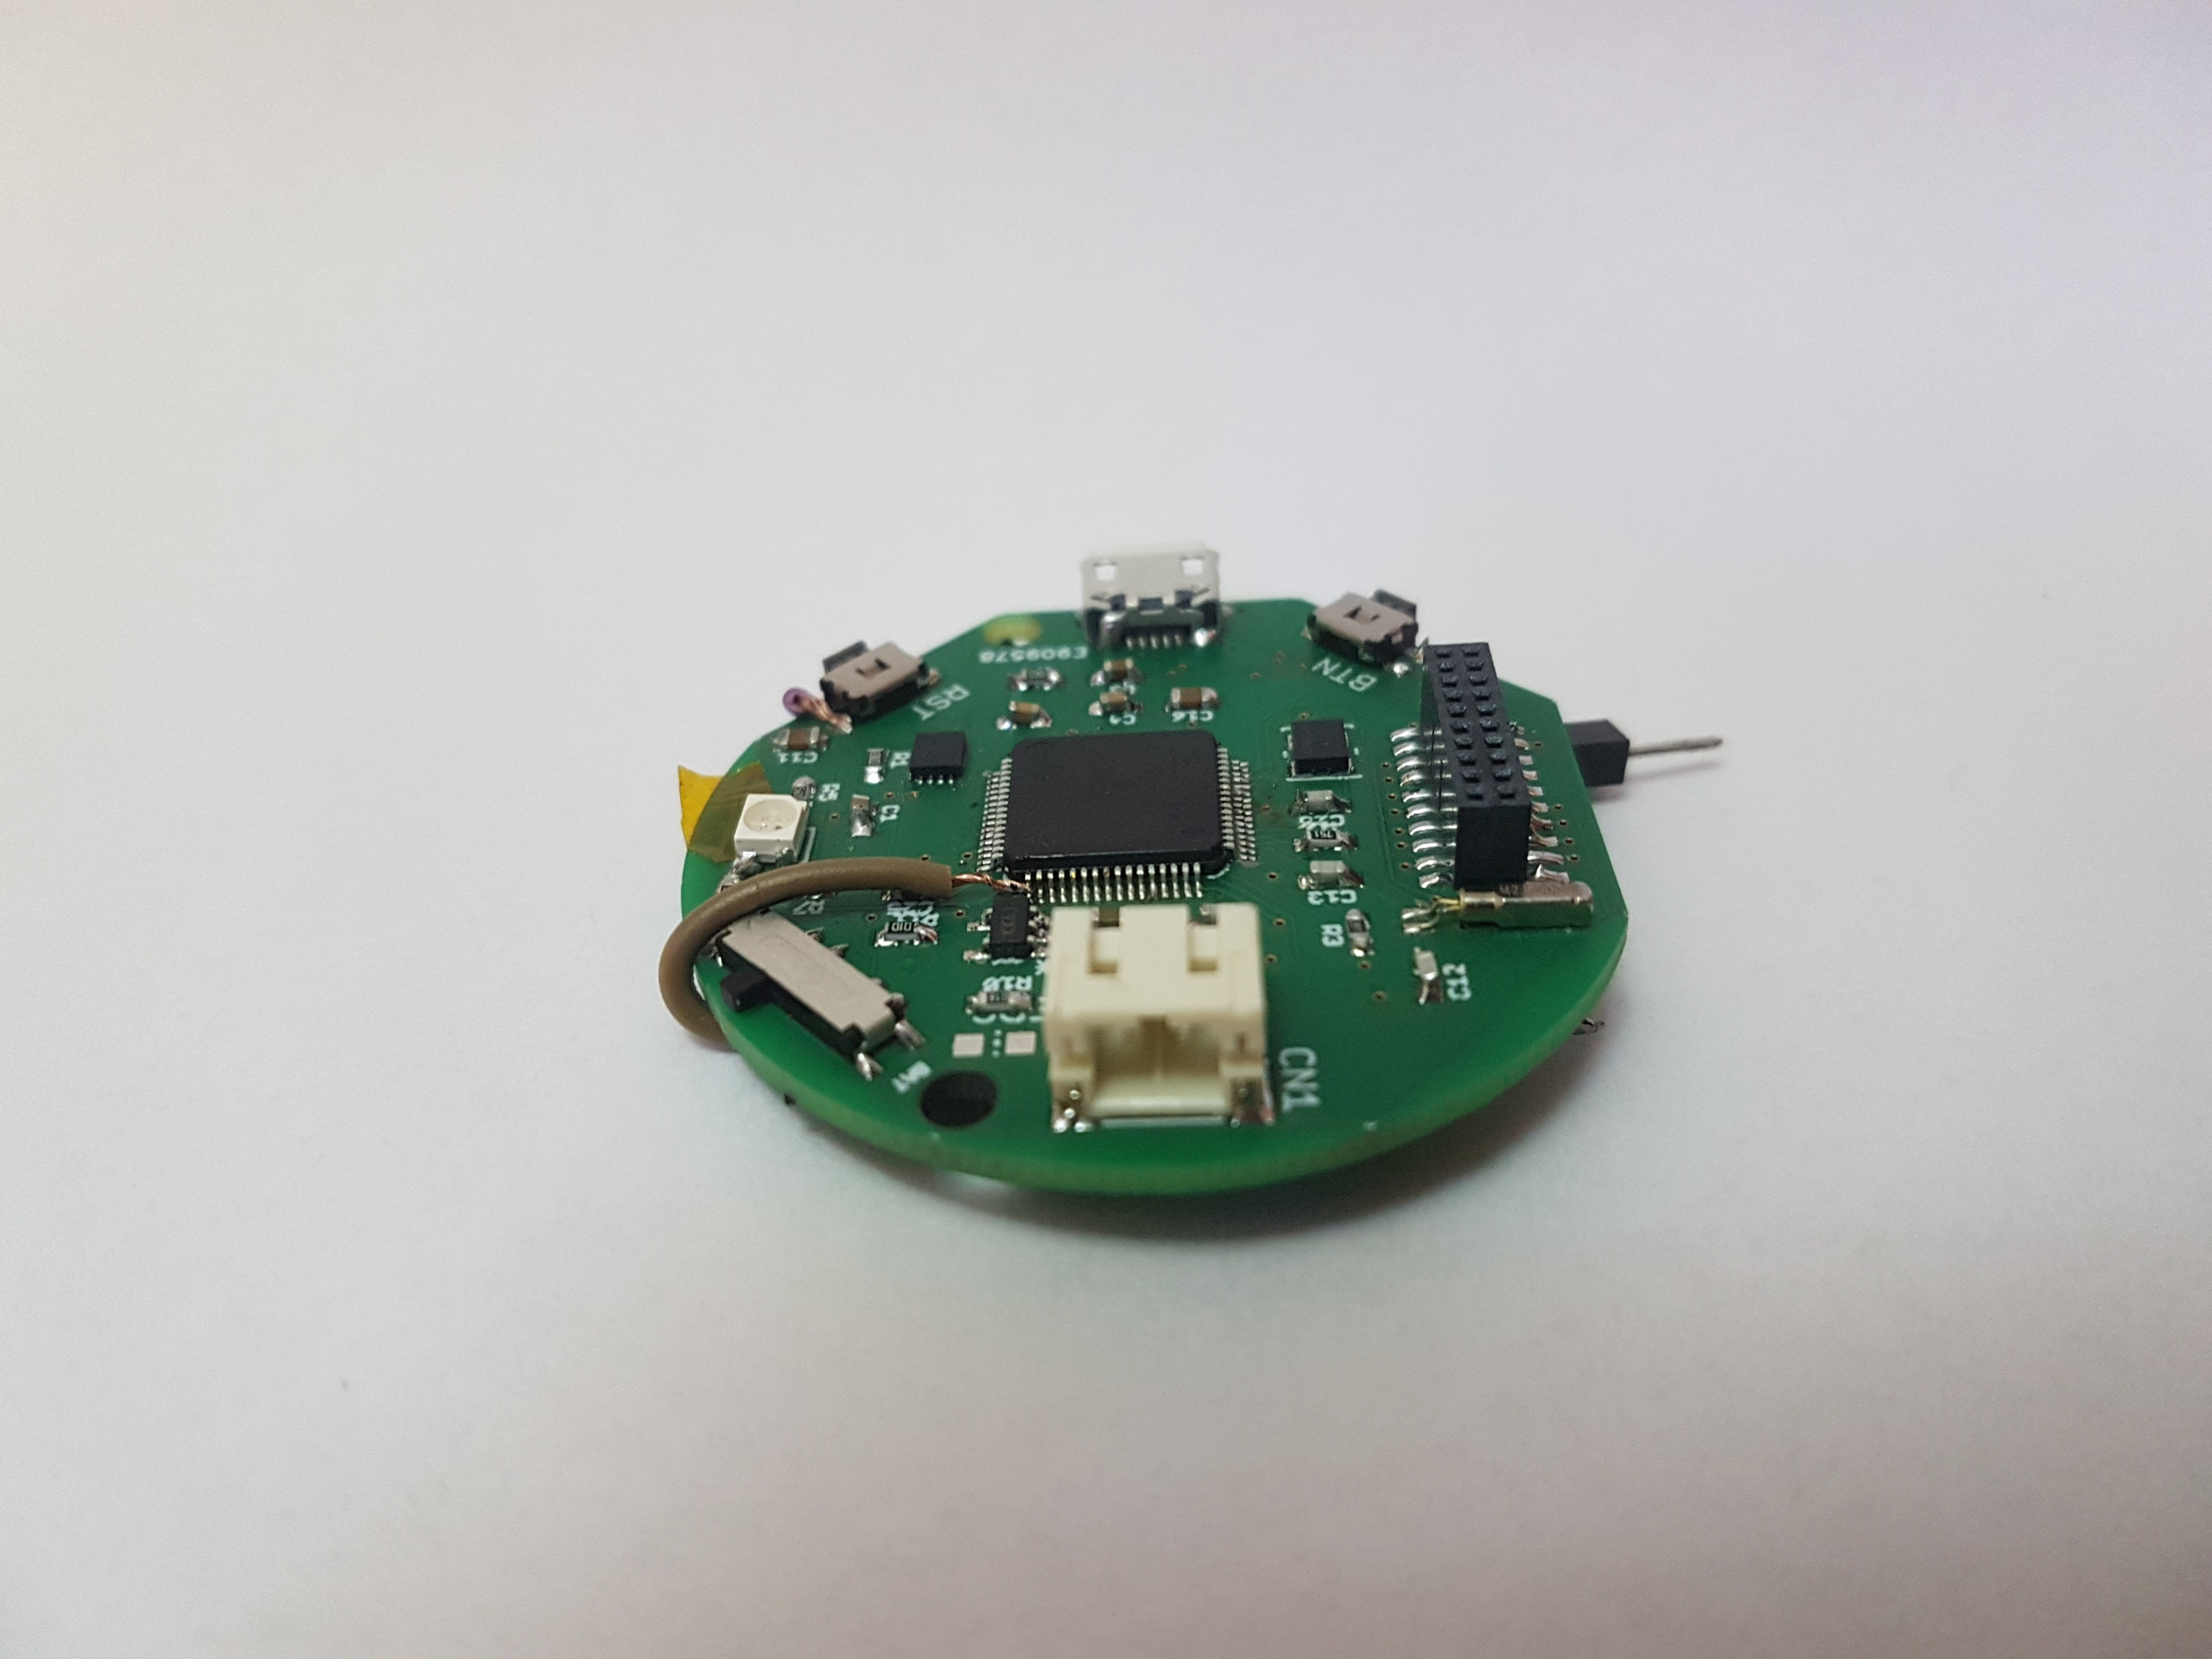
\includegraphics[width=.4\textwidth]{images/mobile4.jpg}}
\end{figure}
\end{frame}

\begin{frame}[fragile]
\frametitle{Mobile Node - Combination} 
\begin{figure}
  \centering
	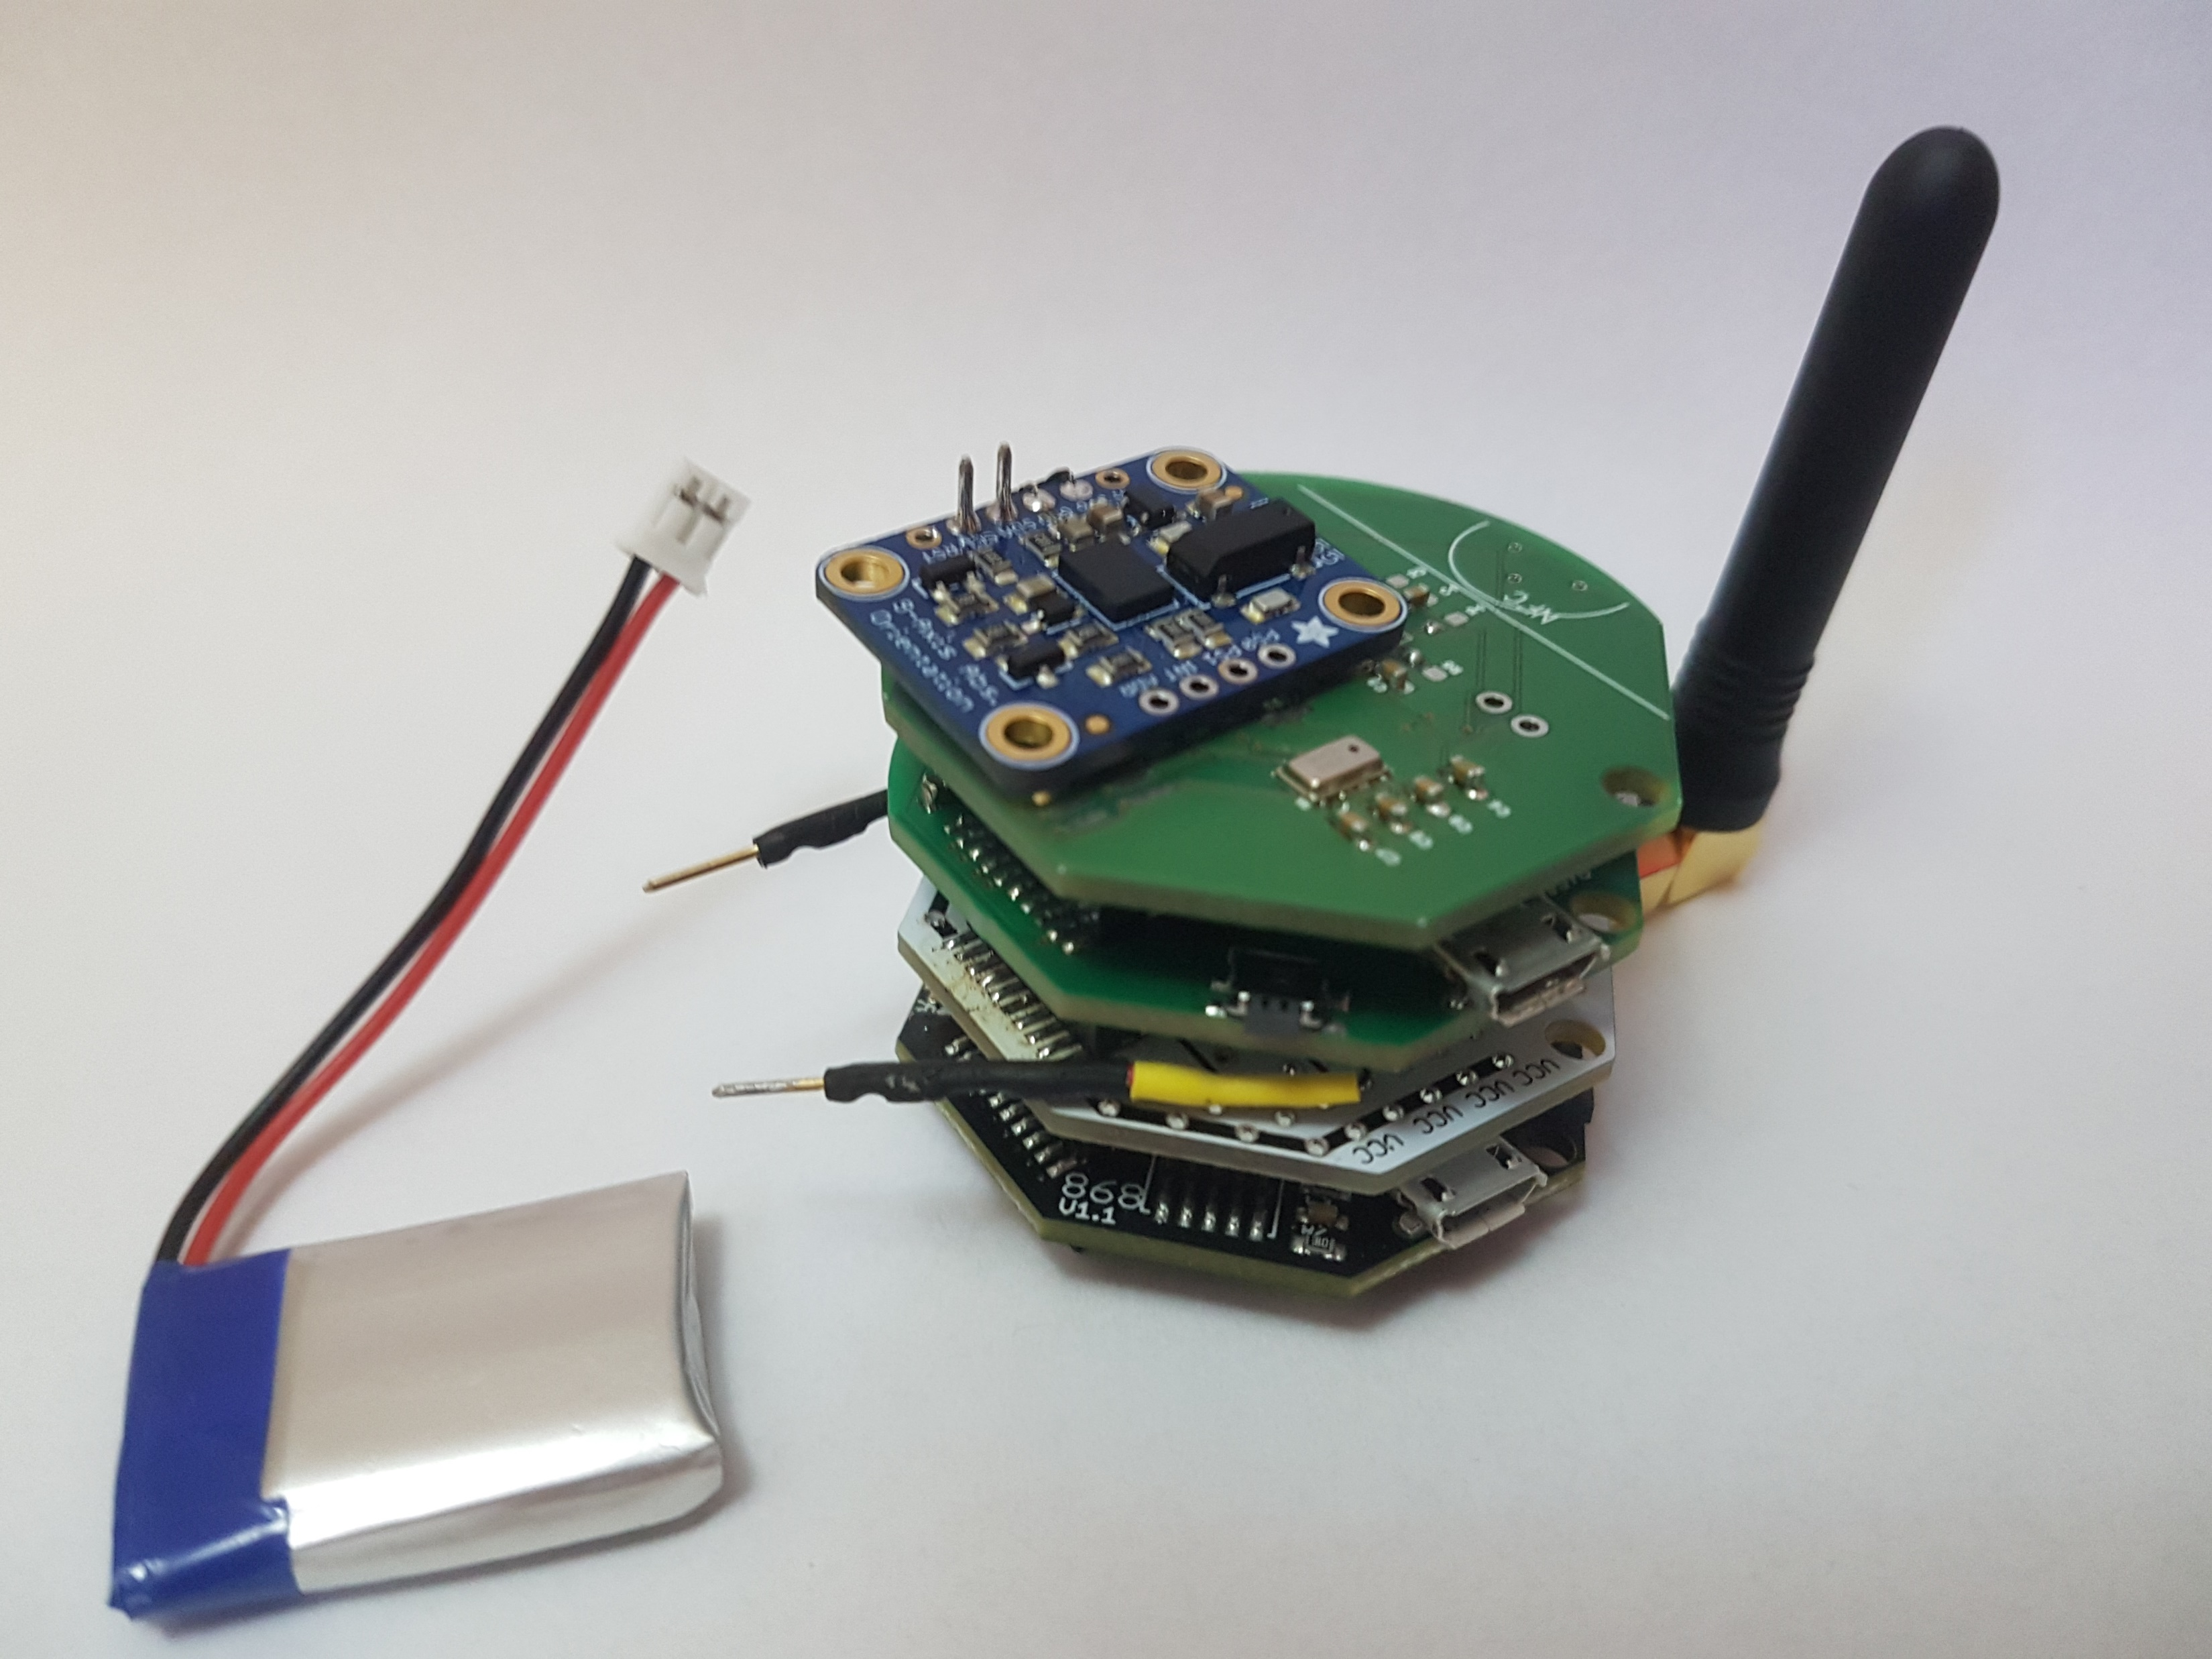
\includegraphics[width=\textwidth]{images/mobile5.jpg}
\end{figure}
\end{frame}

\begin{frame}[fragile]
\frametitle{Mobile Node - Software} 
\begin{figure}
  \centering
	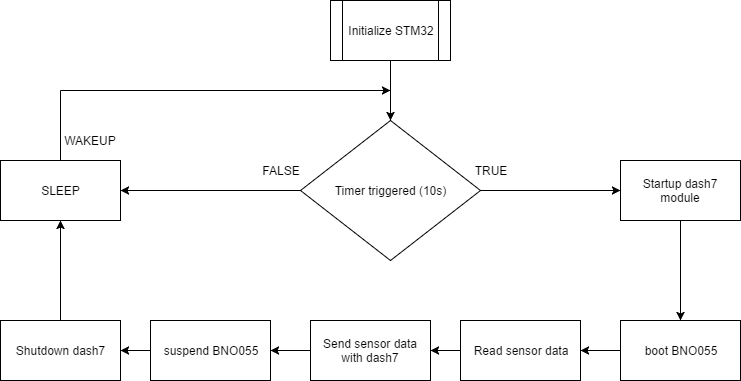
\includegraphics[width=\textwidth]{images/mobile6.png}
\end{figure}
\end{frame}

\begin{frame}[fragile]
\frametitle{Mobile Node - Power Management} 
\begin{figure}
  \centering
  \subfloat{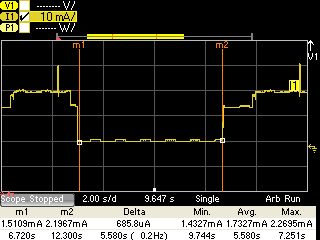
\includegraphics[width=.4\textwidth]{images/Mobile7.jpg}}\qquad
  \subfloat{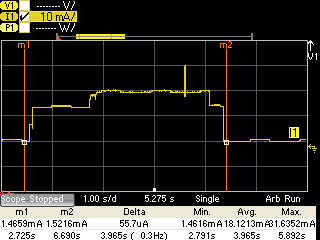
\includegraphics[width=.4\textwidth]{images/Mobile8.jpg}}
\end{figure}
\end{frame}


%%%%%%%%%%%%%%%%%%%%%%%%%%%%%%%%%%%%%%%%%%%%%%%%%%%%%%%%%%%%%%%%%%%%%%%%%%%%%%%%%%%%%%%%%%
\section{Localisation}
%%%%%%%%%%%%%%%%%%%%%%%%%%%%%%%%%%%%%%%%%%%%%%%%%%%%%%%%%%%%%%%%%%%%%%%%%%%%%%%%%%%%%%%%%%

\subsection{Fingerprinting D7}
\begin{frame} 
\frametitle{Localisation}
\begin{itemize}
\item Fingerprinting Dash7
	\begin{center}
  		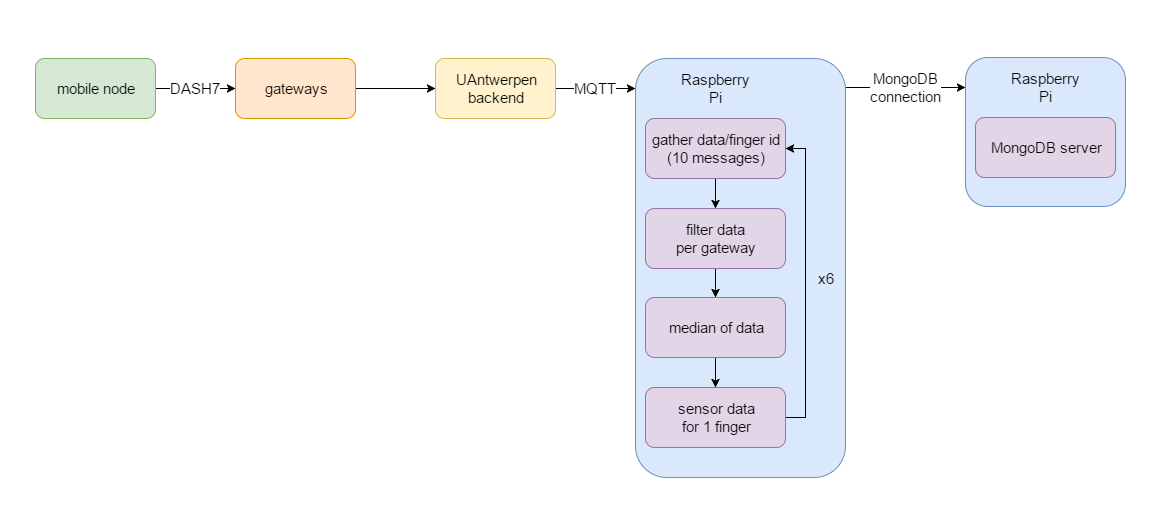
\includegraphics[width=\textwidth]{images/Flowchart.png}
	\end{center}
\end{itemize}
\end{frame}

\note{\begin{itemize}
\item Mobiele node stuurt constant (ongeveer om de 0,5 seconden) berichten die de gateways, verspreid over deze verdieping, ontvangen.
\item Informatie van het transmissiesignaal, zoals de link-budget en het tijdstip worden dan door een server van de UA gepublished via MQTT.
\item Op de RaspberryPi loopt dan een script die deze data van MQTT uitleest. Het script haalt 10 berichten via MQTT binnen per finger id (plaats)
\item Vervolgens wordt deze data gefilterd per gateway. Per elke gateway wordt dan van de ontvangen data de mediaan genomen.
\item Dit wordt per finger id 6 keer herhaald zodat er per locatie 6 querries in de database worden opgeslagen.
\end{itemize}}

\begin{frame} 
\frametitle{Localisation}
\begin{itemize}
\item Fingerprinting Dash7
	\begin{center}
  		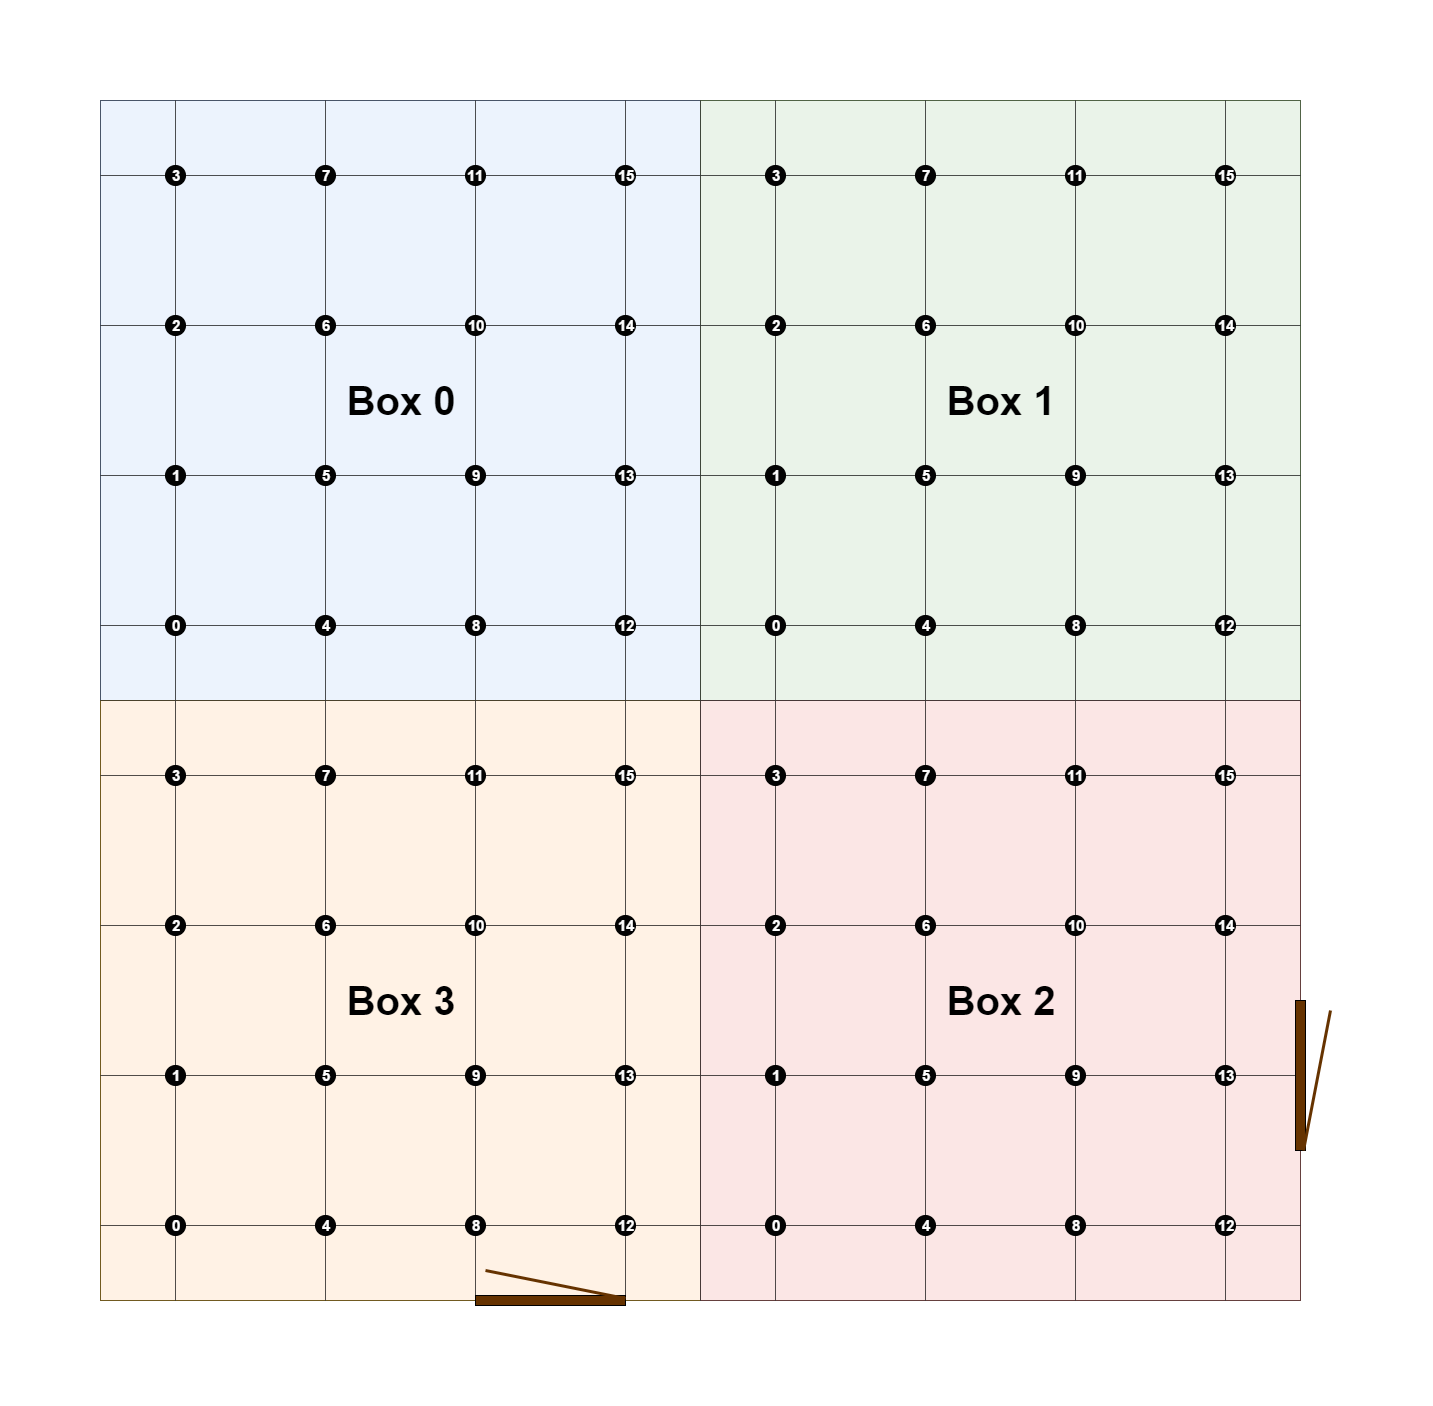
\includegraphics[width=.8\textwidth]{images/V315fingerprint.png}
	\end{center}
\end{itemize}
\end{frame}

\note{\begin{itemize}
\item Dit is een afbeelding om te tonen hoe de data met DASH7 werd gemapt (het gaat hier over V315).
\item De ruimte is in 4 blokken opgedeeld.
\item Elk blok is opgedeeld in 16 fingers, even ver van elkaar verspreid. Voor elke finger werden er 6 querries in de database opgeslagen zoals eerder vermeld.
\end{itemize}}

\subsection{Dash7}
\begin{frame} 
\frametitle{Localisation}
\begin{itemize}
\item Dash7
	\begin{center}
  		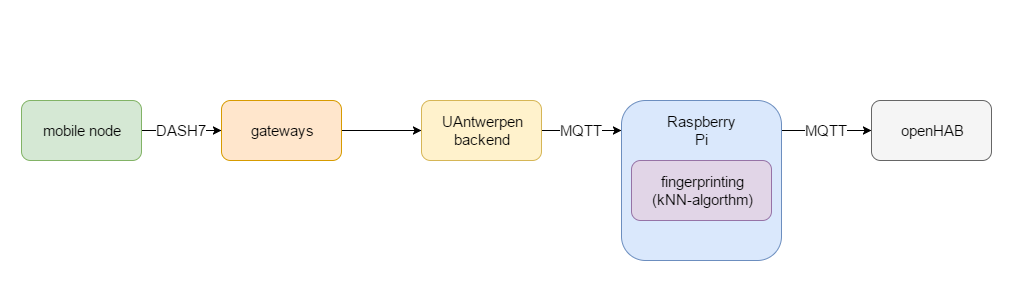
\includegraphics[width=\textwidth]{images/Flowchart3.png}
	\end{center}
\end{itemize}
\end{frame}

\note{\begin{itemize}
\item De mobiele node stuurt constant DASH7 berichten.
\item De gateways sturen transmissie gegevens door naar een server van de UA die deze data published via MQTT.
\item De RaspberryPi leest deze data uit en past hierop het kNN-algoritme toe voor fingerprinting.
\item De uitkomst (locatie) wordt dan door de RaspberryPi gepublished via MQTT zodat dit kan uitgelezen worden op openHAB
\end{itemize}}

\begin{frame} 
\frametitle{Localisation}
\begin{itemize}
\item Dash7
	\begin{center}
  		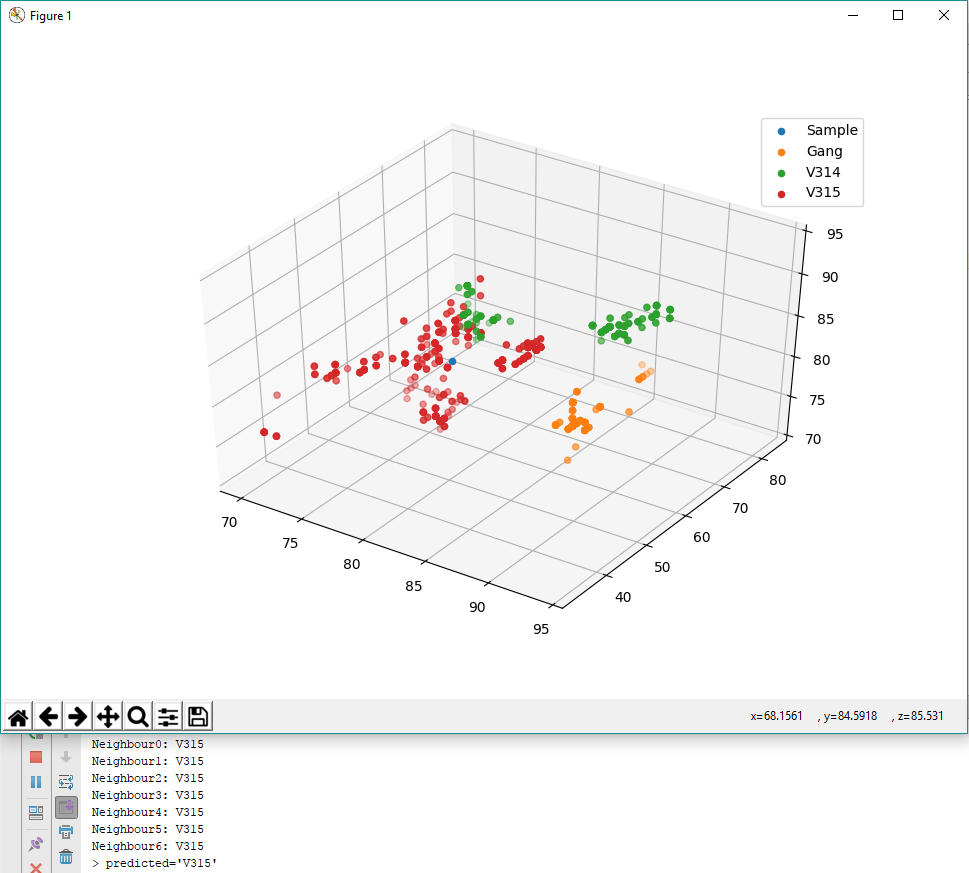
\includegraphics[width=.7\textwidth]{images/GraphicDASH7.PNG}
	\end{center}
\end{itemize}
\end{frame}

\note{\begin{itemize}
\item Dit is een grafiek die de data-link waardes weergeeft op een grafiek.
\item Deze afbeelding zou normaal 6-dimentionaal moeten zijn omdat er 6 gateways zijn maar omdat dit niet visueel mogelijk was hebben we gekozen om het 3-dimentionaal weer te geven met de 3 belangrijkste gateways.
\end{itemize}}

\subsection{Fingerprinting MAG}
\begin{frame} 
\frametitle{Localisatie}
\begin{itemize}
\item Fingerprinting Magnetometer
	\begin{center}
  		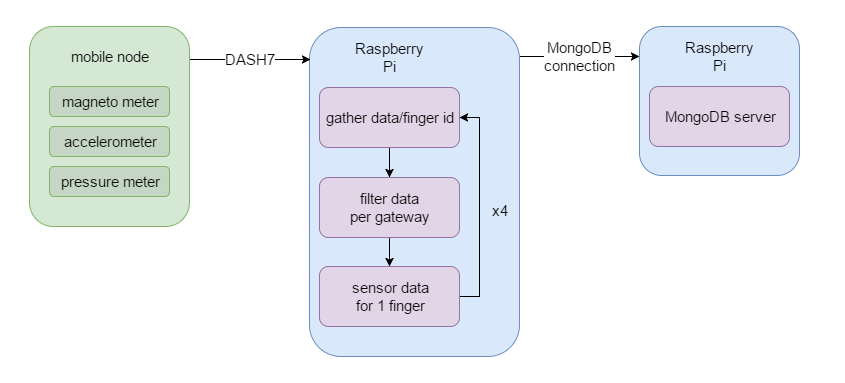
\includegraphics[width=\textwidth]{images/Flowchart2.png}
	\end{center}
\end{itemize}
\end{frame}

\note{\begin{itemize}
\item Mobiele node stuurt constant berichten via DASH7 met data in van de magneto meter, accelerometer en barometer.
\item Op de RaspberryPi loopt een script die deze data via DASH7 ontvangt.
\item Per finger id (plaats) worden er 4 querries in de database gezet.
\end{itemize}}

\subsection{Magnetometer}
\begin{frame} 
\frametitle{Localisatie}
\begin{itemize}
\item Magnetometer
	\begin{center}
  		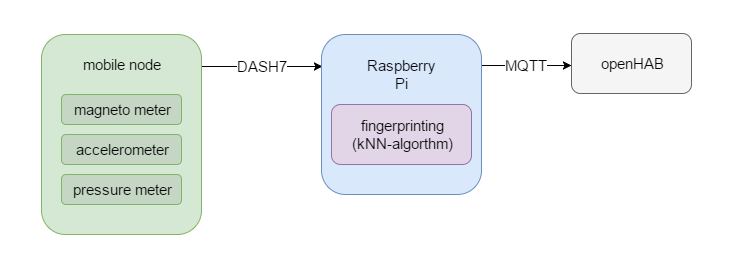
\includegraphics[width=\textwidth]{images/Flowchart4.png}
	\end{center}
\end{itemize}
\end{frame}

\note{\begin{itemize}
\item Mobiele node stuurt constant berichten via DASH7 met data in van de magneto meter, accelerometer en barometer.
\item Op de RaspberryPi loopt een script die deze data via DASH7 ontvangt.
\item Op deze data wordt het kNN-algoritme toegepast voor fingerprinting.
\item De uitkomst (locatie) wordt dan door de RaspberryPi gepublished via MQTT zodat dit kan uitgelezen worden op openHAB.
\end{itemize}}

\subsection{kNN-Algorithm}
\begin{frame} 
\frametitle{kNN-Algorithm}
\begin{itemize}
\item Dash7
	\begin{itemize}
	\item k = 7
	\end{itemize}
\item Magnetometer
	\begin{itemize}
	\item k = 5
	\end{itemize}
\item Distance metric
	\begin{itemize}
	\item Euclidean distance
	\item Manhattan distance
	\end{itemize}
\end{itemize}
\end{frame}

\note{\begin{itemize}
\item Voor DASH7 lokalisatie wordt k=7 gebruikt
\item Voor Magnetometer lokalisatie wordt k=5 gebruikt
\item Als distance metric wordt Manhattan distance gebruikt omdat deze nauwkeuriger is dan Euclidean distance voor meerdere gateways.
\end{itemize}}

%%%%%%%%%%%%%%%%%%%%%%%%%%%%%%%%%%%%%%%%%%%%%%%%%%%%%%%%%%%%%%%%%%%%%%%%%%%%%%%%%%%%%%%%%%
\section{Gateway}
%%%%%%%%%%%%%%%%%%%%%%%%%%%%%%%%%%%%%%%%%%%%%%%%%%%%%%%%%%%%%%%%%%%%%%%%%%%%%%%%%%%%%%%%%%

\subsection{Sensors}

\begin{frame} 
\frametitle{Gateway}
  \begin{itemize}
  \item Sensors \\
  	\begin{center}
  		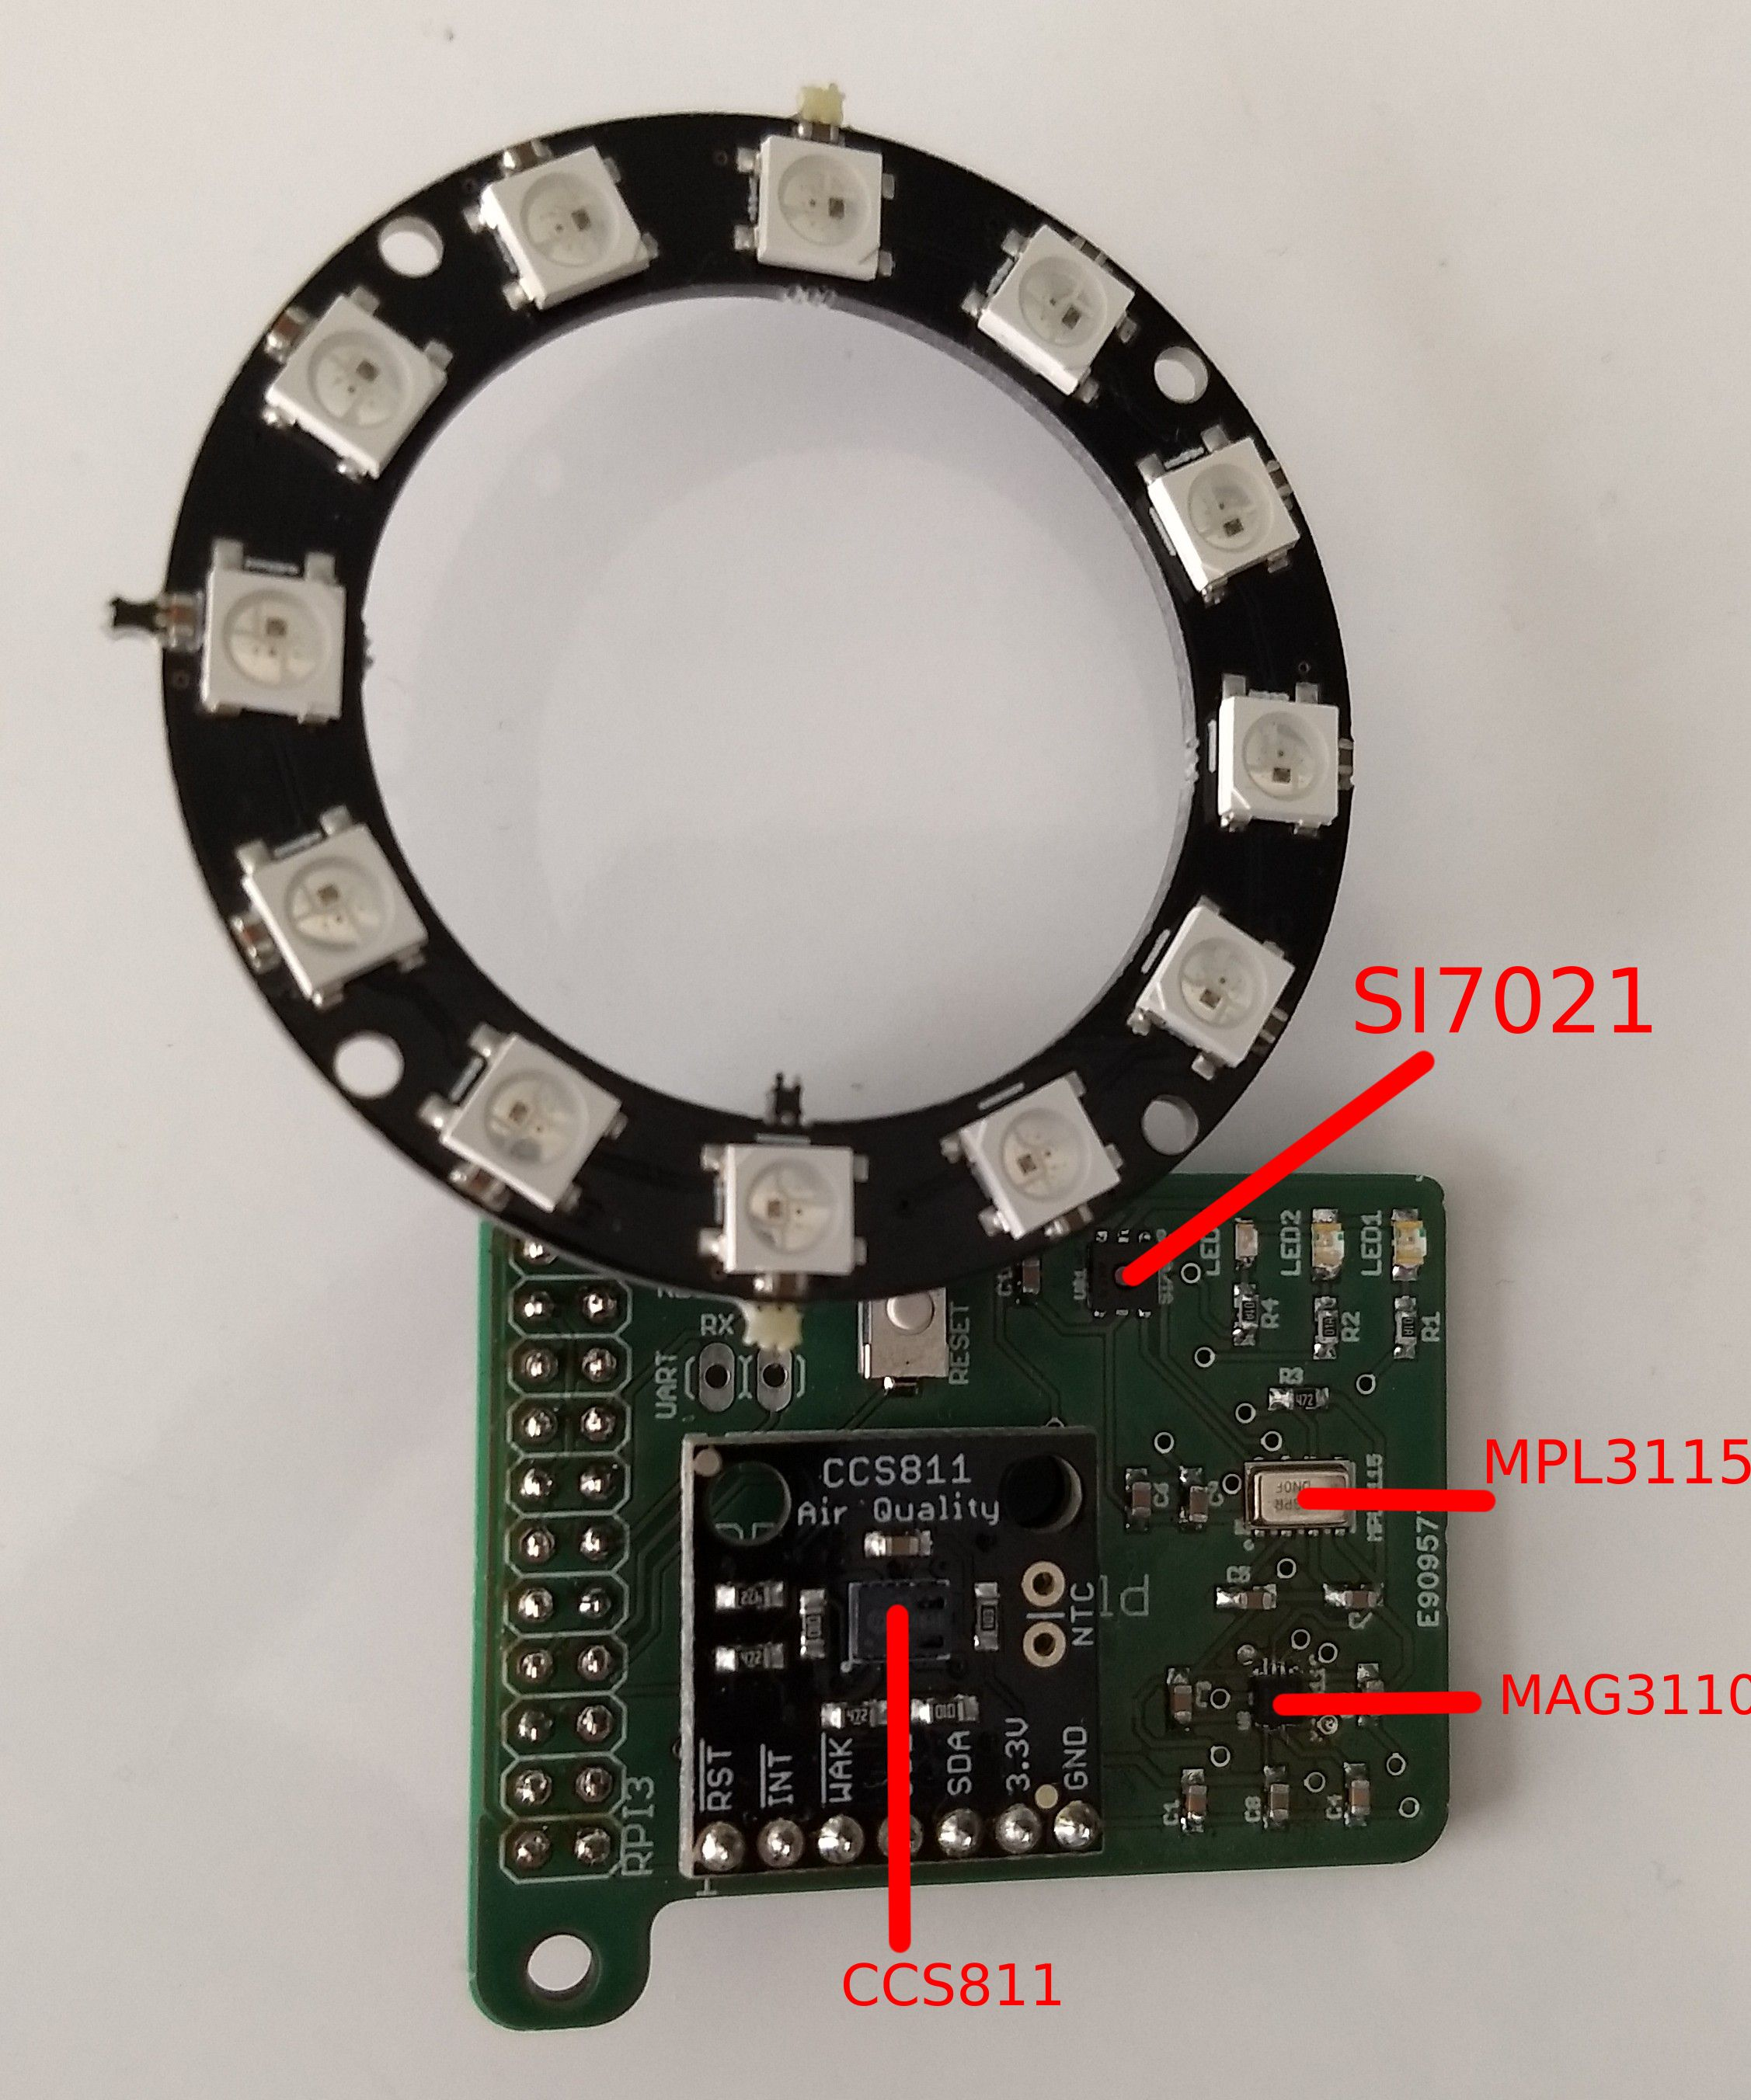
\includegraphics[width=.4\textwidth]{images/RPISensors.jpg}
	\end{center}
  \pause
  \note{\begin{itemize}
		\item CO2 (CCS811): Maakt gebruik van de BCM2835-library, ook gebruikt voor de eerste taken rond de STM-bordjes
		\item Andere sensoren maken gebruik van de standaard I2C-library in Linux.
			\begin{enumerate}
				\item MPL3115, adres is 0x60: Bit 1-3 geven druk en 4-5 temperatuur
				\item SI7021, adres is 0x40: 
					\begin{itemize}
						\item commando 0xF3, leest temperatuur uit
						\item commando 0xF5, leest vochtigheid uit
					\end{itemize}
				\item MAG3310, magnetometer ook op sensorbord maar niet ge\"{i}mplementeerd in project.
			\end{enumerate}
		\end{itemize}}
	\item Sensorvalues published on MQTT topics
  \end{itemize}
\end{frame}

\note{\begin{itemize}
\item We hebben functies geschreven om alle data apart te lezen van de sensoren. Deze 		functies worden aangeroepen door een MAIN-functie. De gelezen waarden worden gefilterd (foute lezingen) en op verschillende MQTT Topics gezet 
	\begin{enumerate}
	\item rpi/temperature, rpi/humidity, rpi/pressure, rpi/airquality
	\end{enumerate}
\end{itemize}}

\subsection{LED Visualisatie}

\begin{frame} 
\frametitle{Gateway}
  \begin{itemize}
  \item LED Visualisation: \\
  \begin{enumerate}
  	\item Profiles
  	\item CO\textsubscript{2} en Temperature Levels
  \end{enumerate}
  	\begin{center}
  		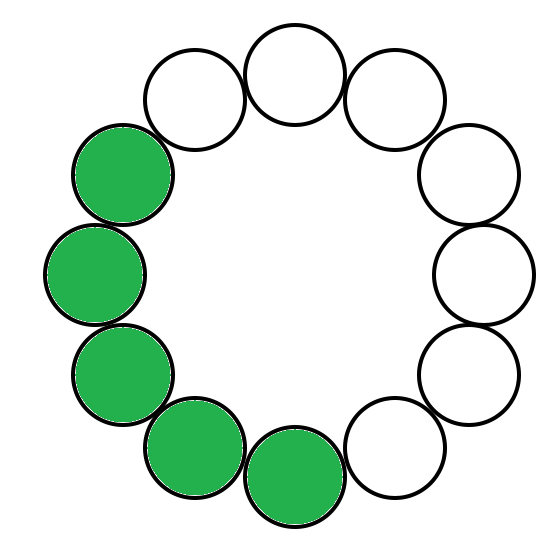
\includegraphics[width=.5\textwidth]{images/LEDlow.png}
  		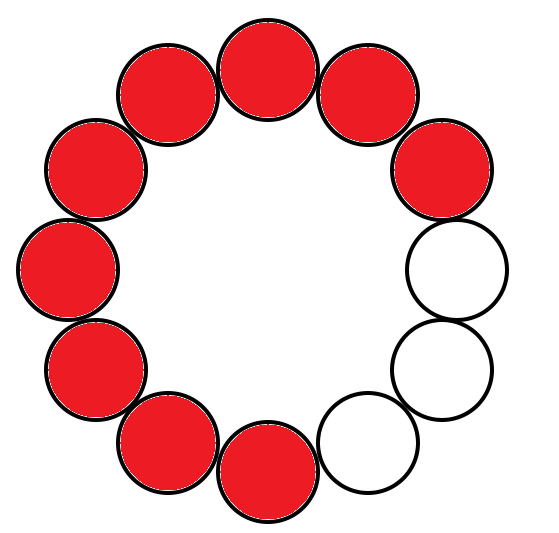
\includegraphics[width=.5\textwidth]{images/LEDhigh.png}
	\end{center}
  \end{itemize}
\end{frame}

\note{\begin{itemize}
\item LEDs worden aangestuurd via een python script. Dit script wordt aangeroepen via het algemeen sensorscript, geschreven in C. 
\item Een script leest temperatuur/CO2 waarden uit, steekt ze in een variabele van Python en runt het script. De kleur geeft de luchtkwaliteit weer (Groen = goed, rood = slecht), het aantal ledjes geeft de temperatuur weer.
\item CO\textsubscript{2}: 400-1400ppm en Temperatuur: 19-35 graden
\item Als er iemand binnenkomt, nemen de leds een preference color aan a.d.h.v. de id van RFID chip. De kleur word geoverride bij de volgende temperatuur/CO2-meting.
\end{itemize}}

\subsection{Extra's}
\begin{frame} 
\frametitle{Gateway}
  \begin{itemize}
  \item Camera \\
  \begin{center}
  		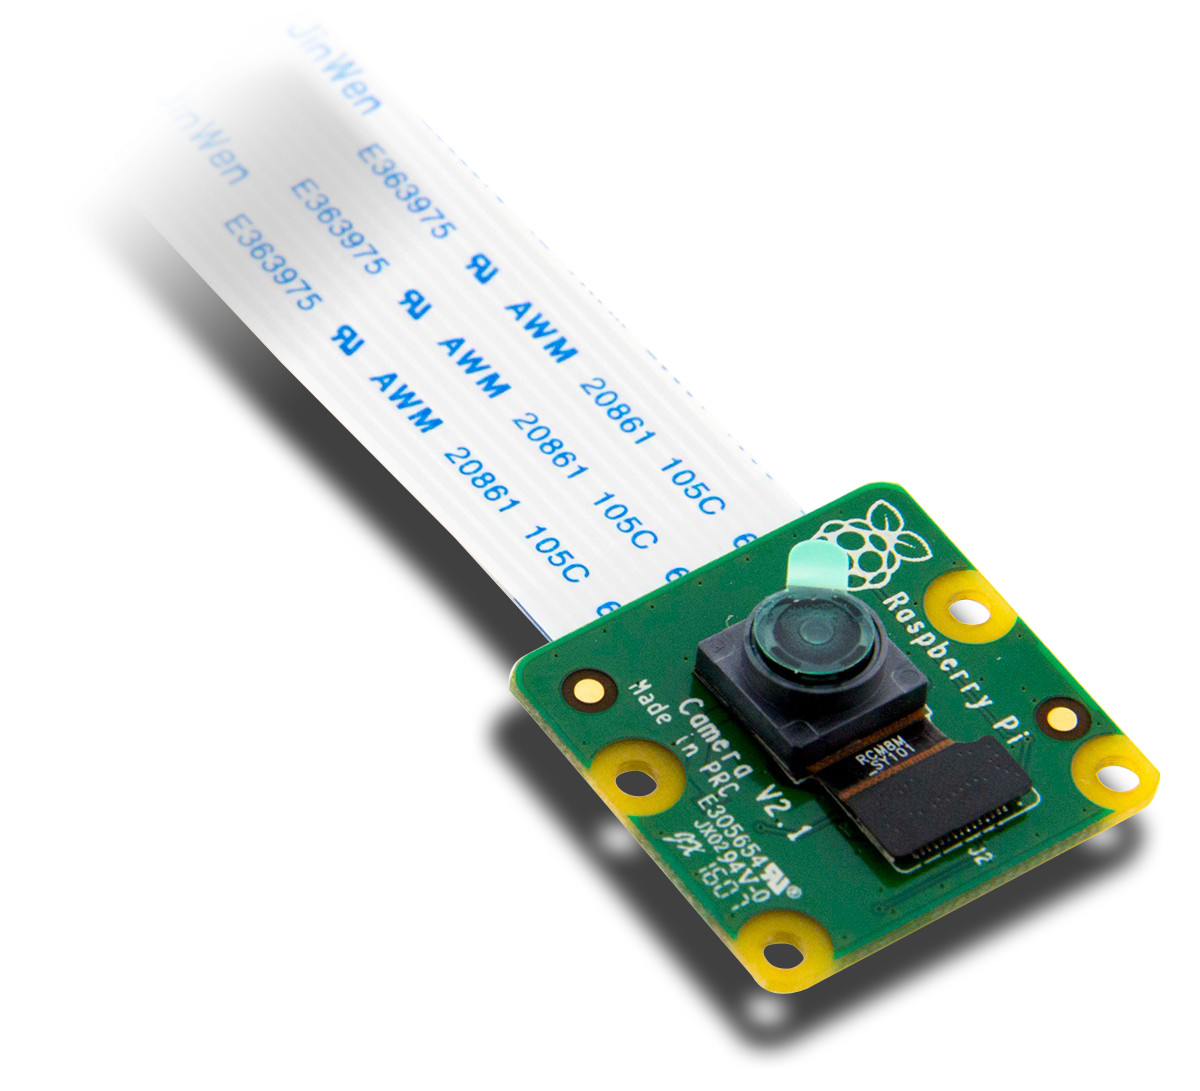
\includegraphics[width=.4\textwidth]{images/piCam.jpg}
	\end{center}
  \item Scripts
  \end{itemize}
\end{frame}

\note{\begin{itemize}
\item Camera script neemt foto en plaats dit in openhab folder
\item Extra script om RFID inlog/presence te loggen, aangeroepen bij aankomst van dash7 bericht
\item Crontab
	\begin{enumerate}
	\item start camera bij startup
	\item start sensorlezing RPI bij startup
	\item elke 30sec sensorlezing
	\item gegevens van crontab worden ook weggeschreven in log
	\item Dash7 localisatie starten
	\item Dash7 module om gegevens van mobile node te krijgen
	\end{enumerate}
\end{itemize}}

%%%%%%%%%%%%%%%%%%%%%%%%%%%%%%%%%%%%%%%%%%%%%%%%%%%%%%%%%%%%%%%%%%%%%%%%%%%%%%%%%%%%%%%%%%
\section{openHAB}
%%%%%%%%%%%%%%%%%%%%%%%%%%%%%%%%%%%%%%%%%%%%%%%%%%%%%%%%%%%%%%%%%%%%%%%%%%%%%%%%%%%%%%%%%%

\begin{frame} 
\frametitle{openHAB}
  \begin{itemize}
  \item Basic UI \\
  \begin{center}
  		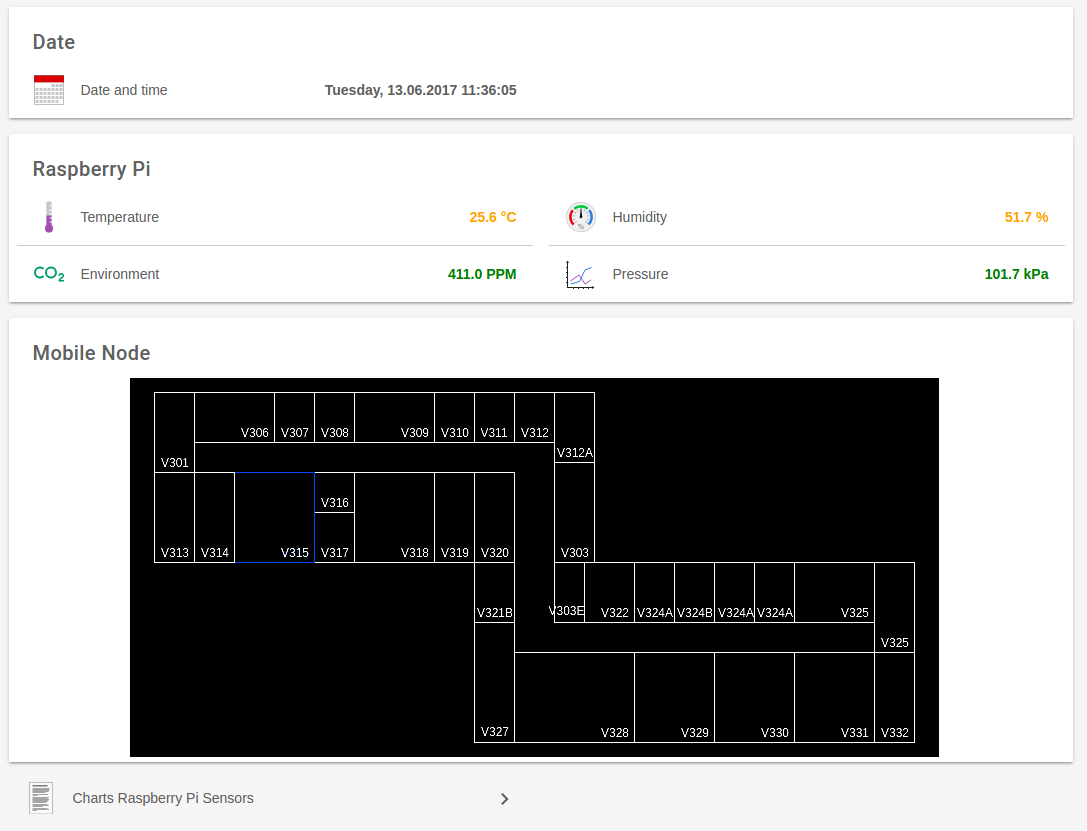
\includegraphics[width=.8\textwidth]{images/basicUI.png}
	\end{center}
	\item HabPanel
  \end{itemize}
\end{frame}

\note{\begin{itemize}
\item Gestart met Basic UI omdat het makkelijker is om items uit te lezen.
\item Overgeschakeld naar HabPanel voor presentatie
\item Custom widgets aangemaakt in html gebruik makend van bootstrap
\item Cusom widgets voor RPI, Mobile node sensoren
\item Custom widget voor Live Weer updates
\item Basic widgets voor afbeeldingen en tekstbestanden
\end{itemize}}

%%%%%%%%%%%%%%%%%%%%%%%%%%%%%%%%%%%%%%%%%%%%%%%%%%%%%%%%%%%%%%%%%%%%%%%%%%%%%%%%%%%%%%%%%%
\section{Future Work}
%%%%%%%%%%%%%%%%%%%%%%%%%%%%%%%%%%%%%%%%%%%%%%%%%%%%%%%%%%%%%%%%%%%%%%%%%%%%%%%%%%%%%%%%%%

\begin{frame} 
\frametitle{Future Work}
  \begin{itemize}
  \item Alexa is installed, this can be combined with OpenHAB
  \item Magnetometer localisation
  \item Combine localisation node with mobile node
  \end{itemize}
\end{frame}

%%%%%%%%%%%%%%%%%%%%%%%%%%%%%%%%%%%%%%%%%%%%%%%%%%%%%%%%%%%%%%%%%%%%%%%%%%%%%%%%%%%%%%%%%%
\end{document}
%%%%%%%%%%%%%%%%%%%%%%%%%%%%%%%%%%%%%%%%%%%%%%%%%%%%%%%%%%%%%%%%%%%%%%%%%%%%%%%%%%%%%%%%%%